
%% %%
%% %% INTRO
%% %%

\slide{ A vs C side asymmetry: W vs Z }
{

 \iteb
 \item 2011 data, MC11c, combined STACO muons
 \item Inclusive W analysis: $p_T^{\mu}>25$, $E_T^{Miss}>25$, $m_T^{W}>40$, $p_{T}^{iso R=40}/p_{T}<0.1$
 \item Missing ET: MetREFFinal
 \item Single-muon trigger (18 GeV) used both for Ws and Zs
 \iteb
 \item In plots below, both Z muons are required to have fired the trigger
 \itee
 \item Reconstruction, trigger, isolation scale factors are computed in $\eta$ bins of measurement.
 \item Disagreements in A-side to C-side ratio
 \item Focus on last 4 \eta\ bins
 \itee

}

\slide{ A-C ratios }
{

\only<1>{
 A/C ratios for data, background-subtracted data, and signal MC. \\

 Let's start with the nominal W selection
}

\only<3>{ Next, consider muons in Z selection. First, without explicit trigger match. }
\only<5>{ Adding trigger match requirement to both Z muons. }
\only<7>{ Is it MET? Let's try to re-build it in Ws from LocHadTopo using actual muon }
\only<10>{ It turns out curvature correction ``C'' has noticeable effect on A/C. \\
It might be beneficial to update it using the 2012 MCP machinery. \\
Still, there are still substantial disagreements remaining. Let's drop MET completely.
}

\only<12>{
  Conclusions:\\
  \iteb
    \item Z with trigger match reproduces overall A/C shape seen in W
    \item A/C disagreements between data and MC are seen in W, but not in Z
    \item It doesn't seem to be MET: seen without $MET>25$ and $WMT>40$ cut
    \item Disabling MCP corrections (``C'' term) improves $W^+$ but worsens $W^-$
  \itee
}

\colb[T]

\column{.5\textwidth}
\centering
\only<2>{ \small{ W (nominal), $\mu^{+}$}}
\only<4>{ \small{ Z (no trigger match), $\mu^{+}$}}
\only<6>{ \small{ Z (trigger match), $\mu^{+}$}}
\only<8>{ \small{ W: $LocHad+muPT>25$,MCP corr,$W^{+}$}}
\only<9>{ \small{ W: $LocHad+muPT>25$,raw muon,$W^{+}$}}
\only<11>{ \small{ W: No MET,WMT cuts, $W^{+}$}}
\includegraphics[width=1.0\textwidth]<2>{dates/20130306/figures/wz/W_NOM_Q0_stack_d3_eta_lpt_met_y_2__1_z_0__1_POS}
\includegraphics[width=1.0\textwidth]<4>{dates/20130306/figures/wz/ZNT_NOM_stack_leptonP_etav_ALL}
\includegraphics[width=1.0\textwidth]<6>{dates/20130306/figures/wz/ZNT_TMATCHBOTH_stack_leptonP_etav_ALL}
\includegraphics[width=1.0\textwidth]<8>{dates/20130306/figures/wz/WNT_METLOCMUONCORR_Q0_stack_lepton_etav_POS}
\includegraphics[width=1.0\textwidth]<9>{dates/20130306/figures/wz/WNT_METLOCMUON_Q0_stack_lepton_etav_POS}
\includegraphics[width=1.0\textwidth]<11>{dates/20130306/figures/wz/WNT_NOMETMT_Q0_stack_lepton_etav_POS}

\column{.5\textwidth}
\centering
\only<2>{ \small{ W (nominal), $\mu^{-}$}}
\only<4>{ \small{ Z (no trigger match), $\mu^{-}$}}
\only<6>{ \small{ Z (trigger match), $\mu^{-}$}}
\only<8>{ \small{ W: $LocHad+muPT>25$,MCP corr,$W^{-}$}}
\only<9>{ \small{ W: $LocHad+muPT>25$,raw muon,$W^{-}$}}
\only<11>{ \small{ W: No MET,WMT cuts, $W^{-}$}}
\includegraphics[width=1.0\textwidth]<2>{dates/20130306/figures/wz/W_NOM_Q0_stack_d3_eta_lpt_met_y_2__1_z_0__1_NEG}
\includegraphics[width=1.0\textwidth]<4>{dates/20130306/figures/wz/ZNT_NOM_stack_leptonN_etav_ALL}
\includegraphics[width=1.0\textwidth]<6>{dates/20130306/figures/wz/ZNT_TMATCHBOTH_stack_leptonN_etav_ALL}
\includegraphics[width=1.0\textwidth]<8>{dates/20130306/figures/wz/WNT_METLOCMUONCORR_Q0_stack_lepton_etav_NEG}
\includegraphics[width=1.0\textwidth]<9>{dates/20130306/figures/wz/WNT_METLOCMUON_Q0_stack_lepton_etav_NEG}
\includegraphics[width=1.0\textwidth]<11>{dates/20130306/figures/wz/WNT_NOMETMT_Q0_stack_lepton_etav_NEG}

\cole
}


\slide{ A-C ratios: looking at Zs }
{
\only<1>{
Another look at Zs...
}

\only<3>{
\iteb
\item Recall that the second Z muon is allowed to be ``anywhere''.
\item However, it is in fact highly correlated with the first muon
\iteb
\item E.g., almost always back-to-back in $\phi$.
\itee
\item We can break this correlation by requiring at least one jet.
\iteb
\item The two Z muons would balance agains the jet, and would no longer be back-to-back.
\itee
\itee
}

\only<6>{
 Conclusions: \\
 \iteb
 \item Statistics in Z+jets events is lower, but there is a hint of similar A/C disagreements seen in Ws.
 \item Could this somehow bias the tag-and-probe scale factors, to the tune of a few percent?
 \itee
}

\colb[T]

\column{.5\textwidth}
\centering
\only<2>{ \small{ Z, trigger match, 2nd muon anywhere ($\mu^{+}$)}}
\only<4>{ \small{ Z, trigger match, $njets>0$ ($\mu^{+}$)}}
\only<5>{ \small{ $W^{+}$ (repeated)}}
\includegraphics[width=1.0\textwidth]<2>{dates/20130306/figures/wz/ZNT_TMATCHBOTH_stack_leptonP_etav_ALL}
\includegraphics[width=1.0\textwidth]<4>{dates/20130306/figures/wz/ZNT_TMATCHJETS_stack_leptonP_etav_ALL}
\includegraphics[width=1.0\textwidth]<5>{dates/20130306/figures/wz/WNT_NOM_Q0_stack_lepton_etav_POS}

\column{.5\textwidth}
\centering
\only<2>{ \small{ Z, trigger match, 2nd muon anywhere ($\mu^{-}$)}}
\only<4>{ \small{ Z, trigger match, $njets>0$ ($\mu^{-}$)}}
\only<5>{ \small{ $W^{-}$ (repeated)}}
\includegraphics[width=1.0\textwidth]<2>{dates/20130306/figures/wz/ZNT_TMATCHBOTH_stack_leptonN_etav_ALL}
\includegraphics[width=1.0\textwidth]<4>{dates/20130306/figures/wz/ZNT_TMATCHJETS_stack_leptonN_etav_ALL}
\includegraphics[width=1.0\textwidth]<5>{dates/20130306/figures/wz/WNT_NOM_Q0_stack_lepton_etav_NEG}

\cole
}


\slide{ A-C ratios: plots in $\phi$ quadrants}
{

\only<1>{
 A/C ratios for data, background-subtracted data, and signal MC. \\
 Here, we are comparing W and Z eta plots in different \red{$\phi$ quadrants}.\\
 \small{Caveat: all scale factors are integrated in $\phi$, so we don't expect excellent agreement here}
}
\only<12>{
 Conclusion: the A-C ratios are very different in the four $\phi$ quadrants. There are substantial detector effects that we don't correct for, and hope they integrate out in $\phi$. \\
 In the barrel, Ws and Zs show similar uncorrected effects. But in forward regions, we see the same W vs Z differences as we saw in phi-integrated plots.
}

\colb[T]

\column{.5\textwidth}
\centering
\only<2>{ \small{ $W^{+}$ (all $\phi$)}}
\only<3>{ \small{ $W^{+}$ ($0 < \phi < PI/2$)}}
\only<4>{ \small{ $W^{+}$ ($PI/2 < \phi < PI$)}}
\only<5>{ \small{ $W^{+}$ ($-PI < \phi < -PI/2$)}}
\only<6>{ \small{ $W^{+}$ ($-PI/2 < \phi < 0$)}}
\only<7>{ \small{ $W^{-}$ (all $\phi$)}}
\only<8>{ \small{ $W^{-}$ ($0 < \phi < PI/2$)}}
\only<9>{ \small{ $W^{-}$ ($PI/2 < \phi < PI$)}}
\only<10>{ \small{ $W^{-}$ ($-PI < \phi < -PI/2$)}}
\only<11>{ \small{ $W^{-}$ ($-PI/2 < \phi < 0$)}}
\includegraphics[width=1.0\textwidth]<2>{dates/20130306/figures/wz/WNT_NOM_Q0_stack_lepton_etav_POS}
\includegraphics[width=1.0\textwidth]<3>{dates/20130306/figures/wz/WNT_NOM_C0_stack_lepton_etav_POS}
\includegraphics[width=1.0\textwidth]<4>{dates/20130306/figures/wz/WNT_NOM_C1_stack_lepton_etav_POS}
\includegraphics[width=1.0\textwidth]<5>{dates/20130306/figures/wz/WNT_NOM_C2_stack_lepton_etav_POS}
\includegraphics[width=1.0\textwidth]<6>{dates/20130306/figures/wz/WNT_NOM_C3_stack_lepton_etav_POS}
\includegraphics[width=1.0\textwidth]<7>{dates/20130306/figures/wz/WNT_NOM_Q0_stack_lepton_etav_NEG}
\includegraphics[width=1.0\textwidth]<8>{dates/20130306/figures/wz/WNT_NOM_C0_stack_lepton_etav_NEG}
\includegraphics[width=1.0\textwidth]<9>{dates/20130306/figures/wz/WNT_NOM_C1_stack_lepton_etav_NEG}
\includegraphics[width=1.0\textwidth]<10>{dates/20130306/figures/wz/WNT_NOM_C2_stack_lepton_etav_NEG}
\includegraphics[width=1.0\textwidth]<11>{dates/20130306/figures/wz/WNT_NOM_C3_stack_lepton_etav_NEG}

\column{.5\textwidth}
\centering
\only<2>{ \small{ $Z^{+}$ (all $\phi$)}}
\only<3>{ \small{ $Z^{+}$ ($0 < \phi < PI/2$)}}
\only<4>{ \small{ $Z^{+}$ ($PI/2 < \phi < PI$)}}
\only<5>{ \small{ $Z^{+}$ ($-PI < \phi < -PI/2$)}}
\only<6>{ \small{ $Z^{+}$ ($-PI/2 < \phi < 0$)}}
\only<7>{ \small{ $Z^{-}$ (all $\phi$)}}
\only<8>{ \small{ $Z^{-}$ ($0 < \phi < PI/2$)}}
\only<9>{ \small{ $Z^{-}$ ($PI/2 < \phi < PI$)}}
\only<10>{ \small{ $Z^{-}$ ($-PI < \phi < -PI/2$)}}
\only<11>{ \small{ $Z^{-}$ ($-PI/2 < \phi < 0$)}}
\includegraphics[width=1.0\textwidth]<2>{dates/20130306/figures/wz/ZNT_TMATCHBOTH_stack_leptonP_etav_ALL}
\includegraphics[width=1.0\textwidth]<3>{dates/20130306/figures/wz/ZNT_TB_C0_stack_leptonP_etav_ALL}
\includegraphics[width=1.0\textwidth]<4>{dates/20130306/figures/wz/ZNT_TB_C1_stack_leptonP_etav_ALL}
\includegraphics[width=1.0\textwidth]<5>{dates/20130306/figures/wz/ZNT_TB_C2_stack_leptonP_etav_ALL}
\includegraphics[width=1.0\textwidth]<6>{dates/20130306/figures/wz/ZNT_TB_C3_stack_leptonP_etav_ALL}
\includegraphics[width=1.0\textwidth]<7>{dates/20130306/figures/wz/ZNT_TMATCHBOTH_stack_leptonN_etav_ALL}
\includegraphics[width=1.0\textwidth]<8>{dates/20130306/figures/wz/ZNT_TB_C0_stack_leptonN_etav_ALL}
\includegraphics[width=1.0\textwidth]<9>{dates/20130306/figures/wz/ZNT_TB_C1_stack_leptonN_etav_ALL}
\includegraphics[width=1.0\textwidth]<10>{dates/20130306/figures/wz/ZNT_TB_C2_stack_leptonN_etav_ALL}
\includegraphics[width=1.0\textwidth]<11>{dates/20130306/figures/wz/ZNT_TB_C3_stack_leptonN_etav_ALL}

\cole
}


\slide{ Inside bad bins }
{
\only<1> {
Why would A/C ratio be well-modeled in Z, but not W? \\
Let's try to look inside one of the ``bad'' eta bins. \\
Spoiler: whenever we see A/C disagreements in a particular bin, we also see a funny $\eta$ dip inside that bin. \\
(Plots below consider only second-to-last \eta\ bin; other bins are in the appendix)

}

\only<2>{
\colb[T]

\column{.5\textwidth}
\centering
\small{ W (nominal), $\mu^{+}$}
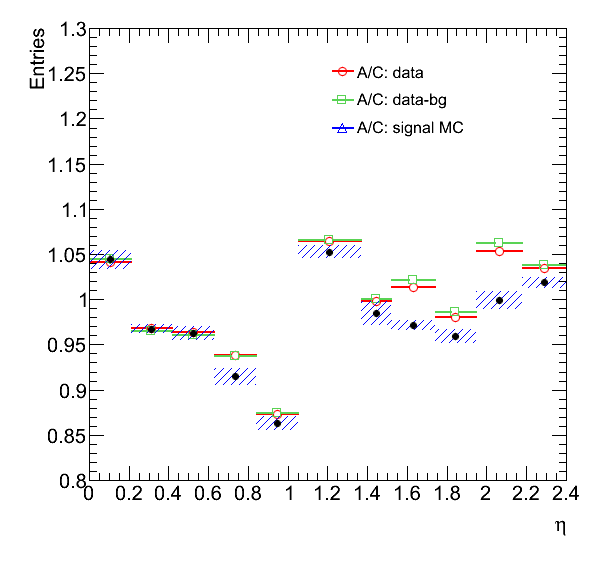
\includegraphics[width=1.0\textwidth]{dates/20130306/figures/wz/W_NOM_Q0_stack_d3_eta_lpt_met_y_2__1_z_0__1_POS}

\column{.5\textwidth}
\centering
\small{ W (nominal), $\mu^{-}$}
\includegraphics[width=1.0\textwidth]<2>{dates/20130306/figures/wz/W_NOM_Q0_stack_d3_eta_lpt_met_y_2__1_z_0__1_NEG}

\cole
}

\only<3> {
\colb[T]

\column{.5\textwidth}
C-side $\mu^{+}$ (top: W; bottom: Z)
\centering
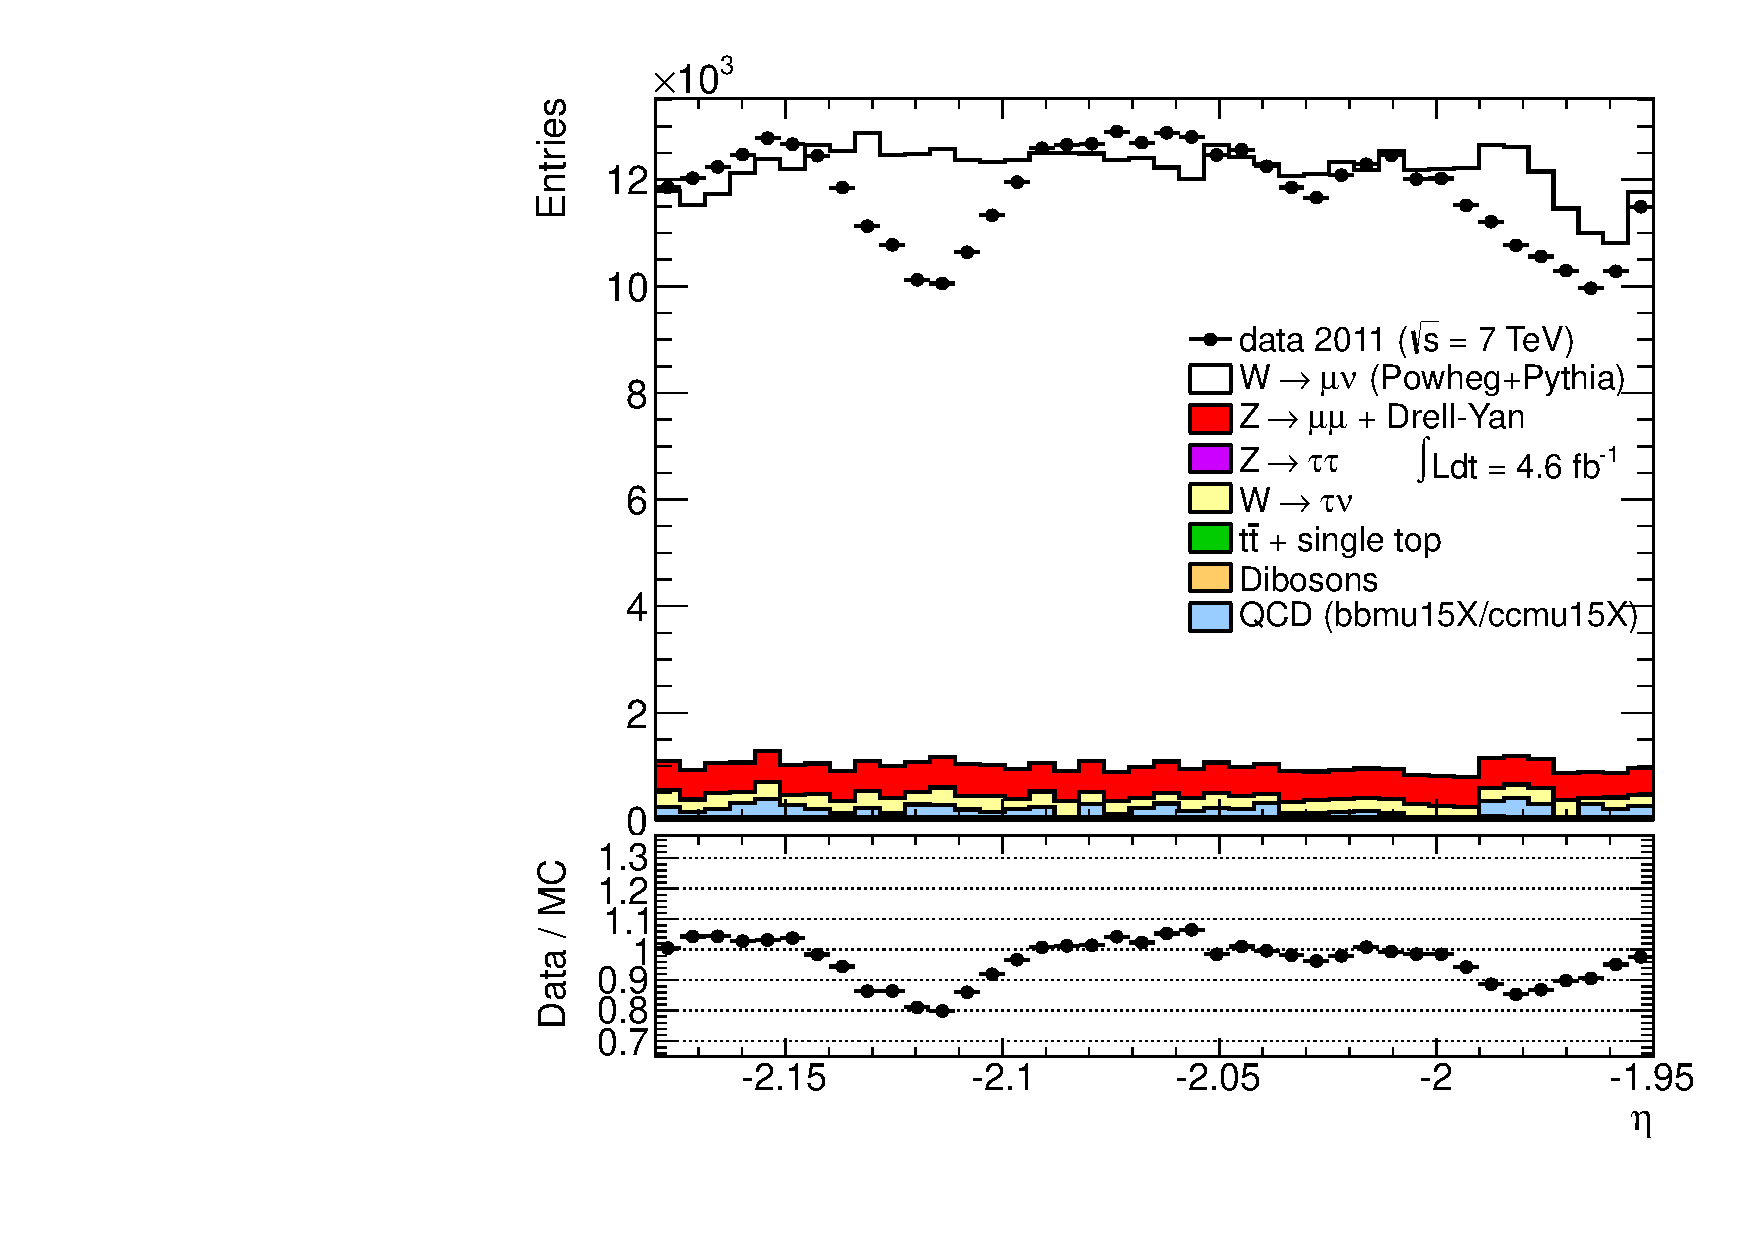
\includegraphics[width=0.66\textwidth]{dates/20130306/figures/etaphi/W_10_C_stack_l_eta_POS} \\
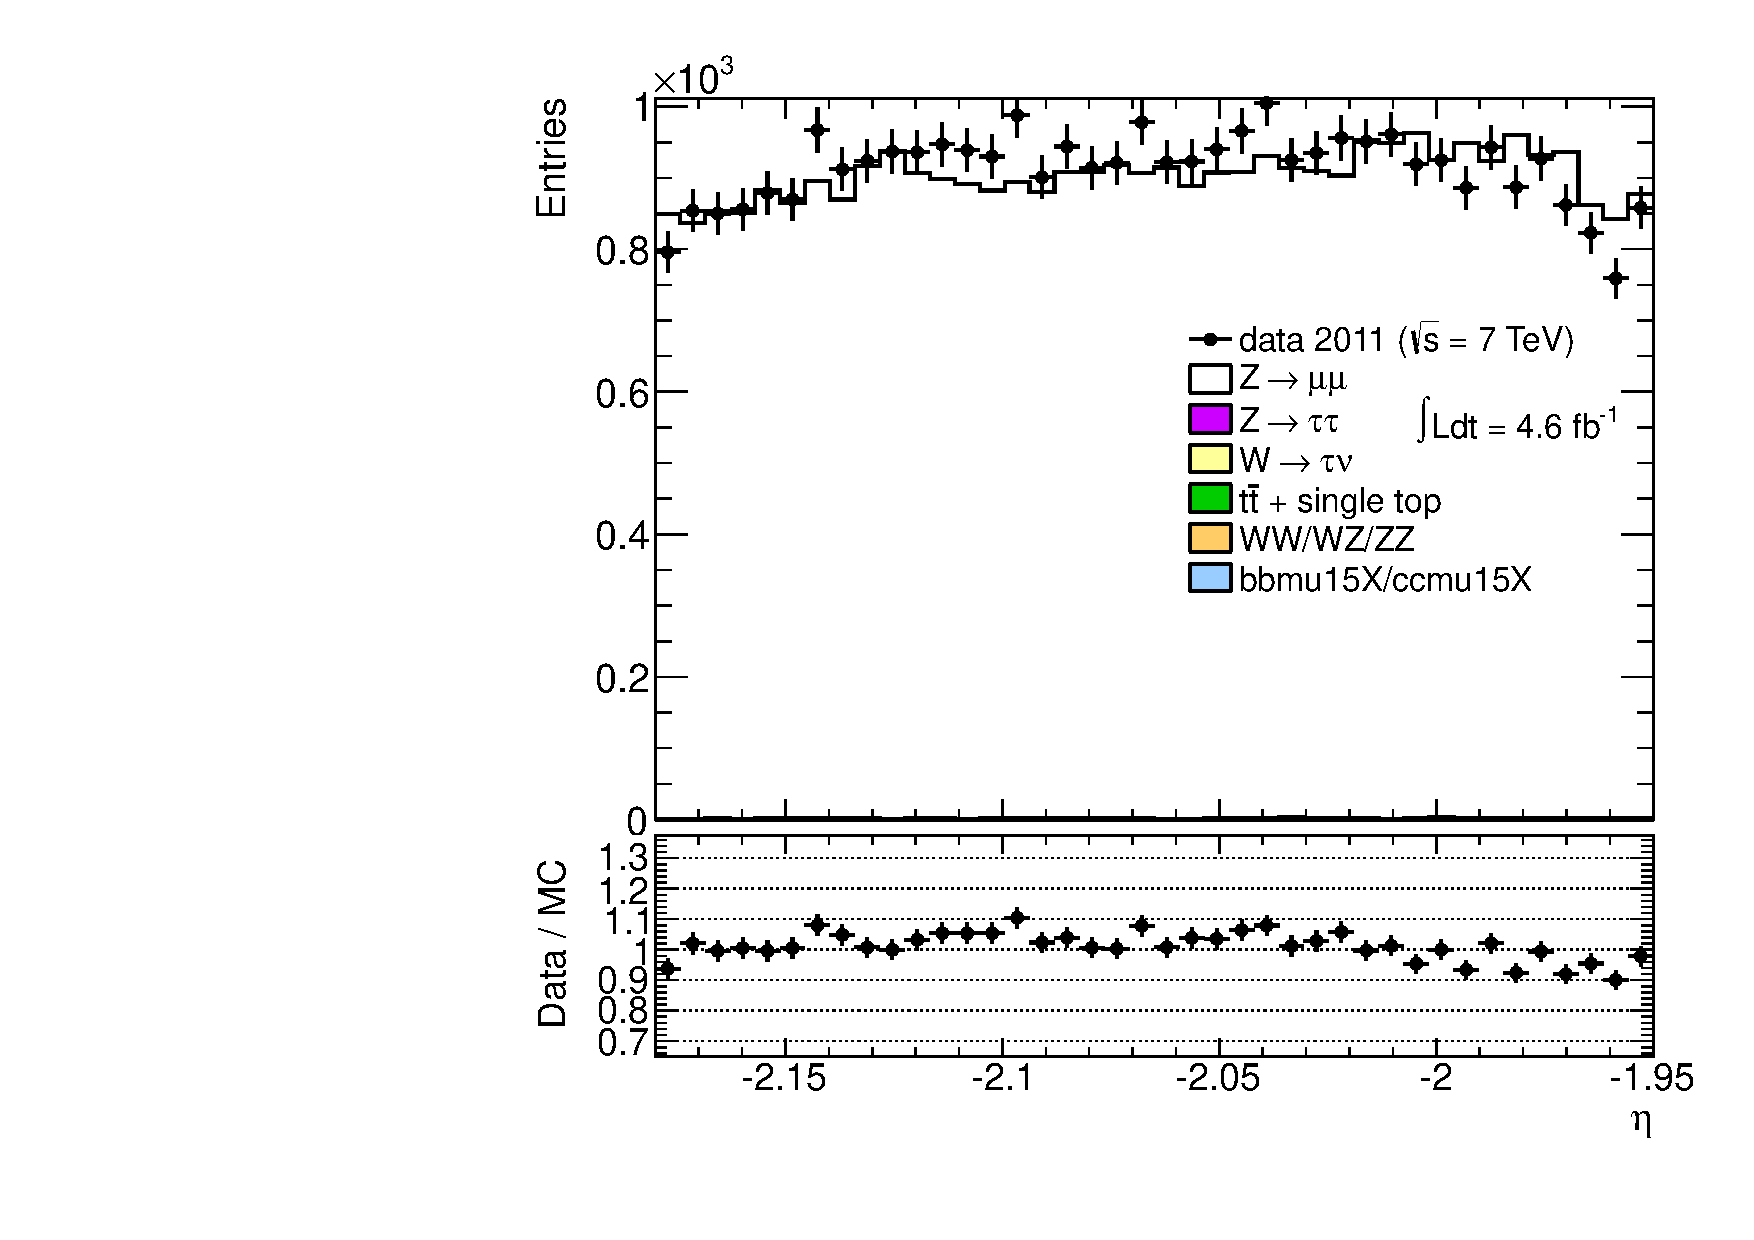
\includegraphics[width=0.66\textwidth]{dates/20130306/figures/etaphi/Z_10_C_stack_lP_eta_ALL.pdf}

\column{.5\textwidth}
A-side $\mu^{+}$ (top: W; bottom: Z)
\centering
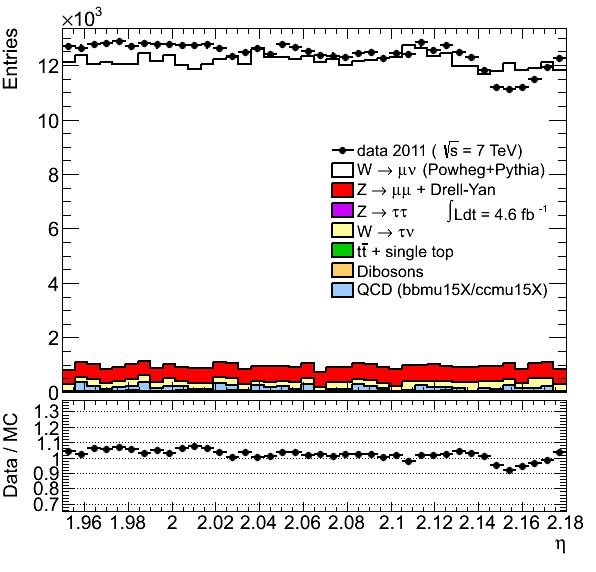
\includegraphics[width=0.66\textwidth]{dates/20130306/figures/etaphi/W_10_A_stack_l_eta_POS} \\
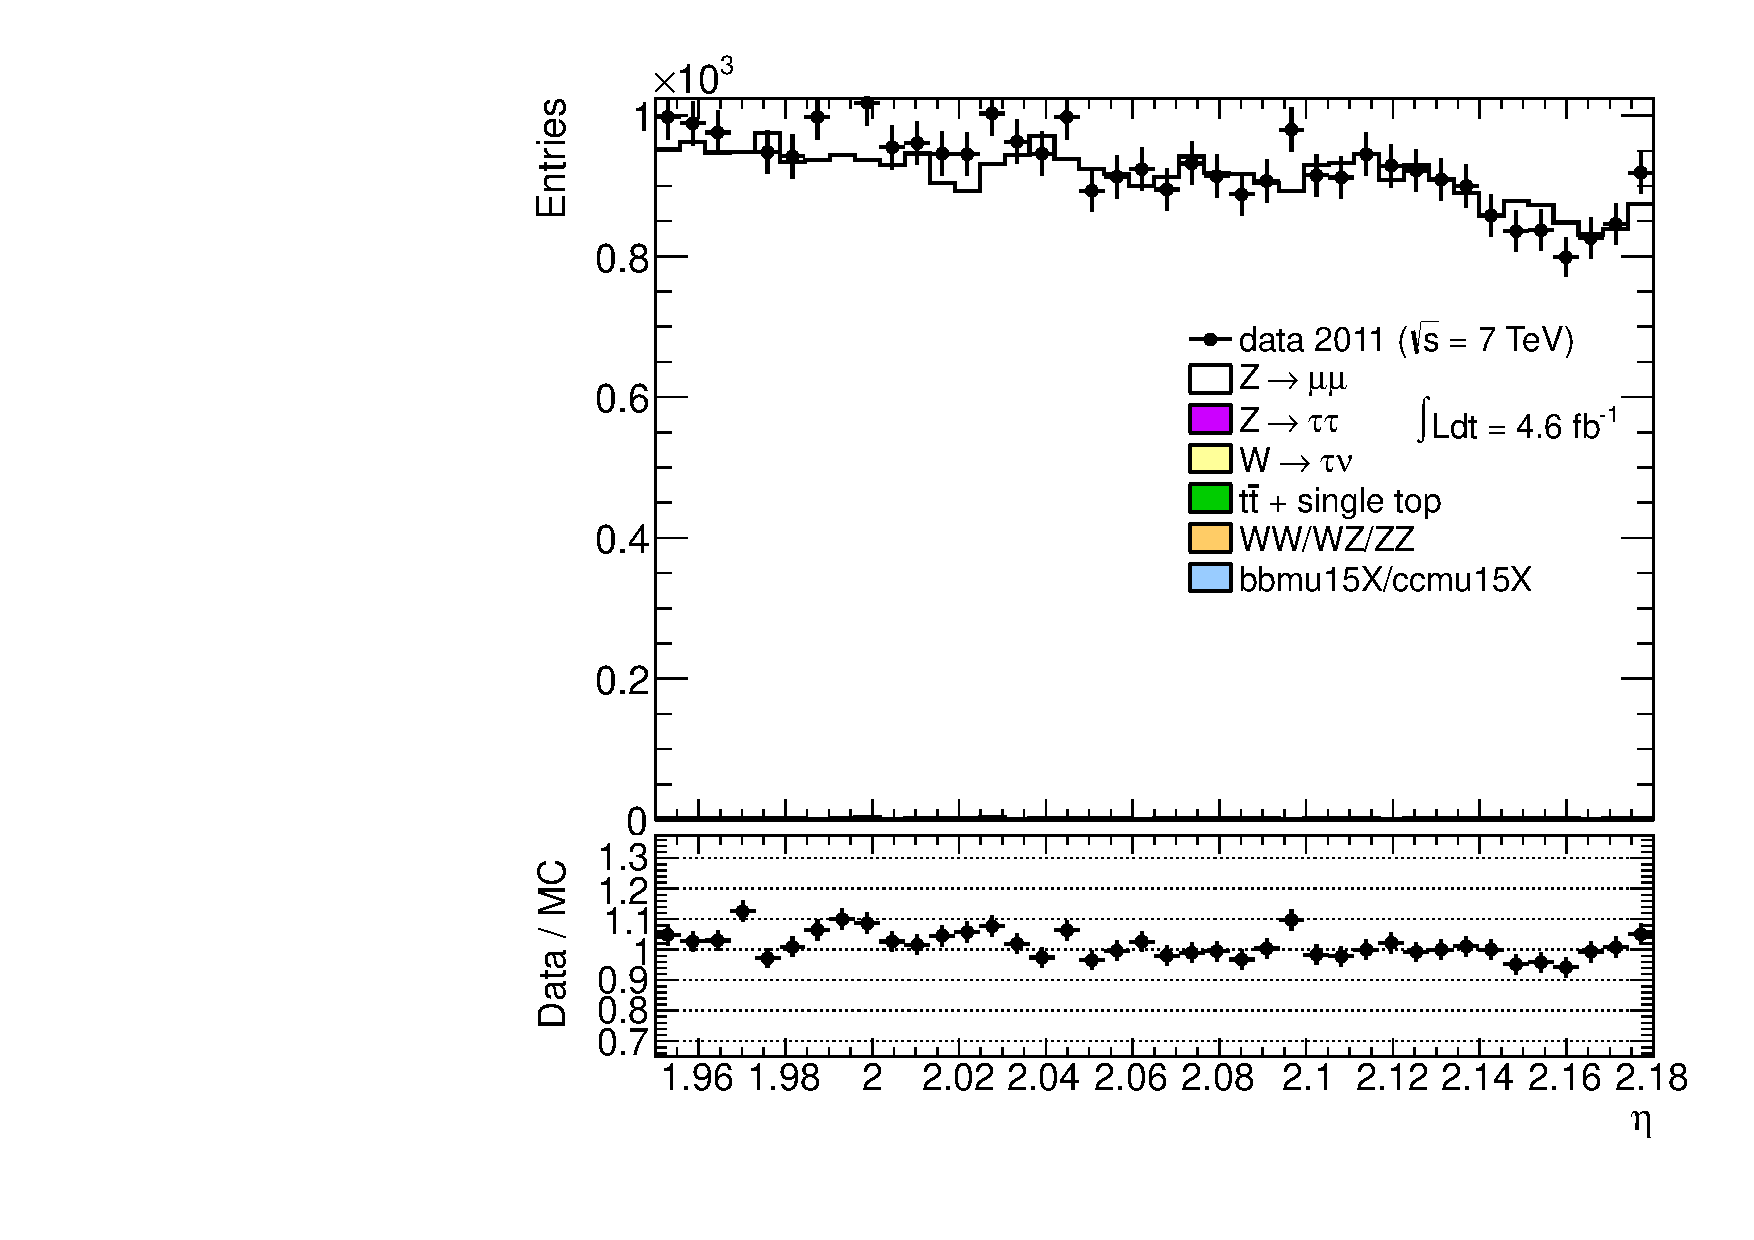
\includegraphics[width=0.66\textwidth]{dates/20130306/figures/etaphi/Z_10_A_stack_lP_eta_ALL.pdf} 

\cole
}

\only<4> {
\colb[T]

\column{.5\textwidth}
C-side $\mu^{-}$ (top: W; bottom: Z)
\centering
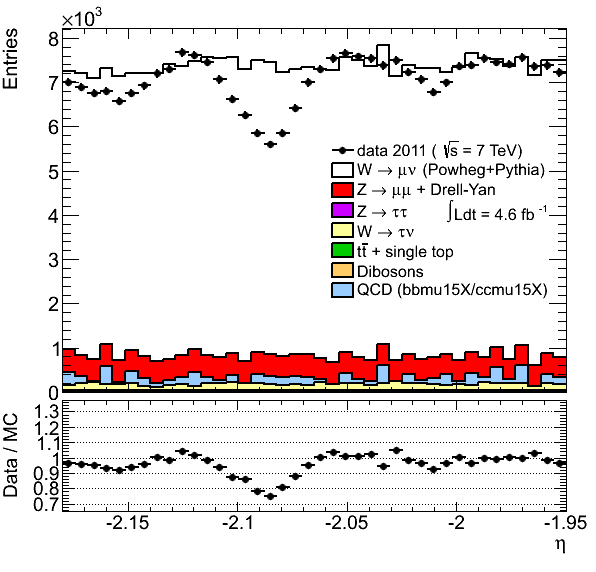
\includegraphics[width=0.66\textwidth]{dates/20130306/figures/etaphi/W_10_C_stack_l_eta_NEG} \\
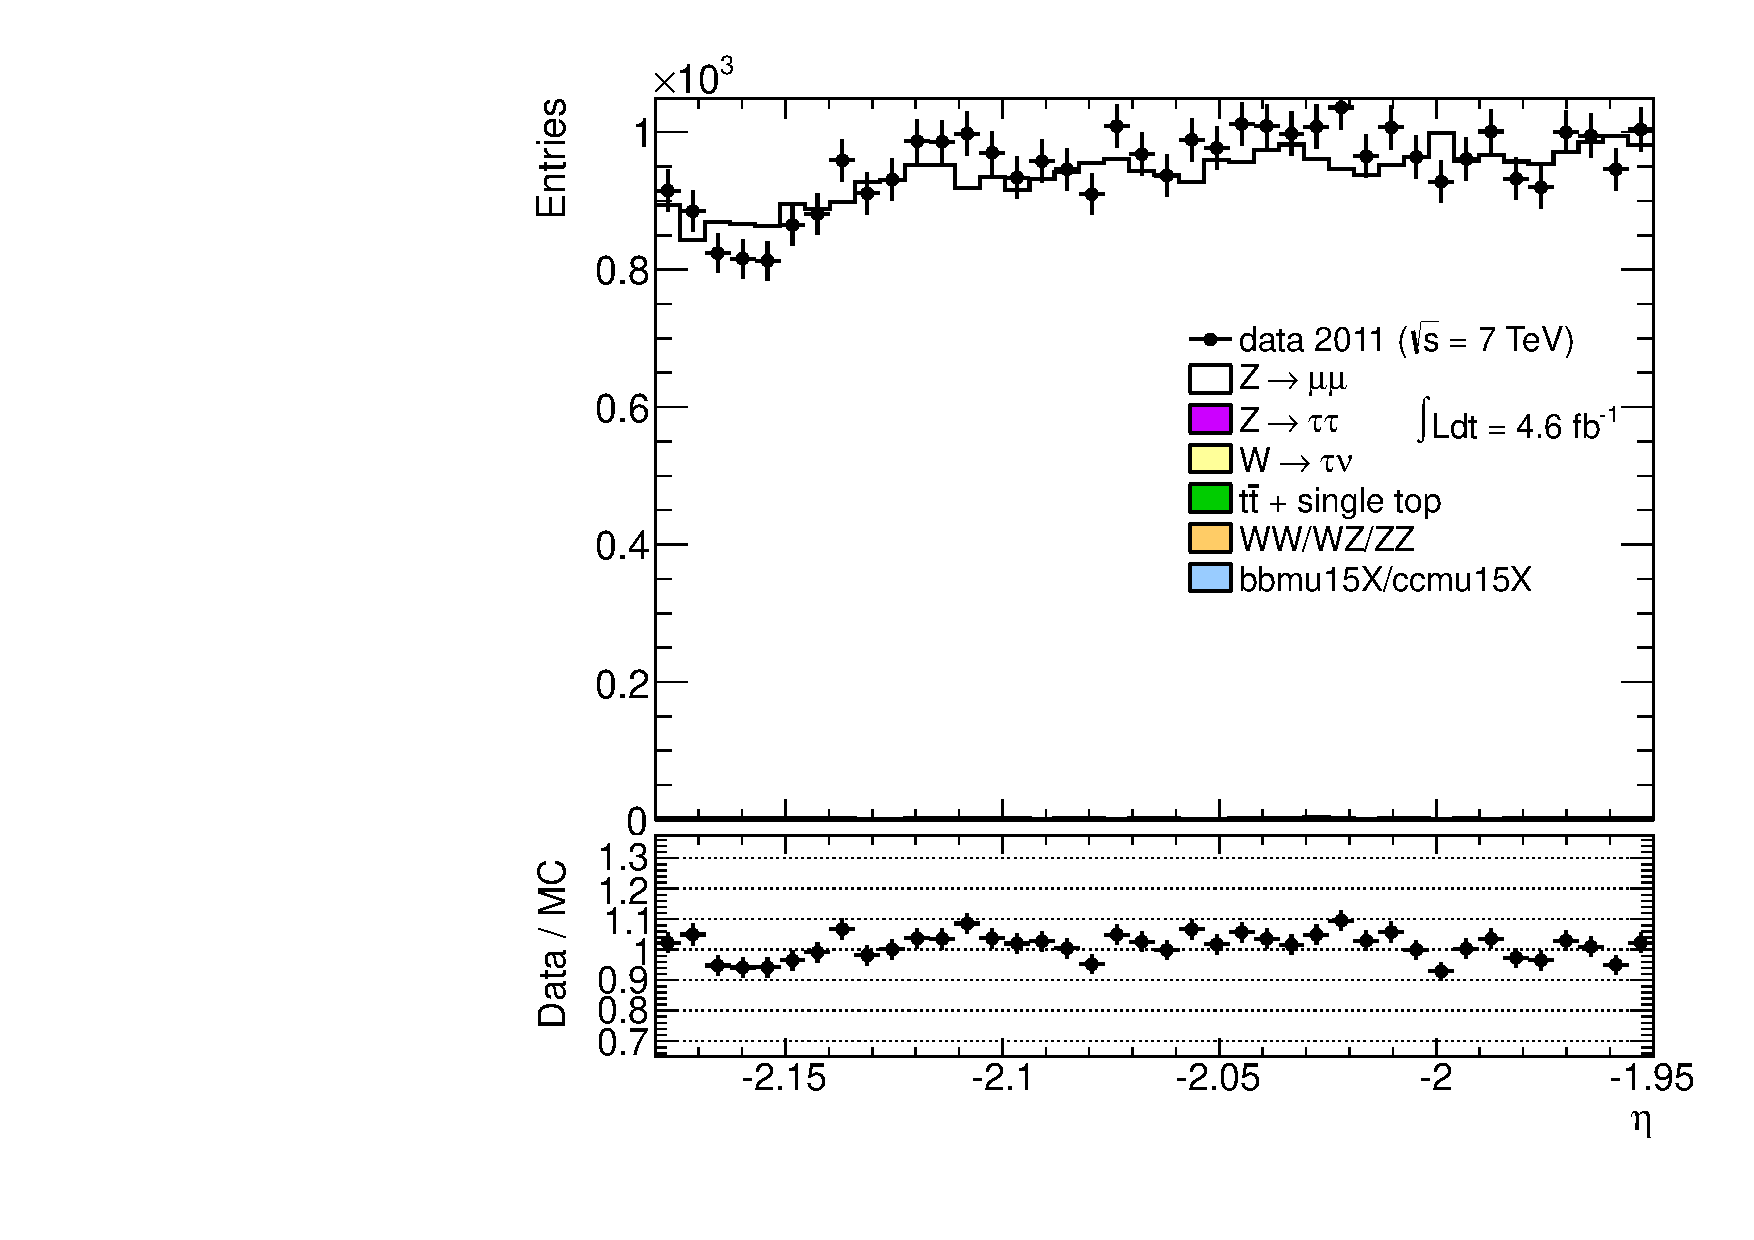
\includegraphics[width=0.66\textwidth]{dates/20130306/figures/etaphi/Z_10_C_stack_lN_eta_ALL.pdf}

\column{.5\textwidth}
A-side $\mu^{-}$ (top: W; bottom: Z)
\centering
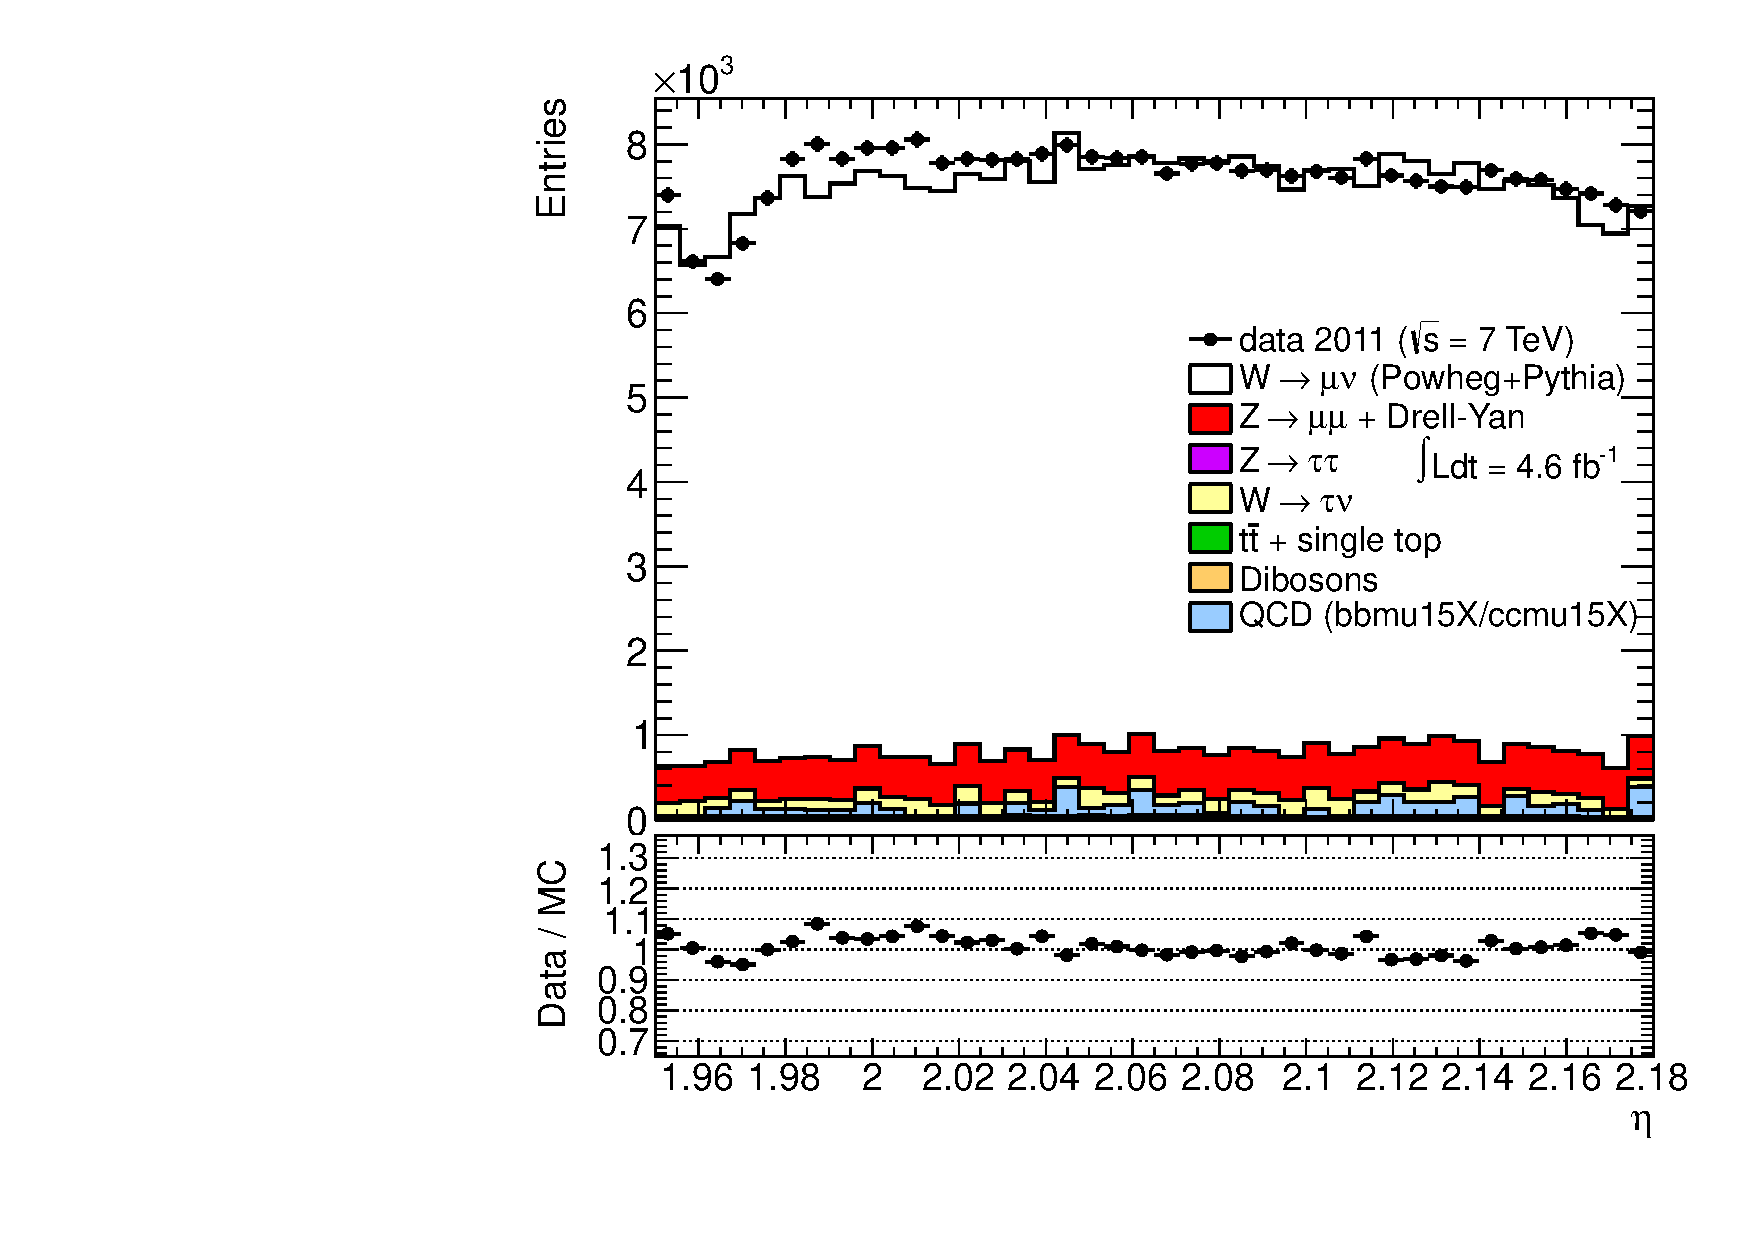
\includegraphics[width=0.66\textwidth]{dates/20130306/figures/etaphi/W_10_A_stack_l_eta_NEG} \\
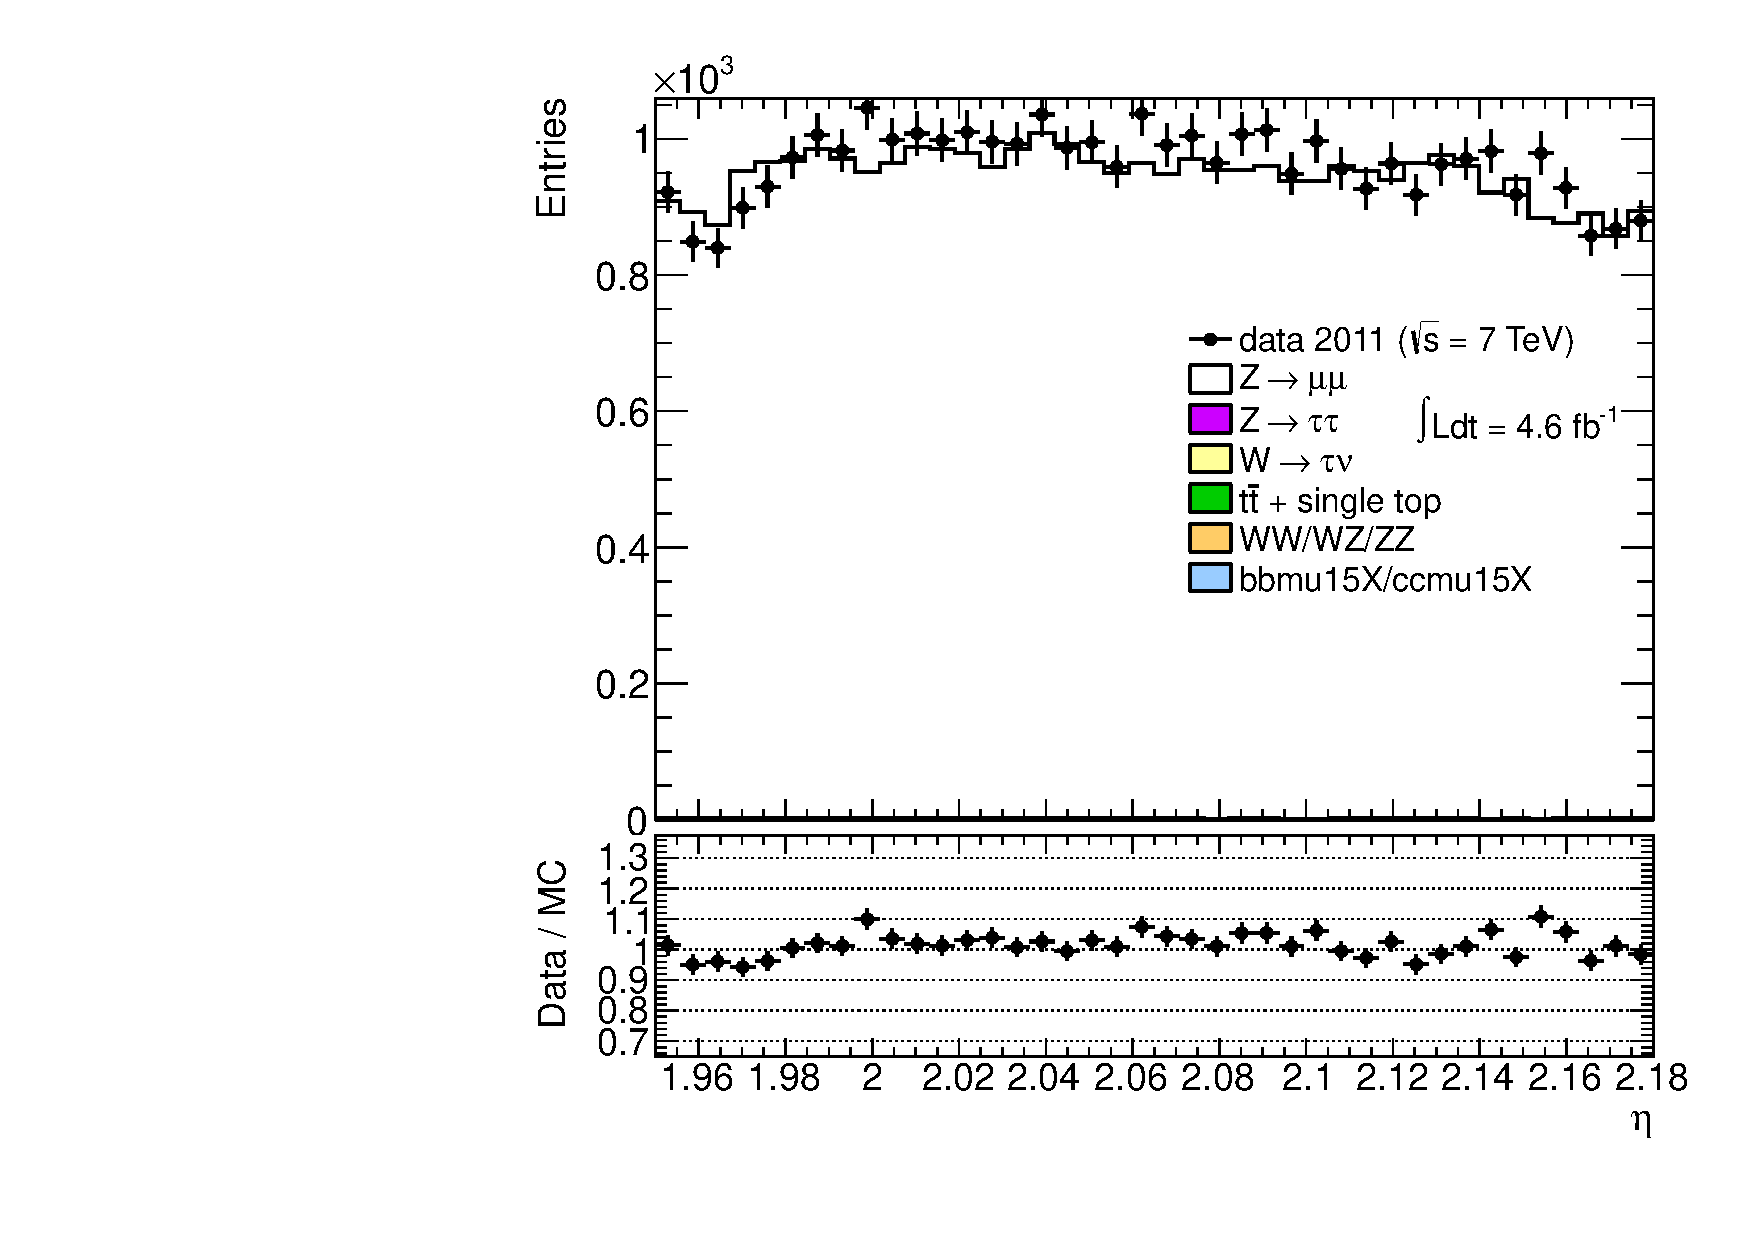
\includegraphics[width=0.66\textwidth]{dates/20130306/figures/etaphi/Z_10_A_stack_lN_eta_ALL.pdf} 

\cole
}

\only<5>{
Well, W has MET. \\
Let's remove MET and WMT cuts from W. \\
(notice enhanced QCD in the W plots)
}

\only<6> {
\colb[T]

\column{.5\textwidth}
C-side $\mu^{-}$ (top: W; bottom: Z)
\centering
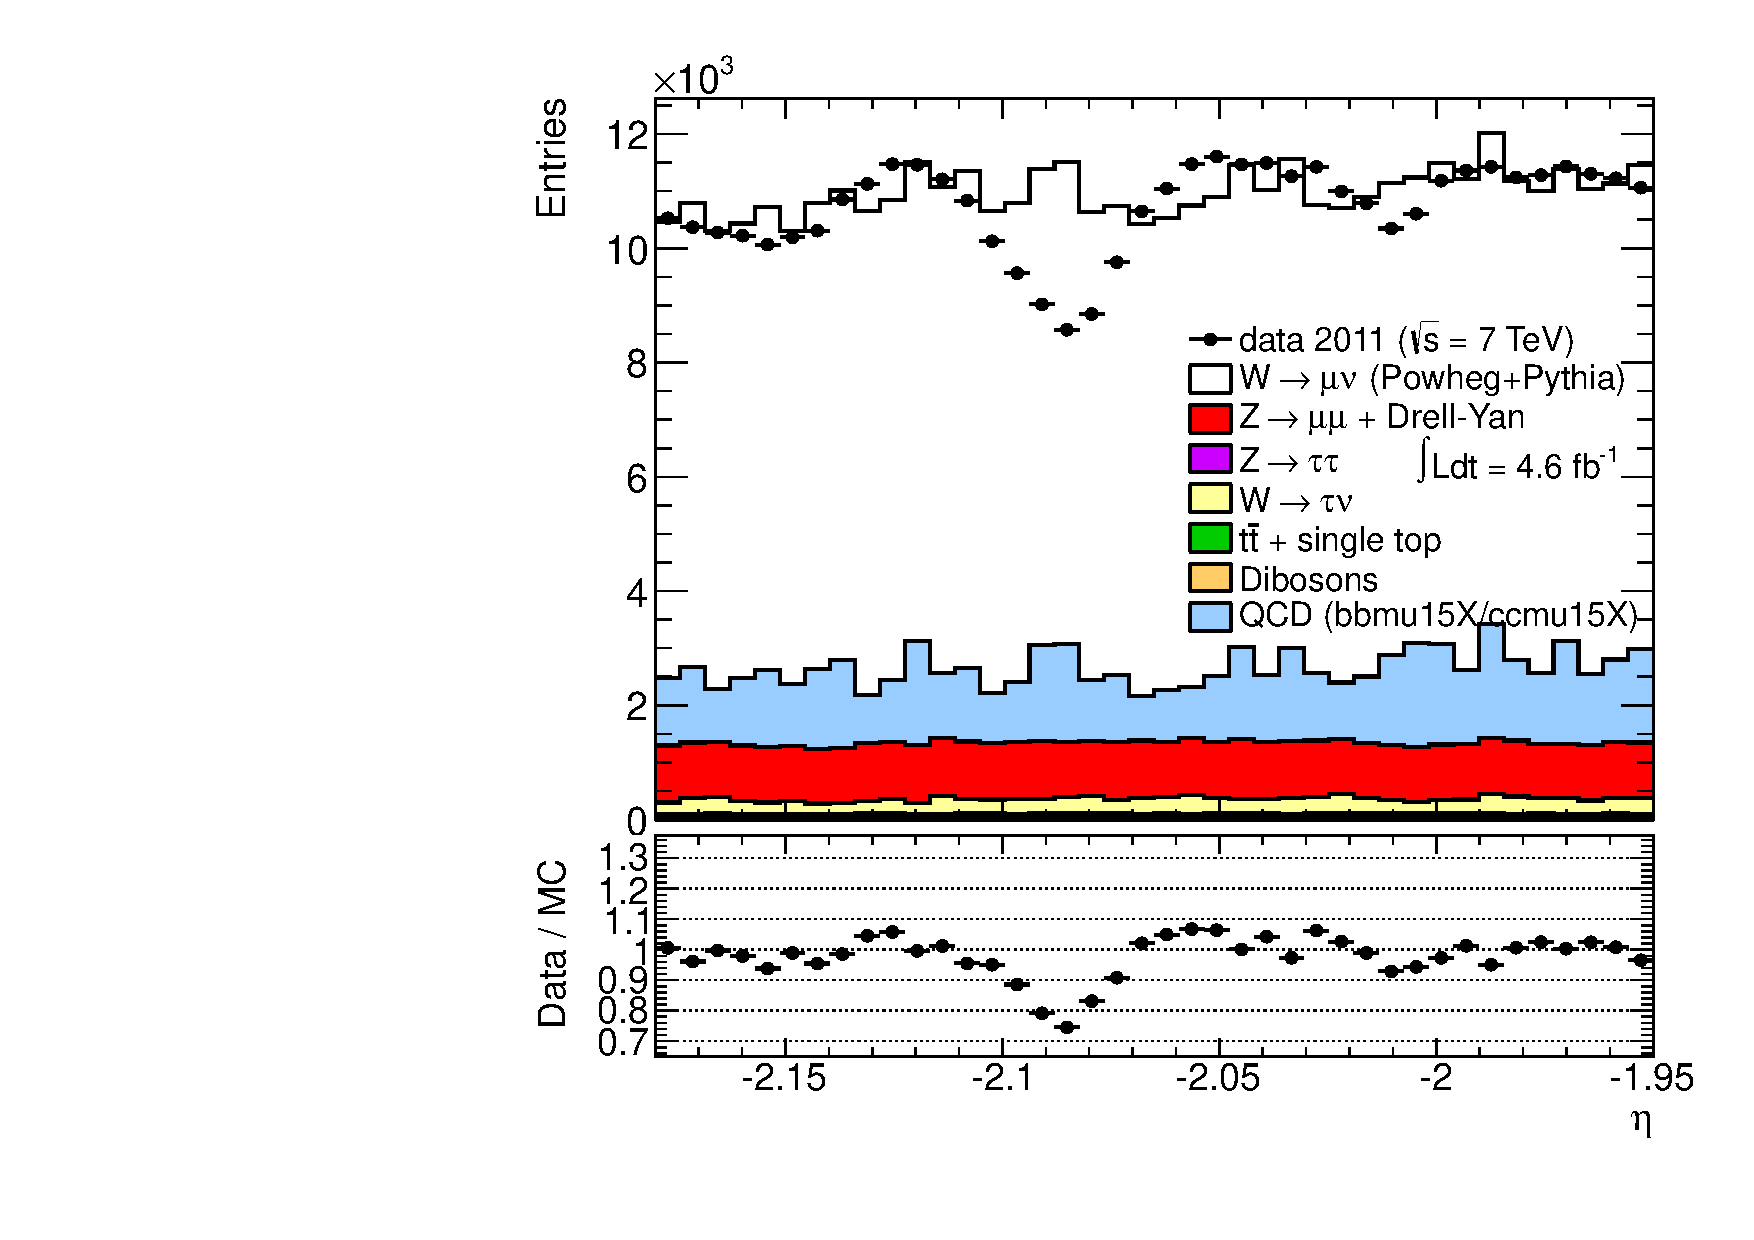
\includegraphics[width=0.66\textwidth]{dates/20130306/figures/etaphi/Wnometmt_10_C_stack_l_eta_NEG} \\
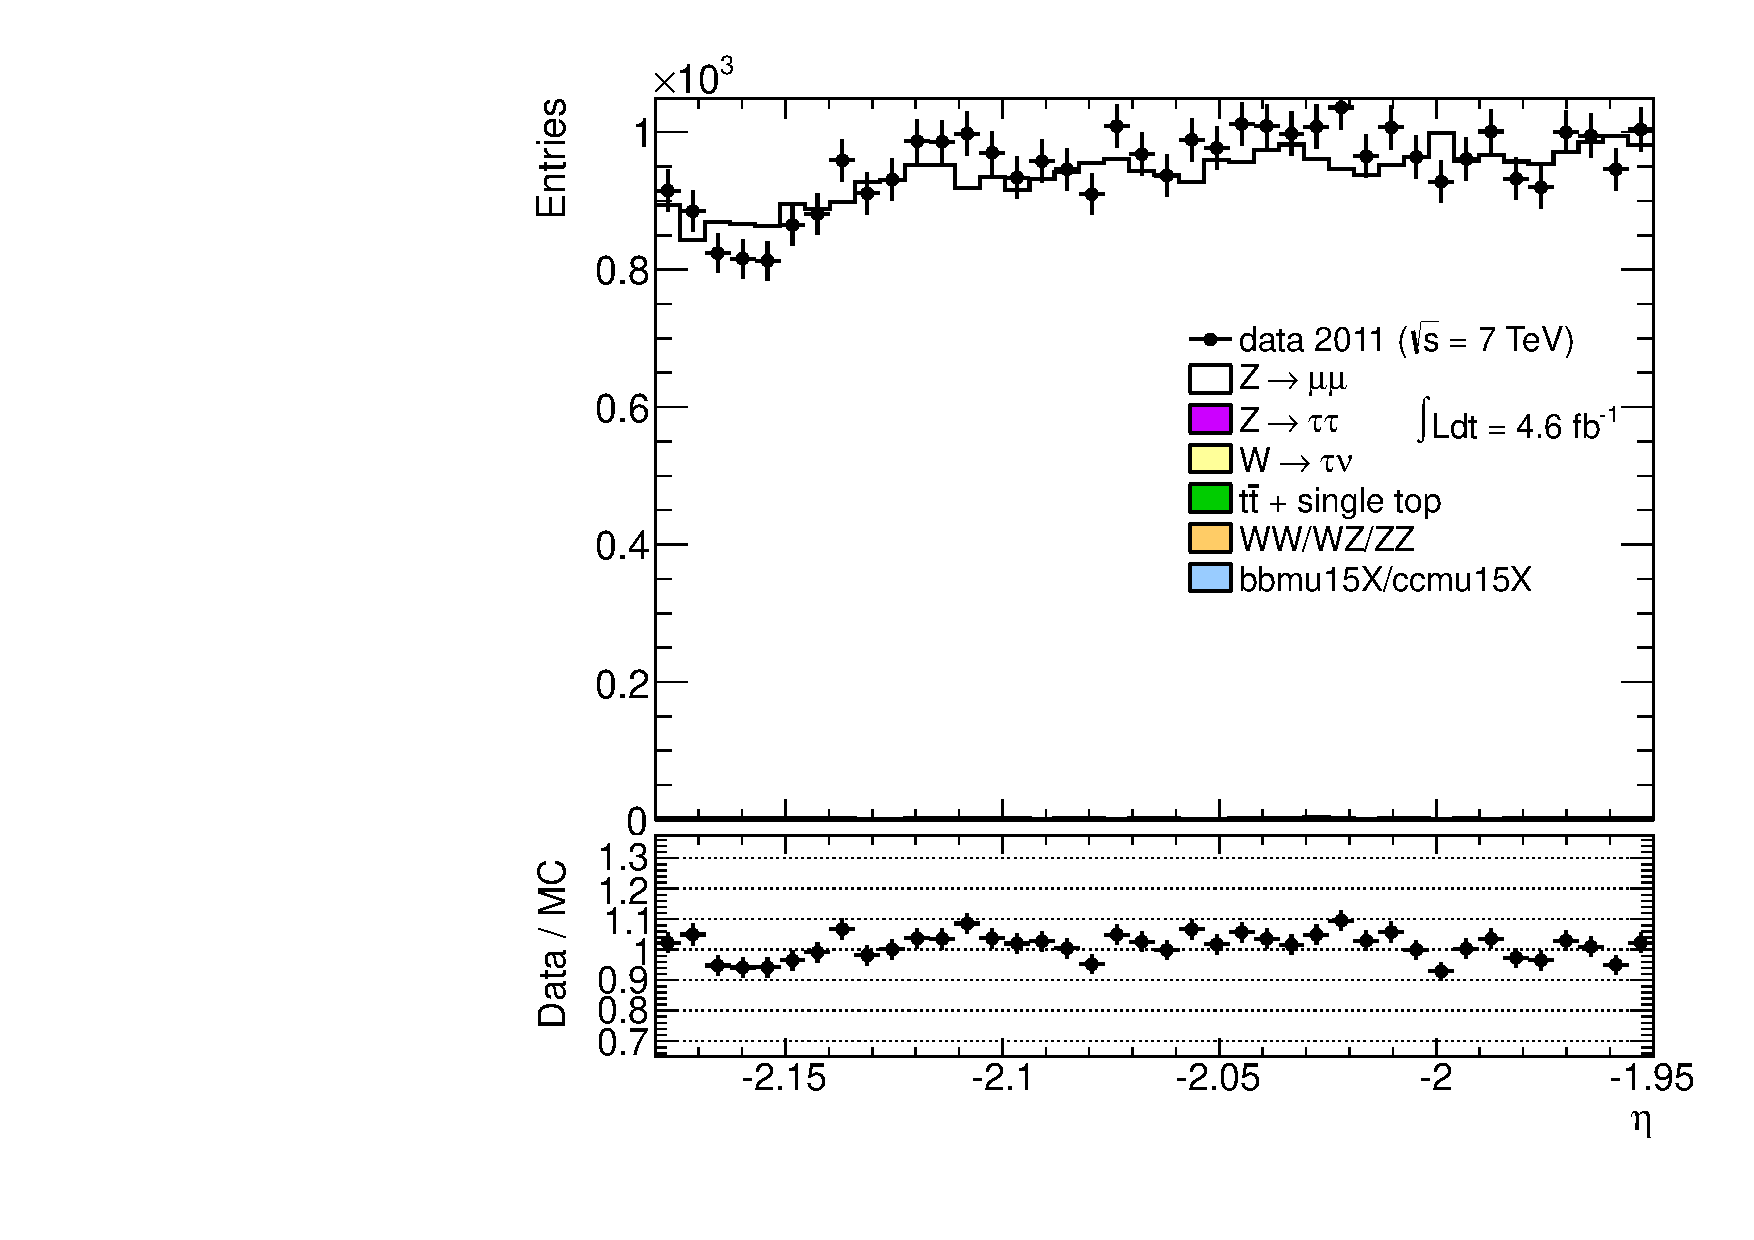
\includegraphics[width=0.66\textwidth]{dates/20130306/figures/etaphi/Z_10_C_stack_lN_eta_ALL.pdf}

\column{.5\textwidth}
A-side $\mu^{-}$ (top: W; bottom: Z)
\centering
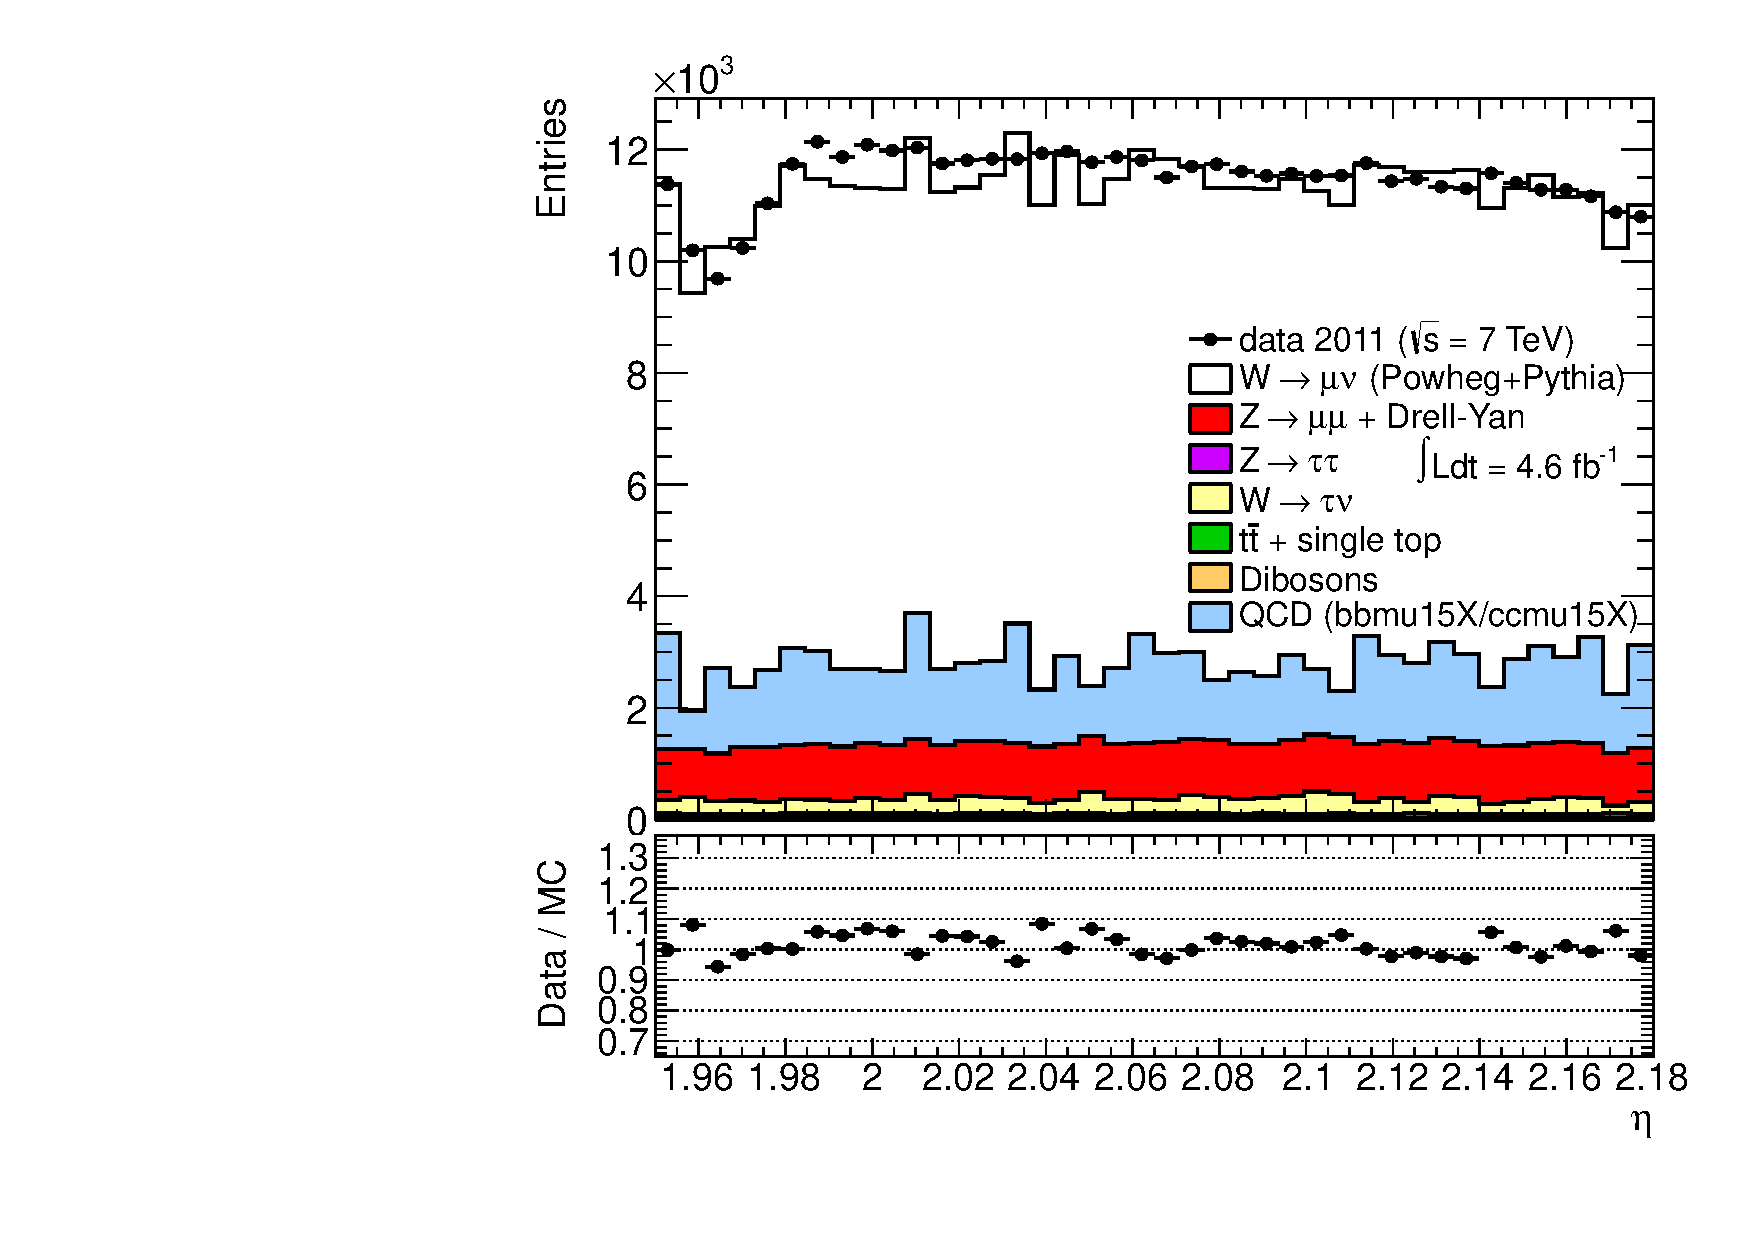
\includegraphics[width=0.66\textwidth]{dates/20130306/figures/etaphi/Wnometmt_10_A_stack_l_eta_NEG} \\
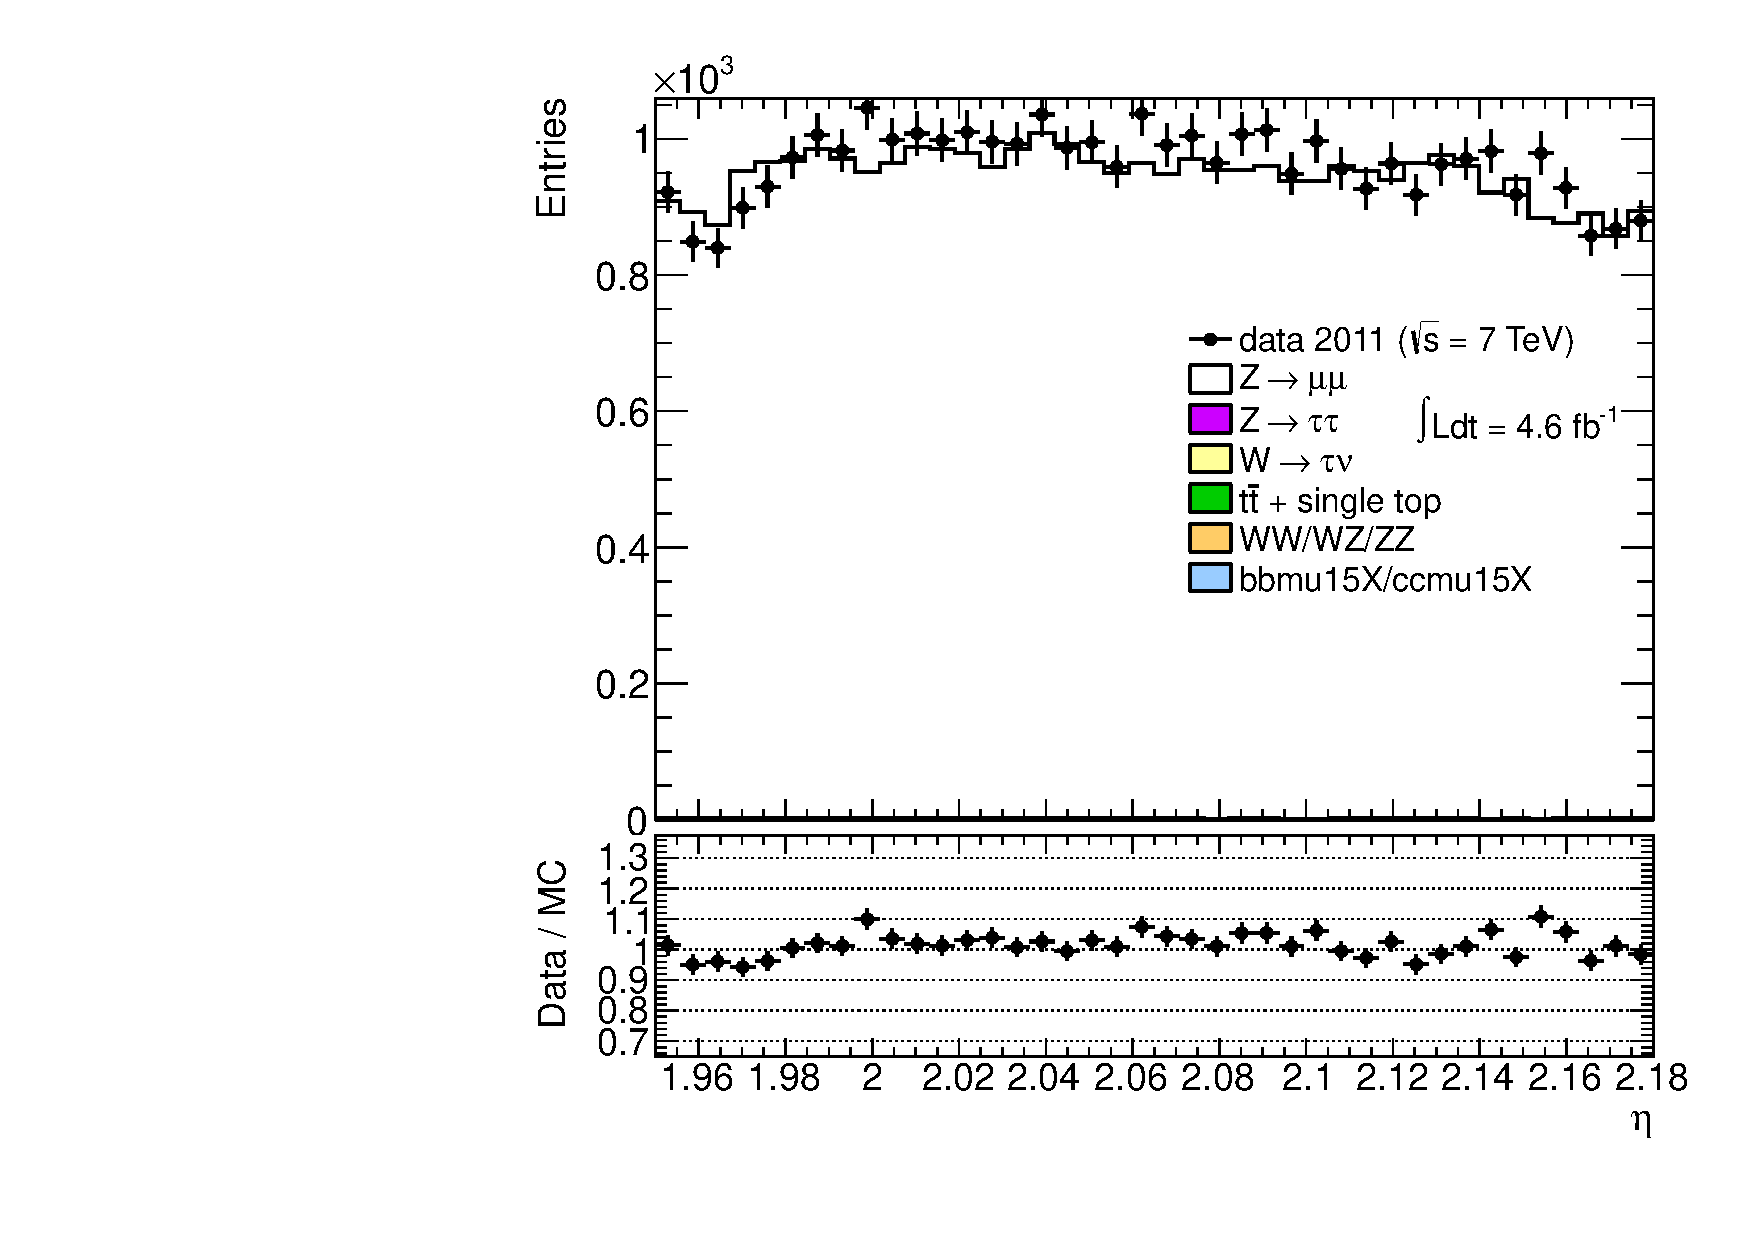
\includegraphics[width=0.66\textwidth]{dates/20130306/figures/etaphi/Z_10_A_stack_lN_eta_ALL.pdf} 

\cole
}

\only<7>{
Z boson is a little heavier and may give off more energetic muons. \\
What if the lower-pT muons in the W channel produce the dip? \\
Let's try to bump up pT cut to 35 GeV on both W and Z muons.
}

\only<8> {
\colb[T]

\column{.5\textwidth}
C-side $\mu^{-}$ (top: W; bottom: Z)
\centering
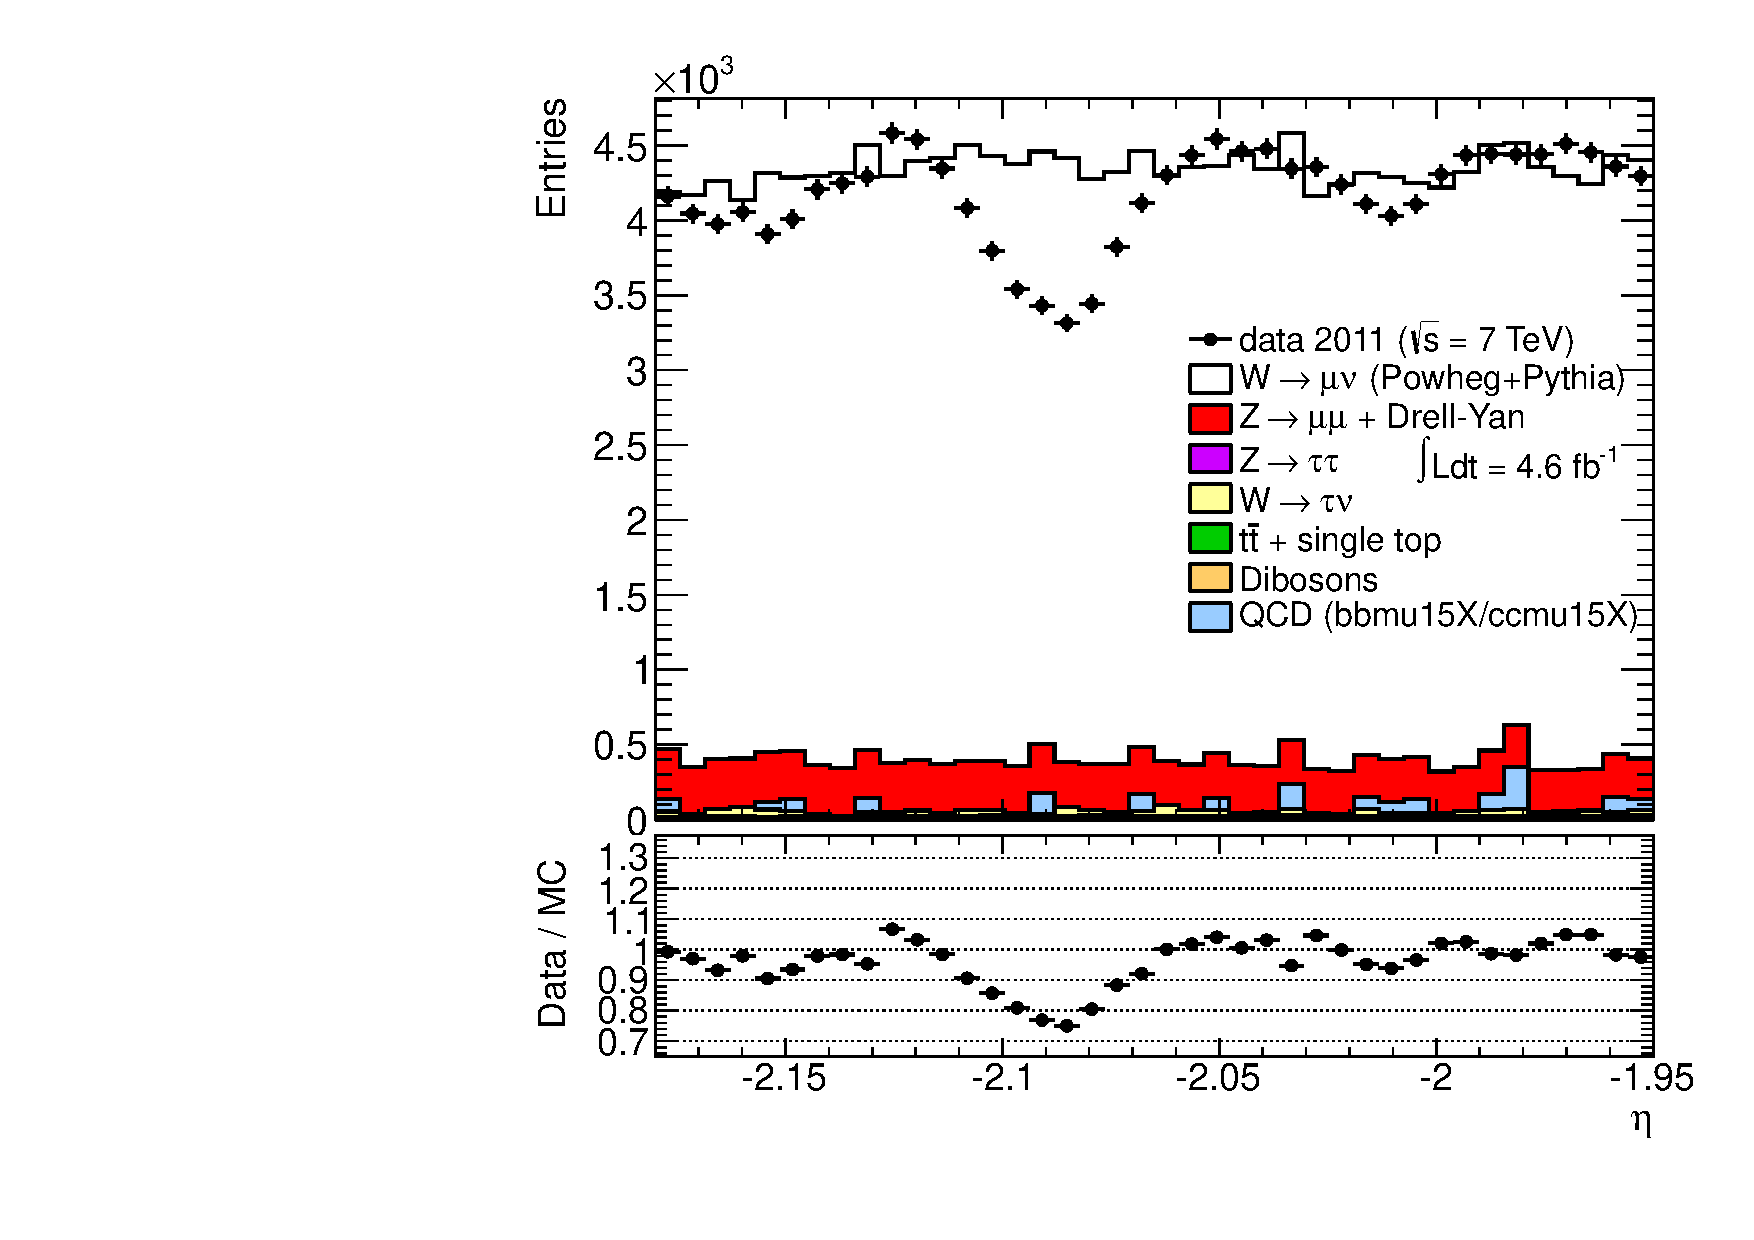
\includegraphics[width=0.66\textwidth]{dates/20130306/figures/etaphi/Wpt35_10_C_stack_l_eta_NEG} \\
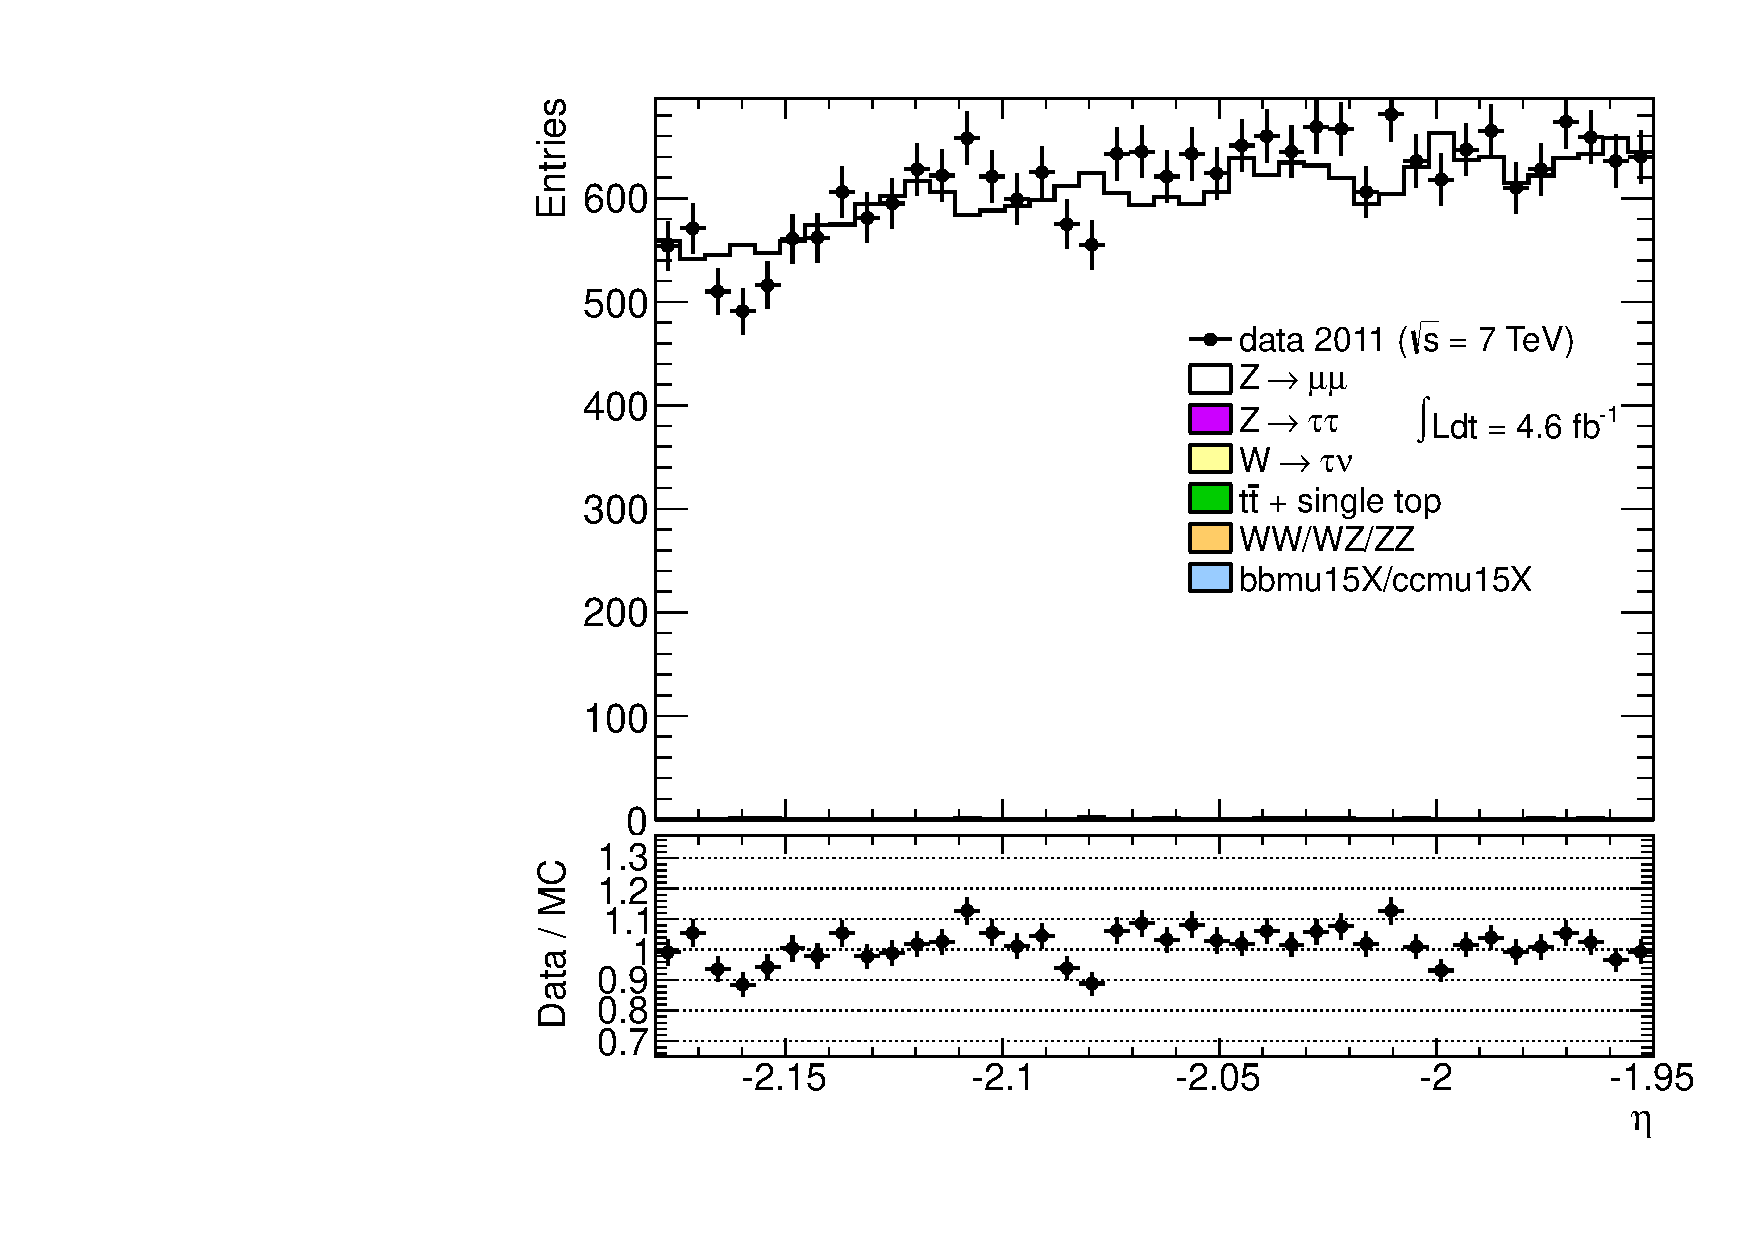
\includegraphics[width=0.66\textwidth]{dates/20130306/figures/etaphi/Zpt35_10_C_stack_lN_eta_ALL.pdf}

\column{.5\textwidth}
A-side $\mu^{-}$ (top: W; bottom: Z)
\centering
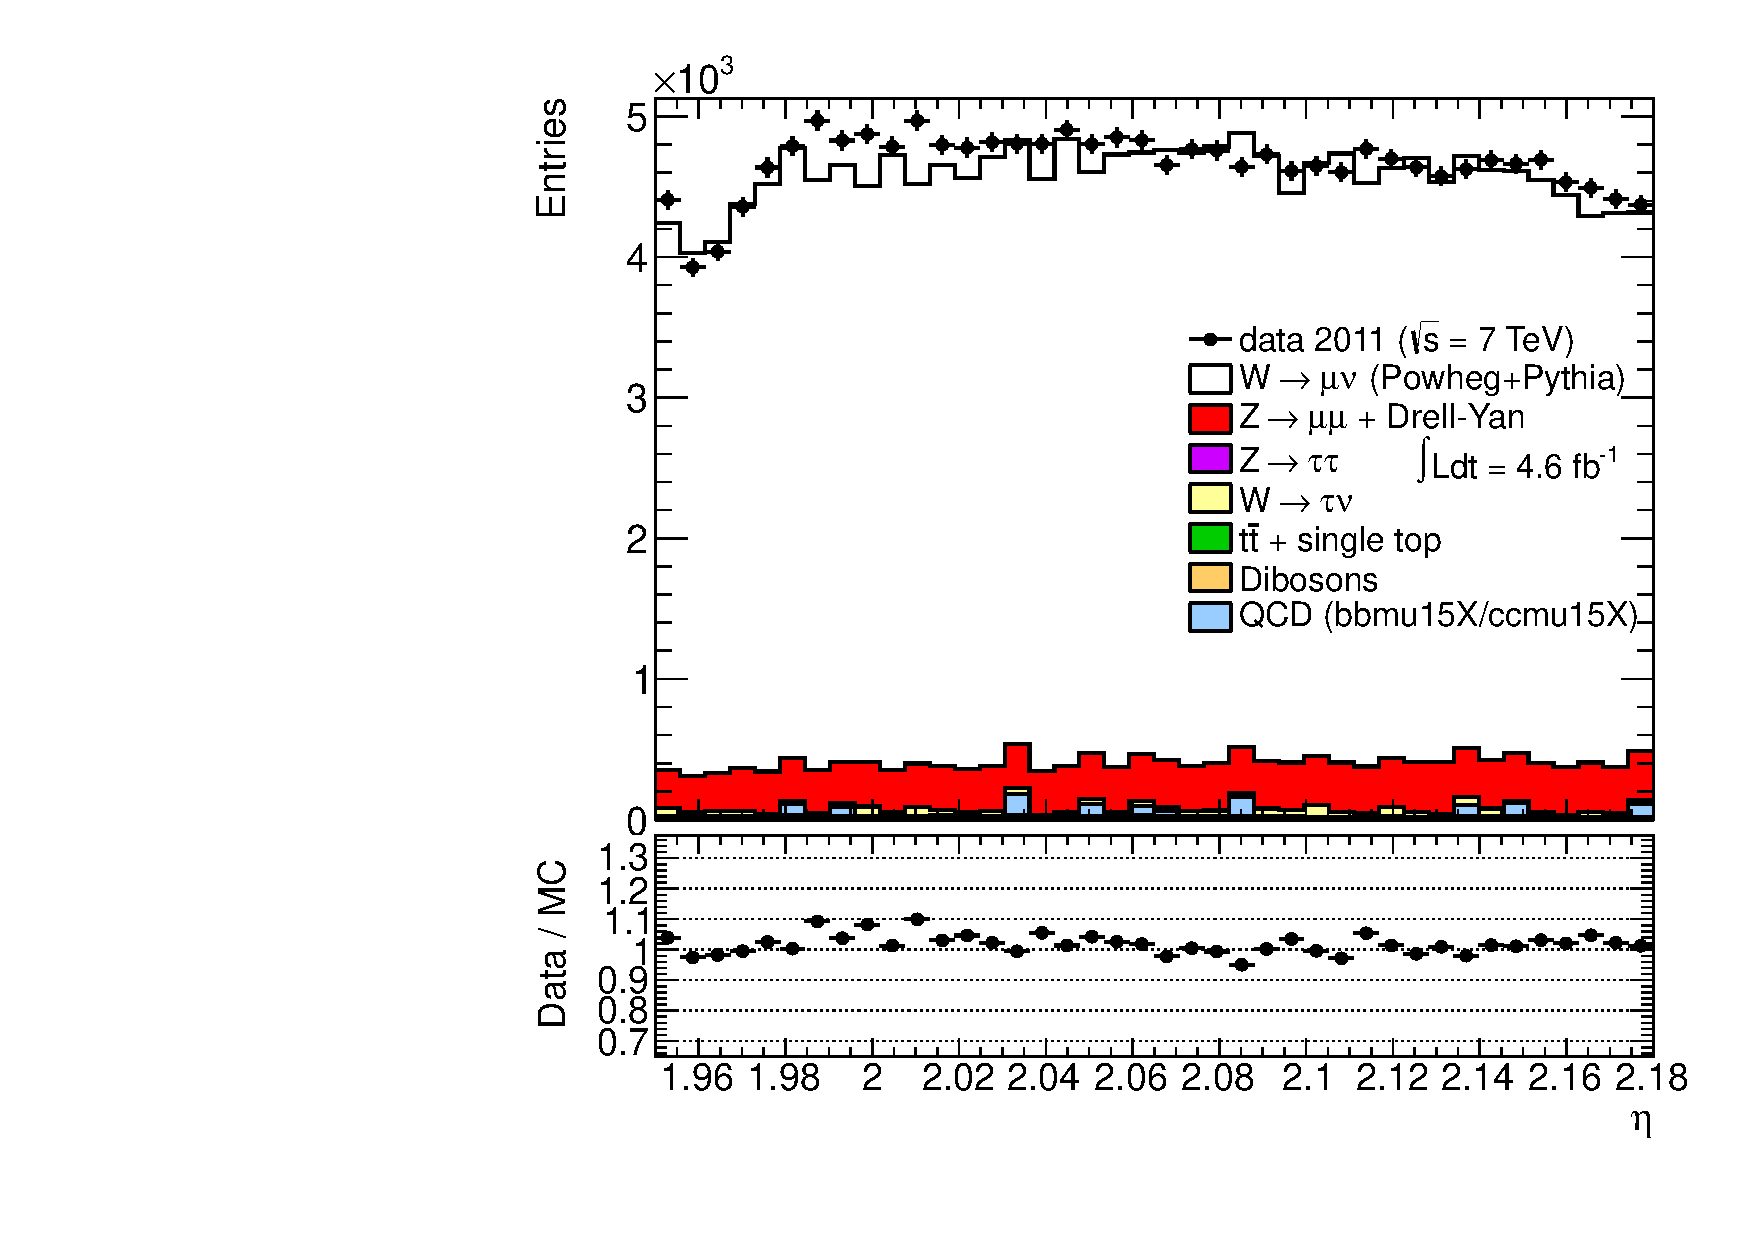
\includegraphics[width=0.66\textwidth]{dates/20130306/figures/etaphi/Wpt35_10_A_stack_l_eta_NEG} \\
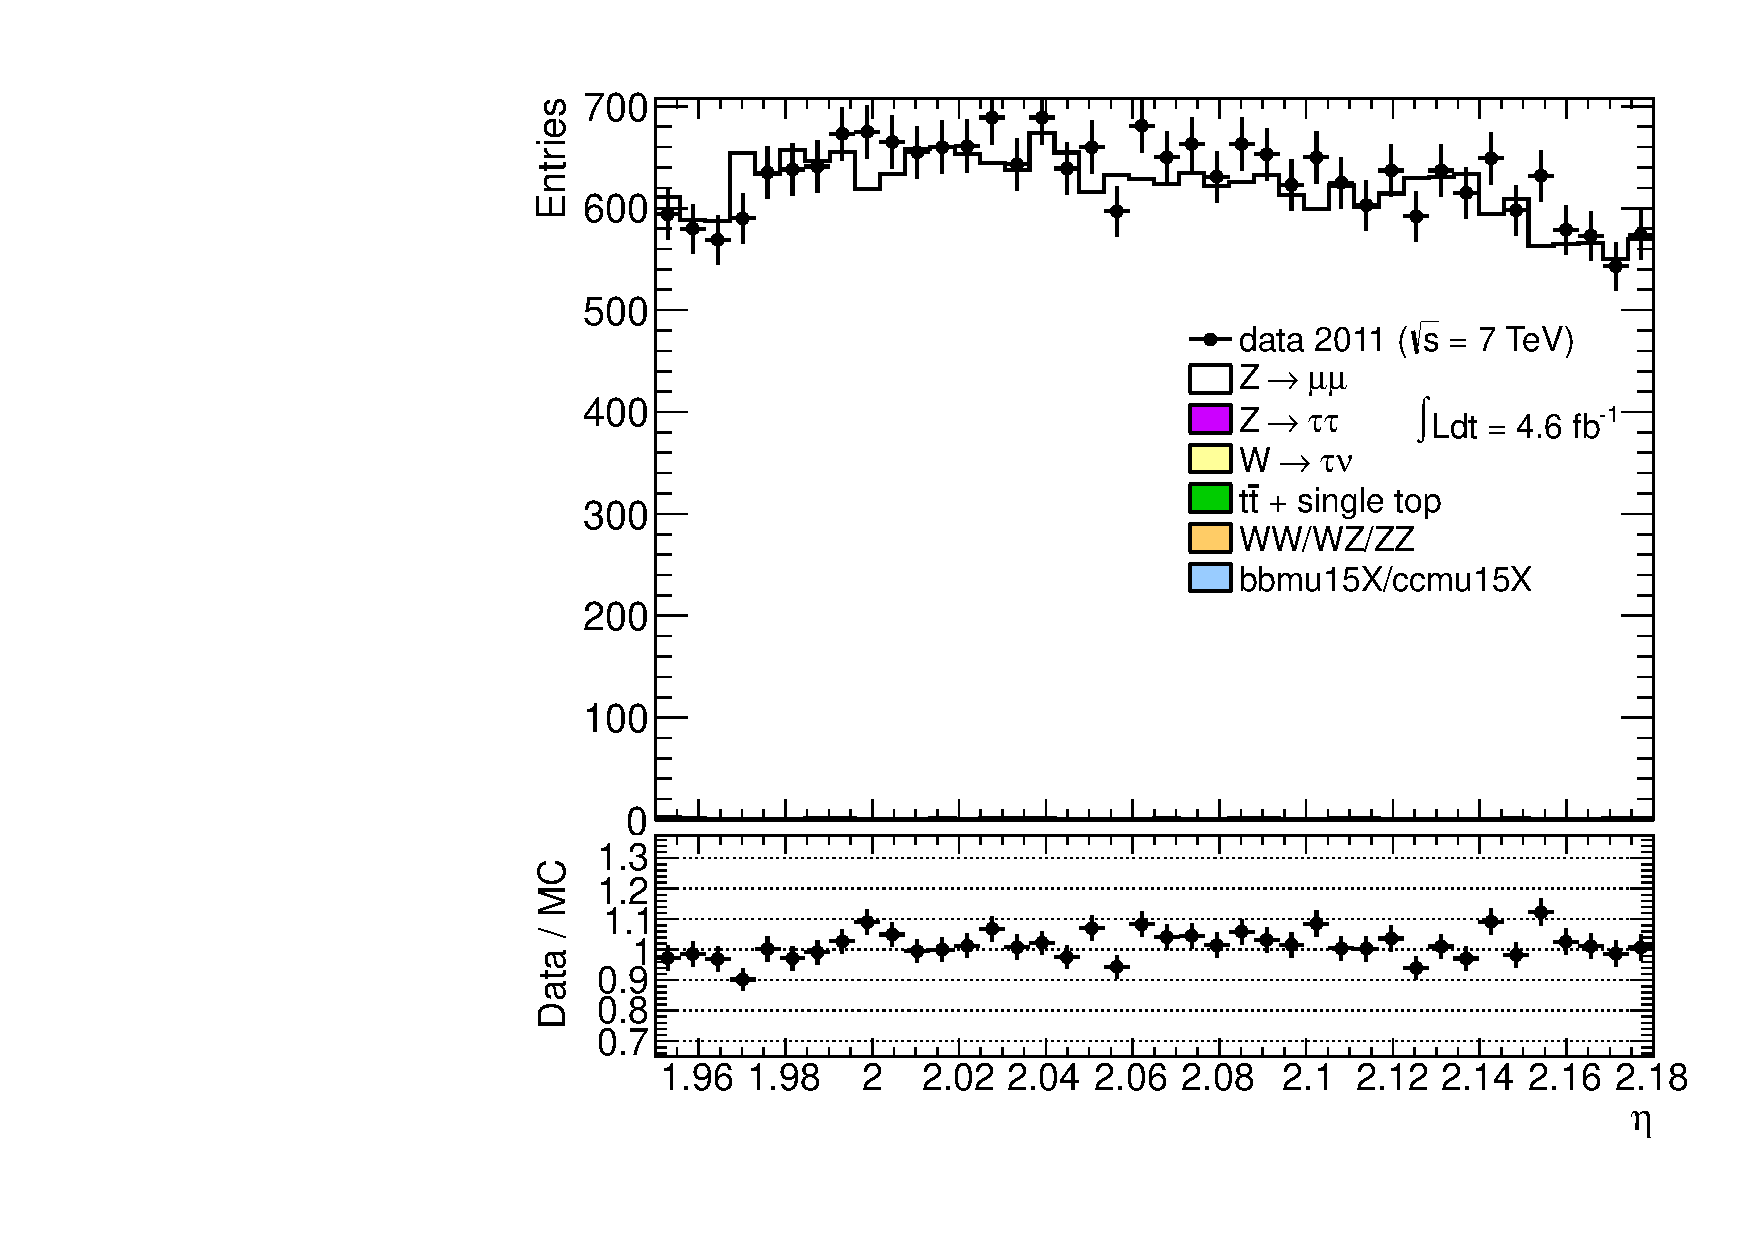
\includegraphics[width=0.66\textwidth]{dates/20130306/figures/etaphi/Zpt35_10_A_stack_lN_eta_ALL.pdf} 

\cole
}

\only<9>{
For completeness, let's try to put an upper cap on pT: \\
Limit pT range to 25-35 GeV for both W and Z muons
}

\only<10> {
\colb[T]

\column{.5\textwidth}
C-side $\mu^{-}$ (top: W; bottom: Z)
\centering
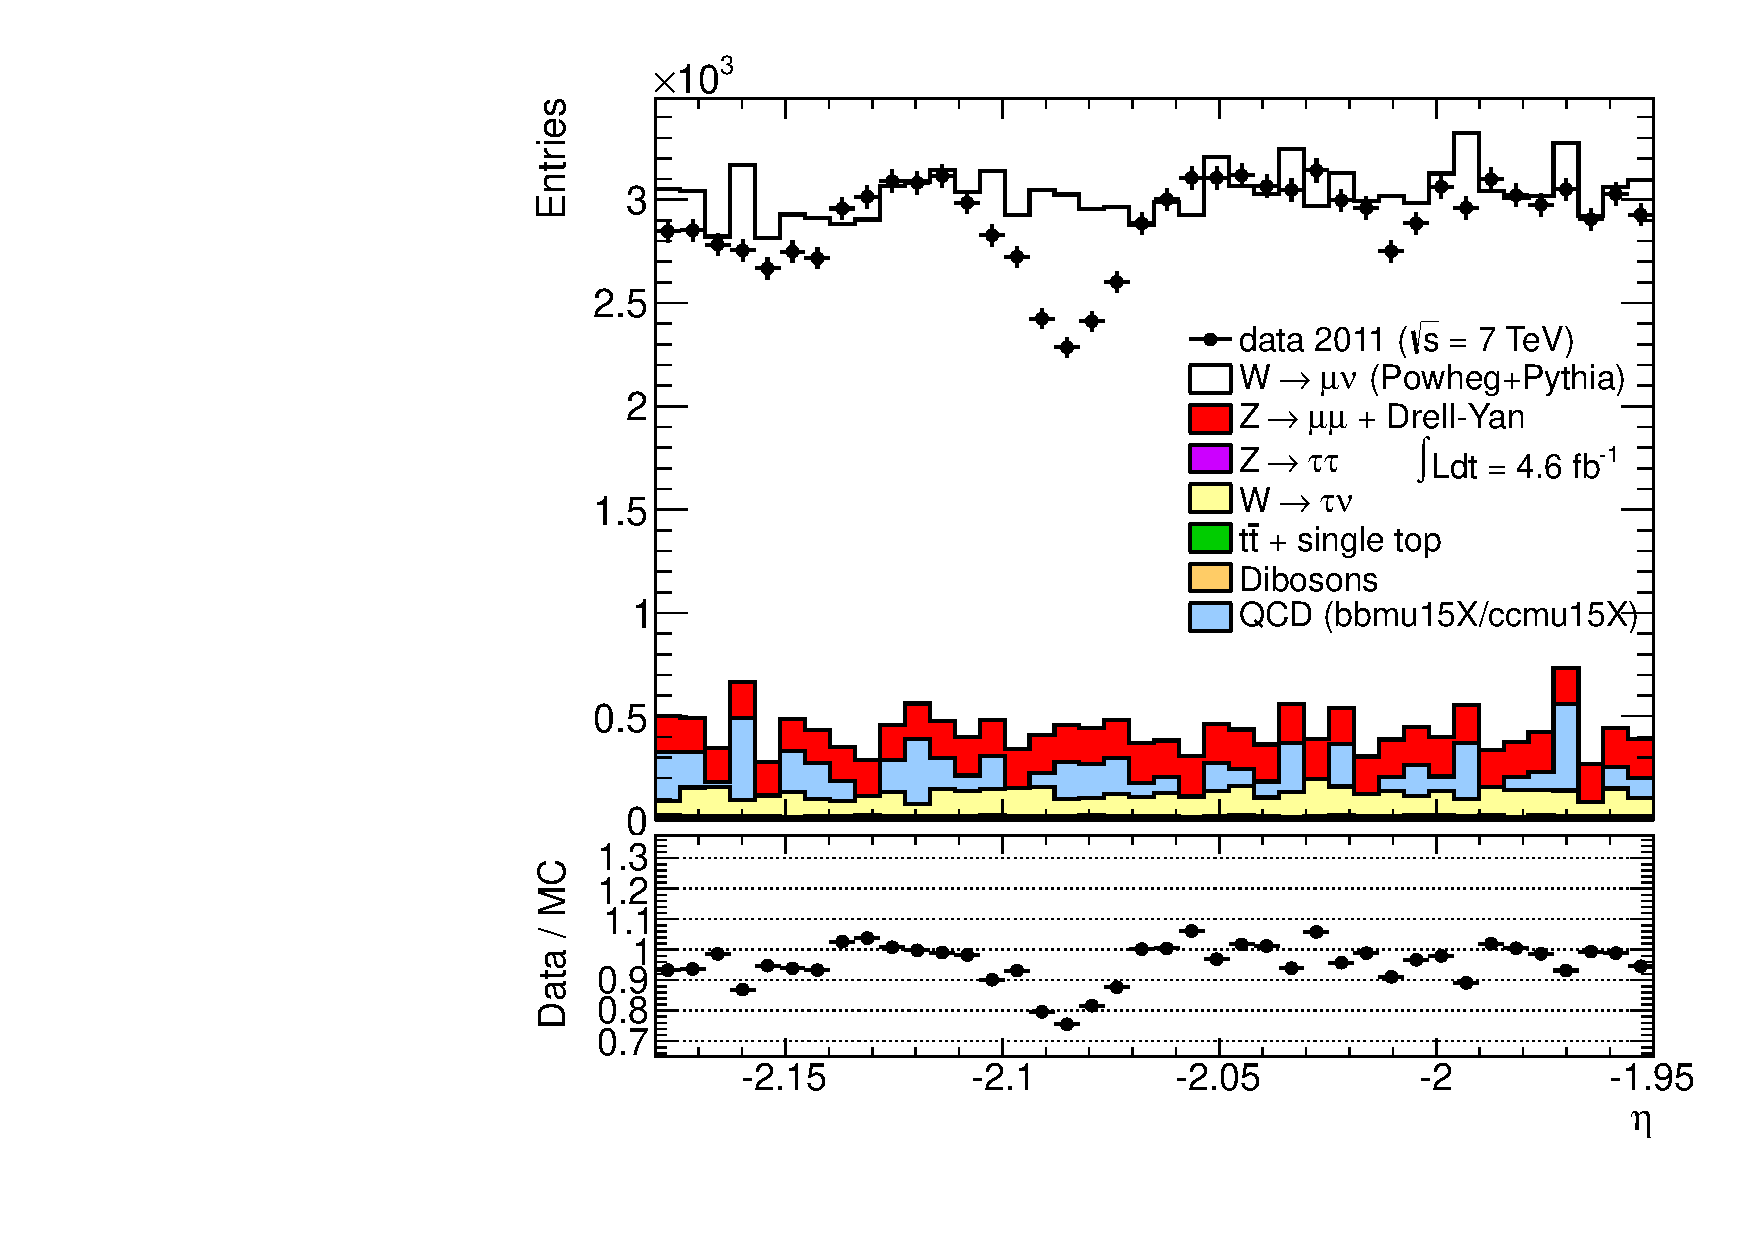
\includegraphics[width=0.66\textwidth]{dates/20130306/figures/etaphi/Wpt2535_10_C_stack_l_eta_NEG} \\
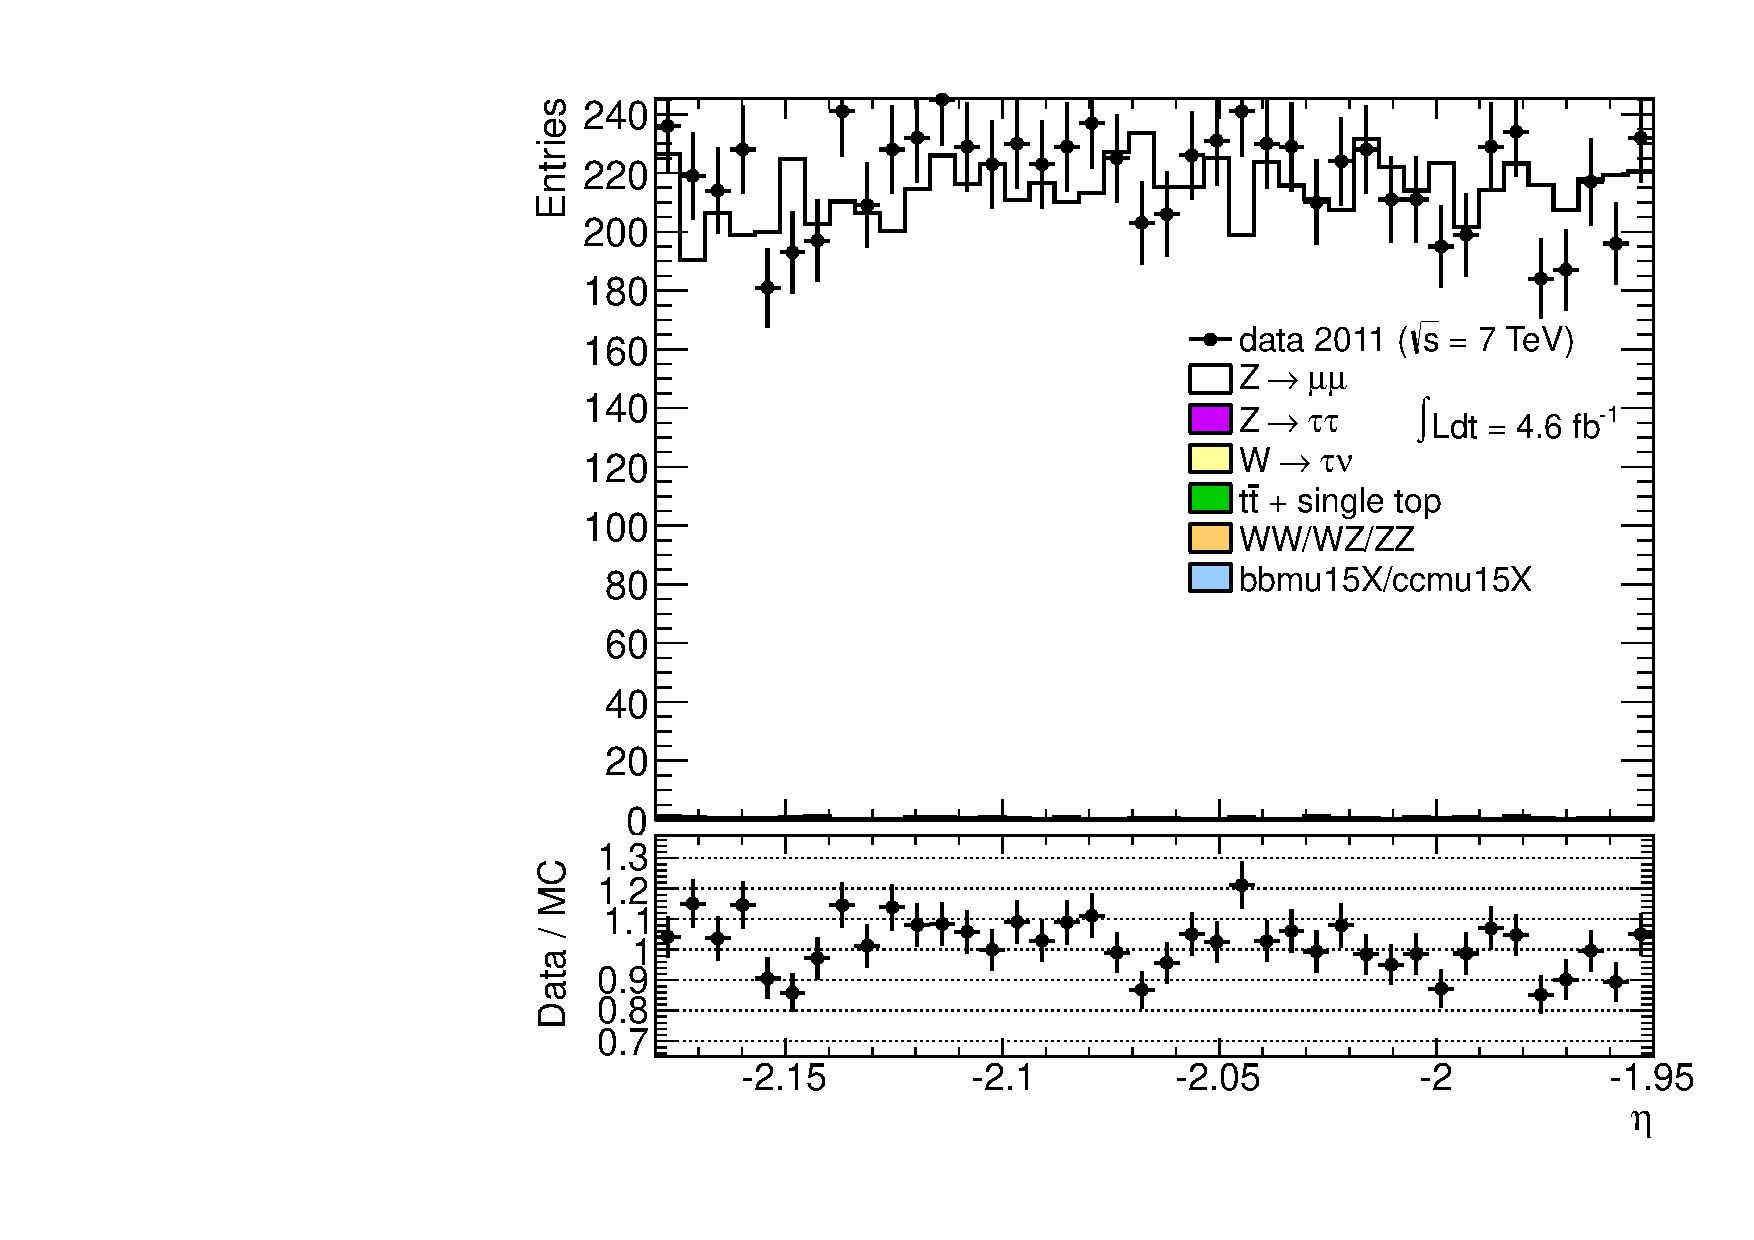
\includegraphics[width=0.66\textwidth]{dates/20130306/figures/etaphi/Zpt2535_10_C_stack_lN_eta_ALL.pdf}

\column{.5\textwidth}
A-side $\mu^{-}$ (top: W; bottom: Z)
\centering
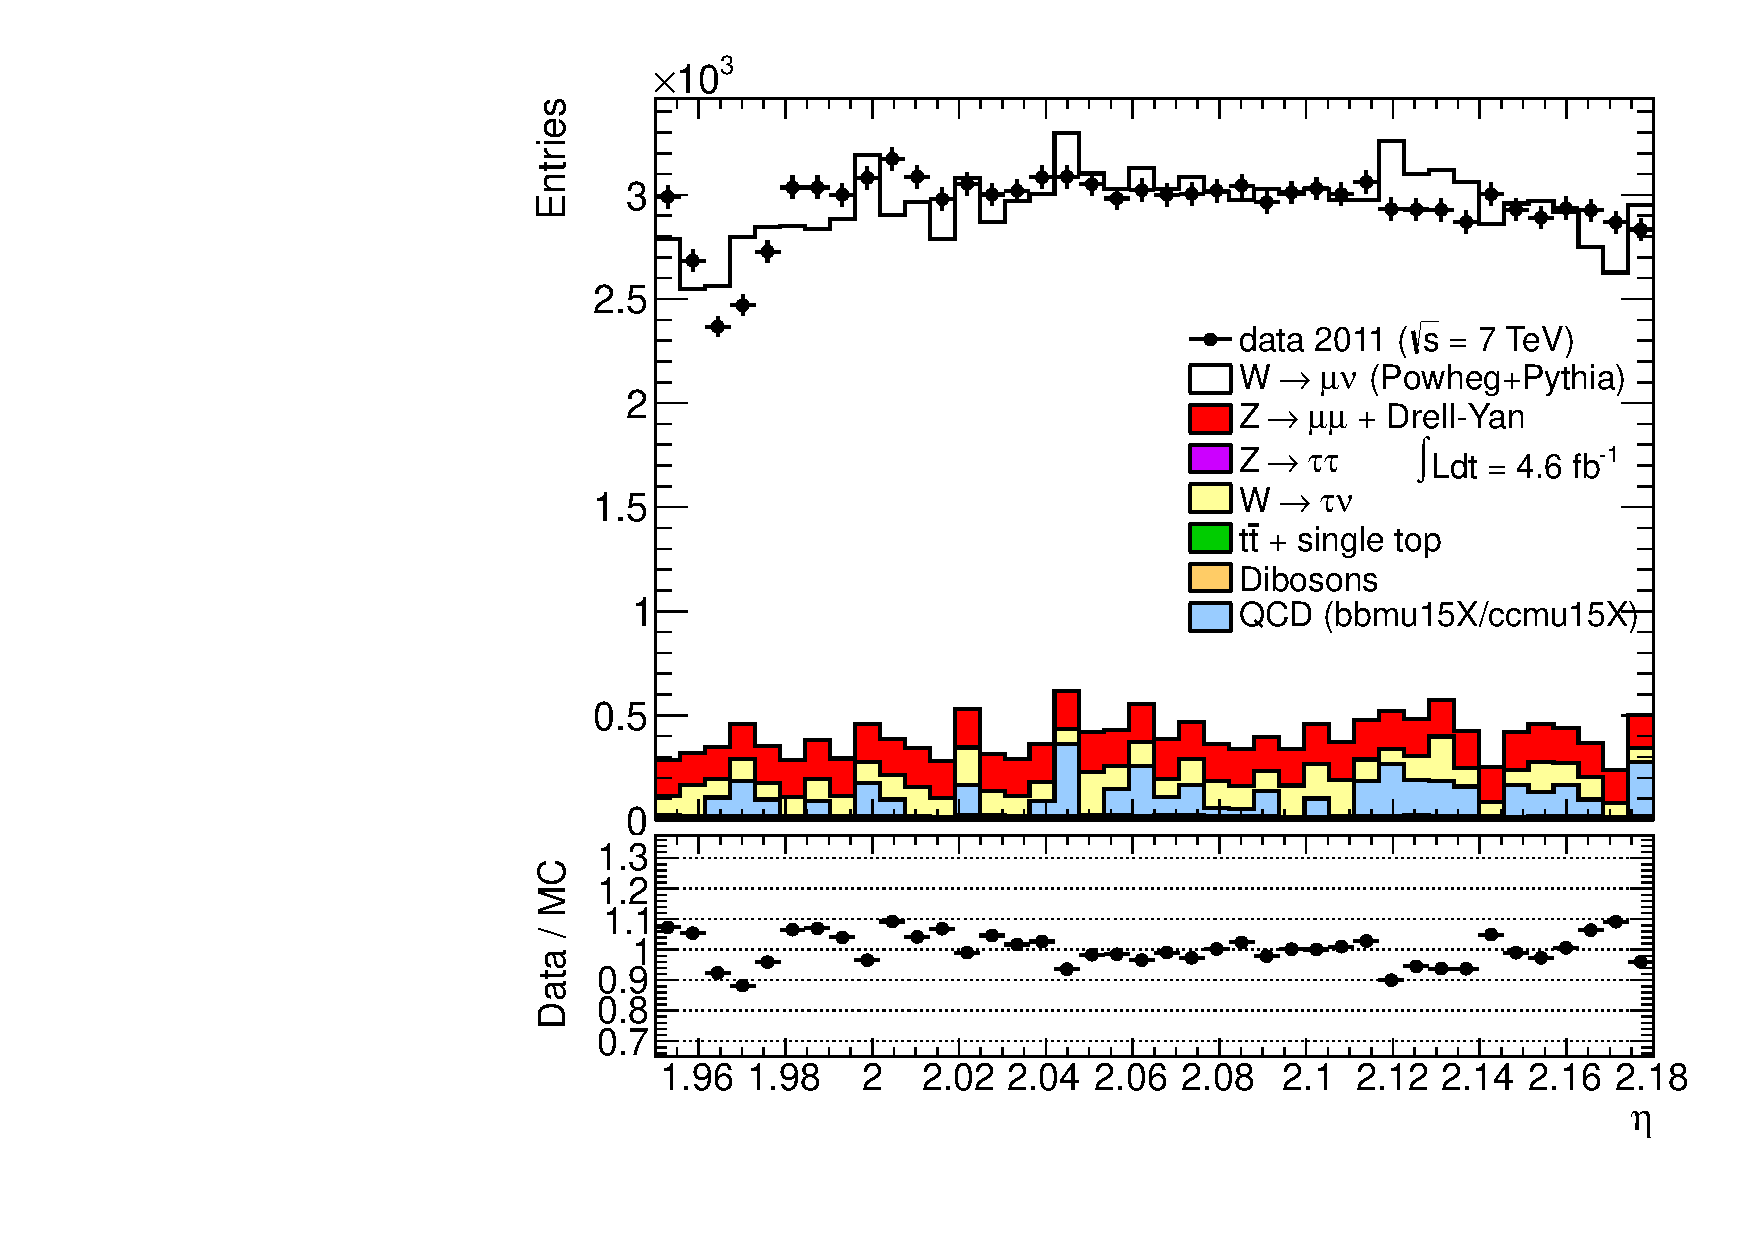
\includegraphics[width=0.66\textwidth]{dates/20130306/figures/etaphi/Wpt2535_10_A_stack_l_eta_NEG} \\
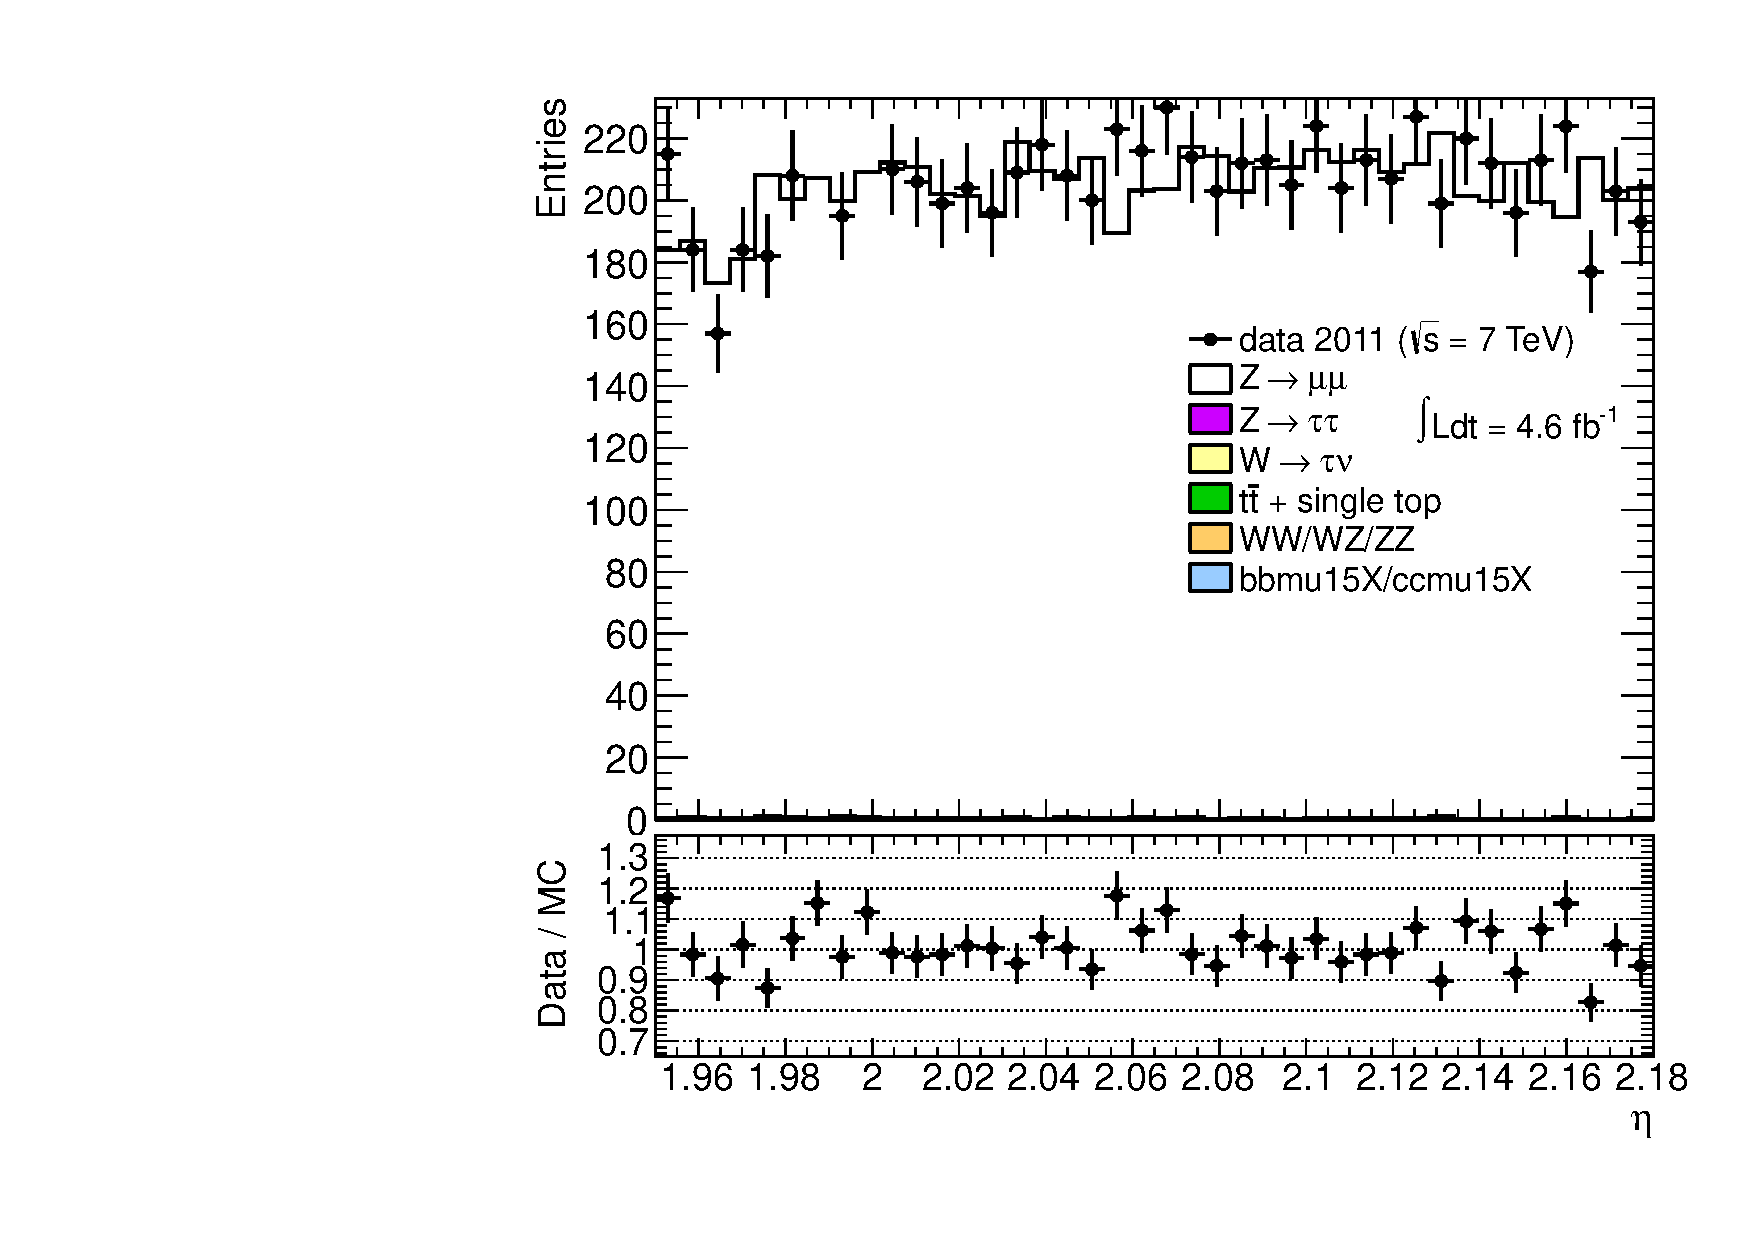
\includegraphics[width=0.66\textwidth]{dates/20130306/figures/etaphi/Zpt2535_10_A_stack_lN_eta_ALL.pdf} 

\cole
}


\only<11>{
Recall that in the A/C slide, there was a hint that $Z+jets$ may exhibit the dip. \\
(njets cut was added to break the phi correlation between the two Z muons).
Let's look at $\eta$ and $\phi$ with $njets>=1$ for both W and Z muons.
}

\only<12> {
\colb[T]

\column{.5\textwidth}
C-side $\mu^{-}$ (top: W; bottom: Z)
\centering
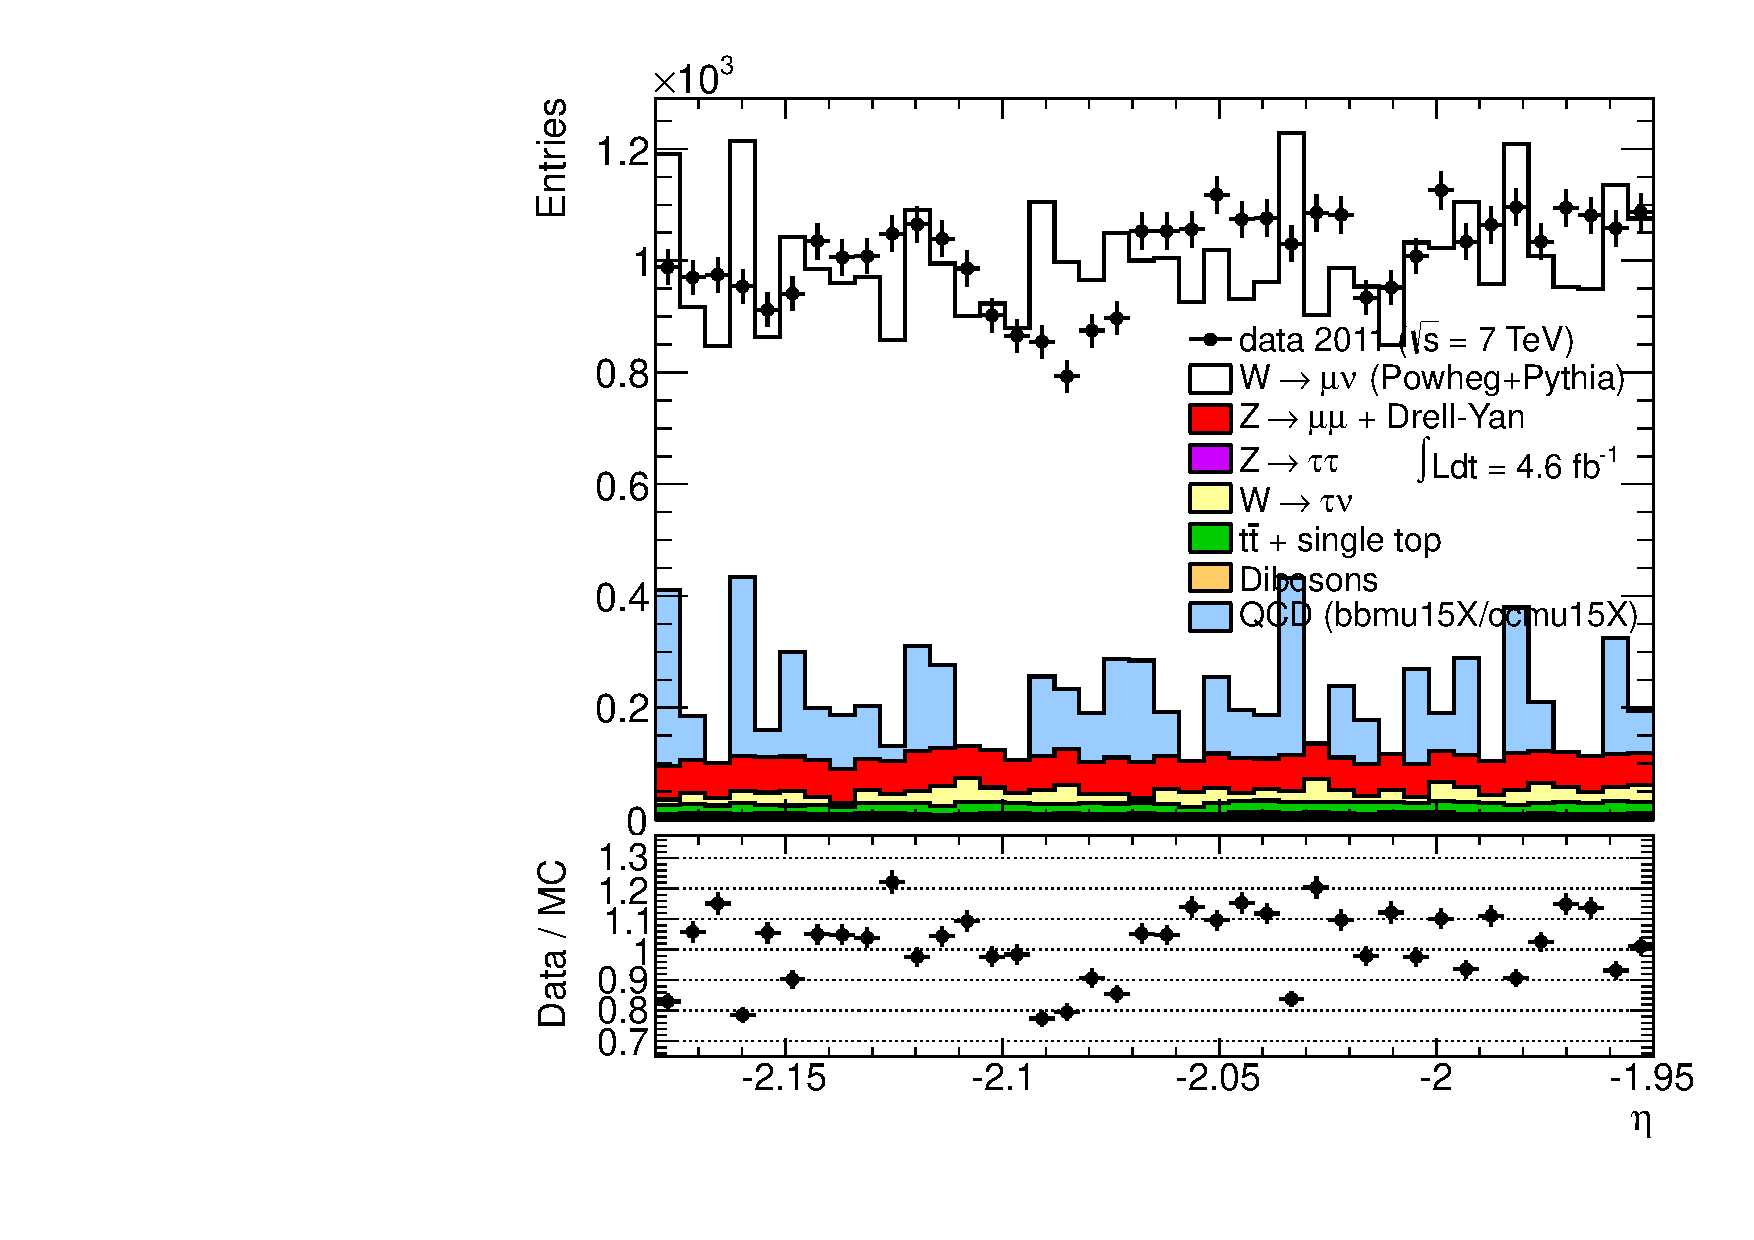
\includegraphics[width=0.66\textwidth]{dates/20130306/figures/etaphi/Wnjets_10_C_stack_l_eta_NEG} \\
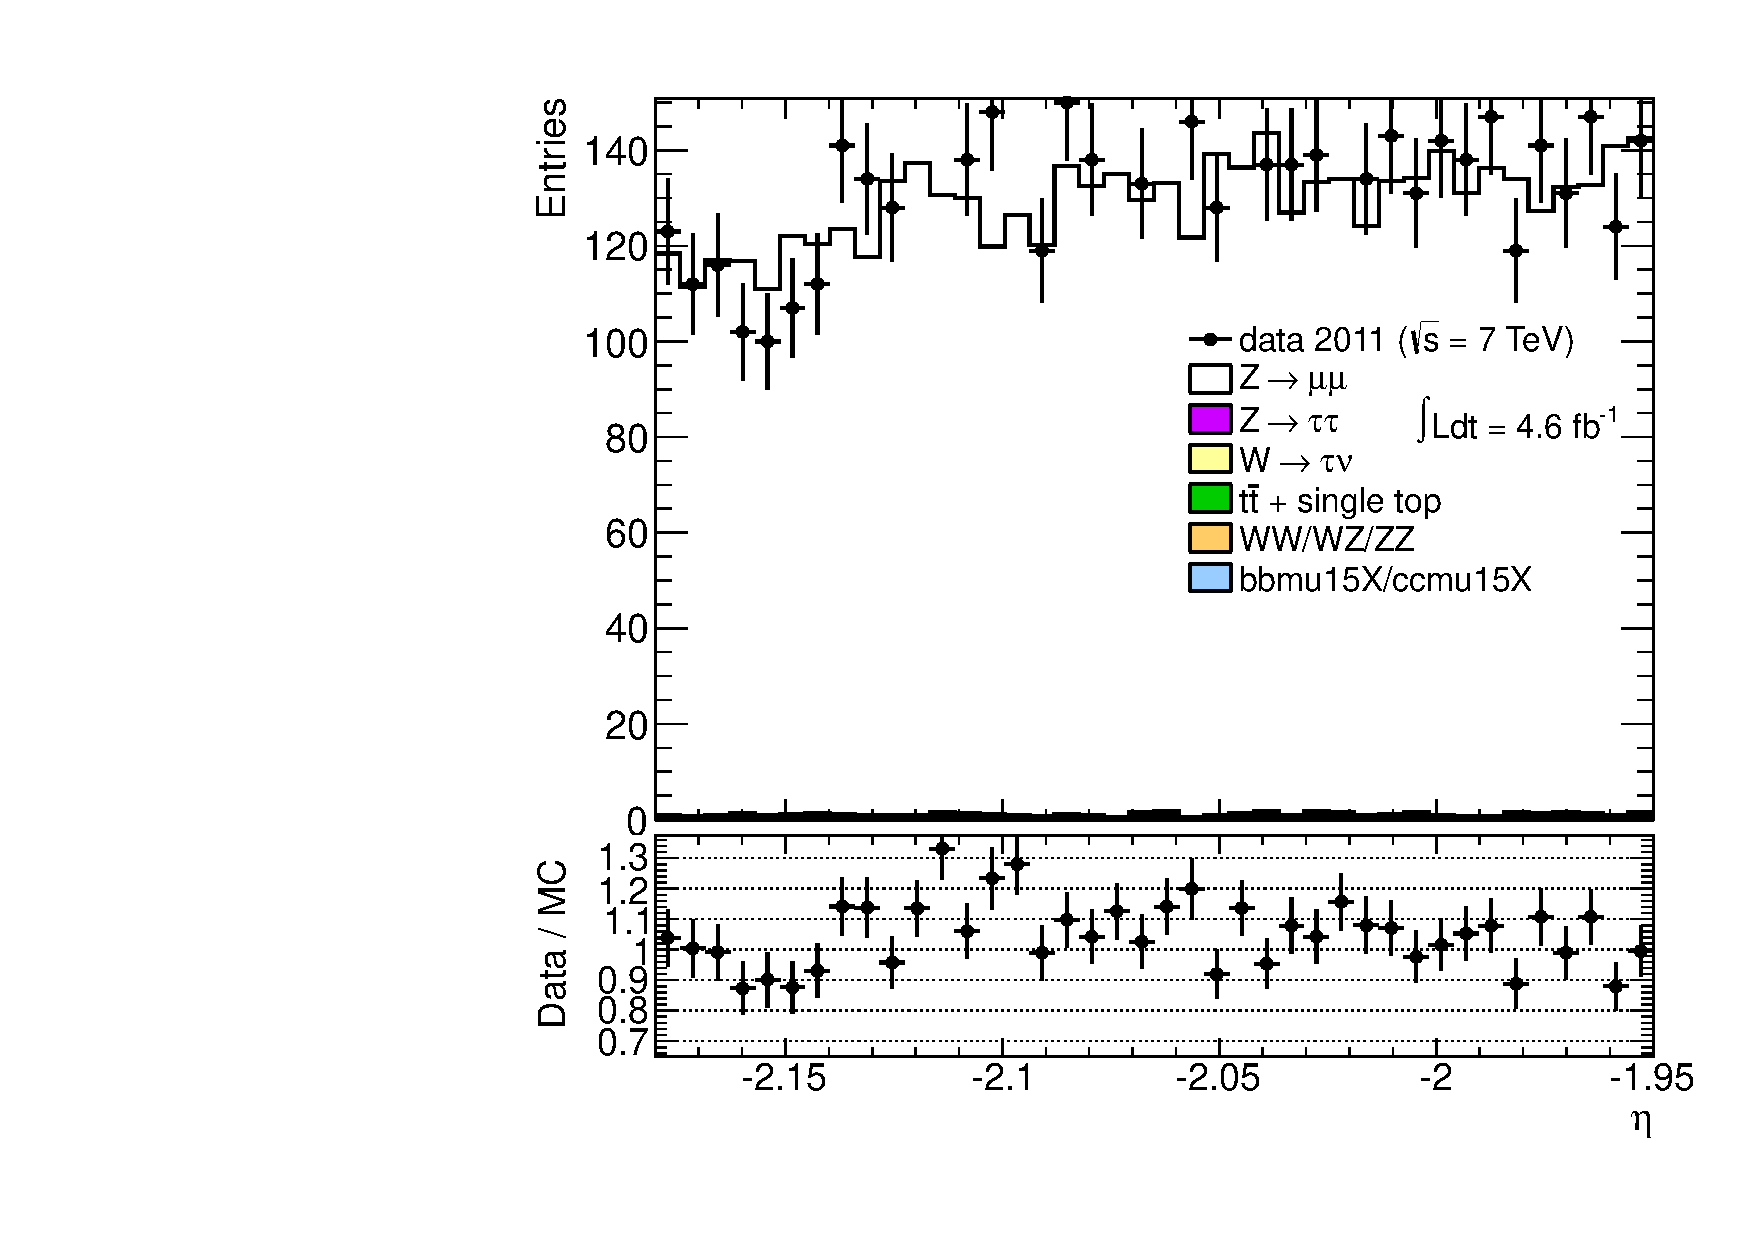
\includegraphics[width=0.66\textwidth]{dates/20130306/figures/etaphi/Znjets_10_C_stack_lN_eta_ALL.pdf}

\column{.5\textwidth}
A-side $\mu^{-}$ (top: W; bottom: Z)
\centering
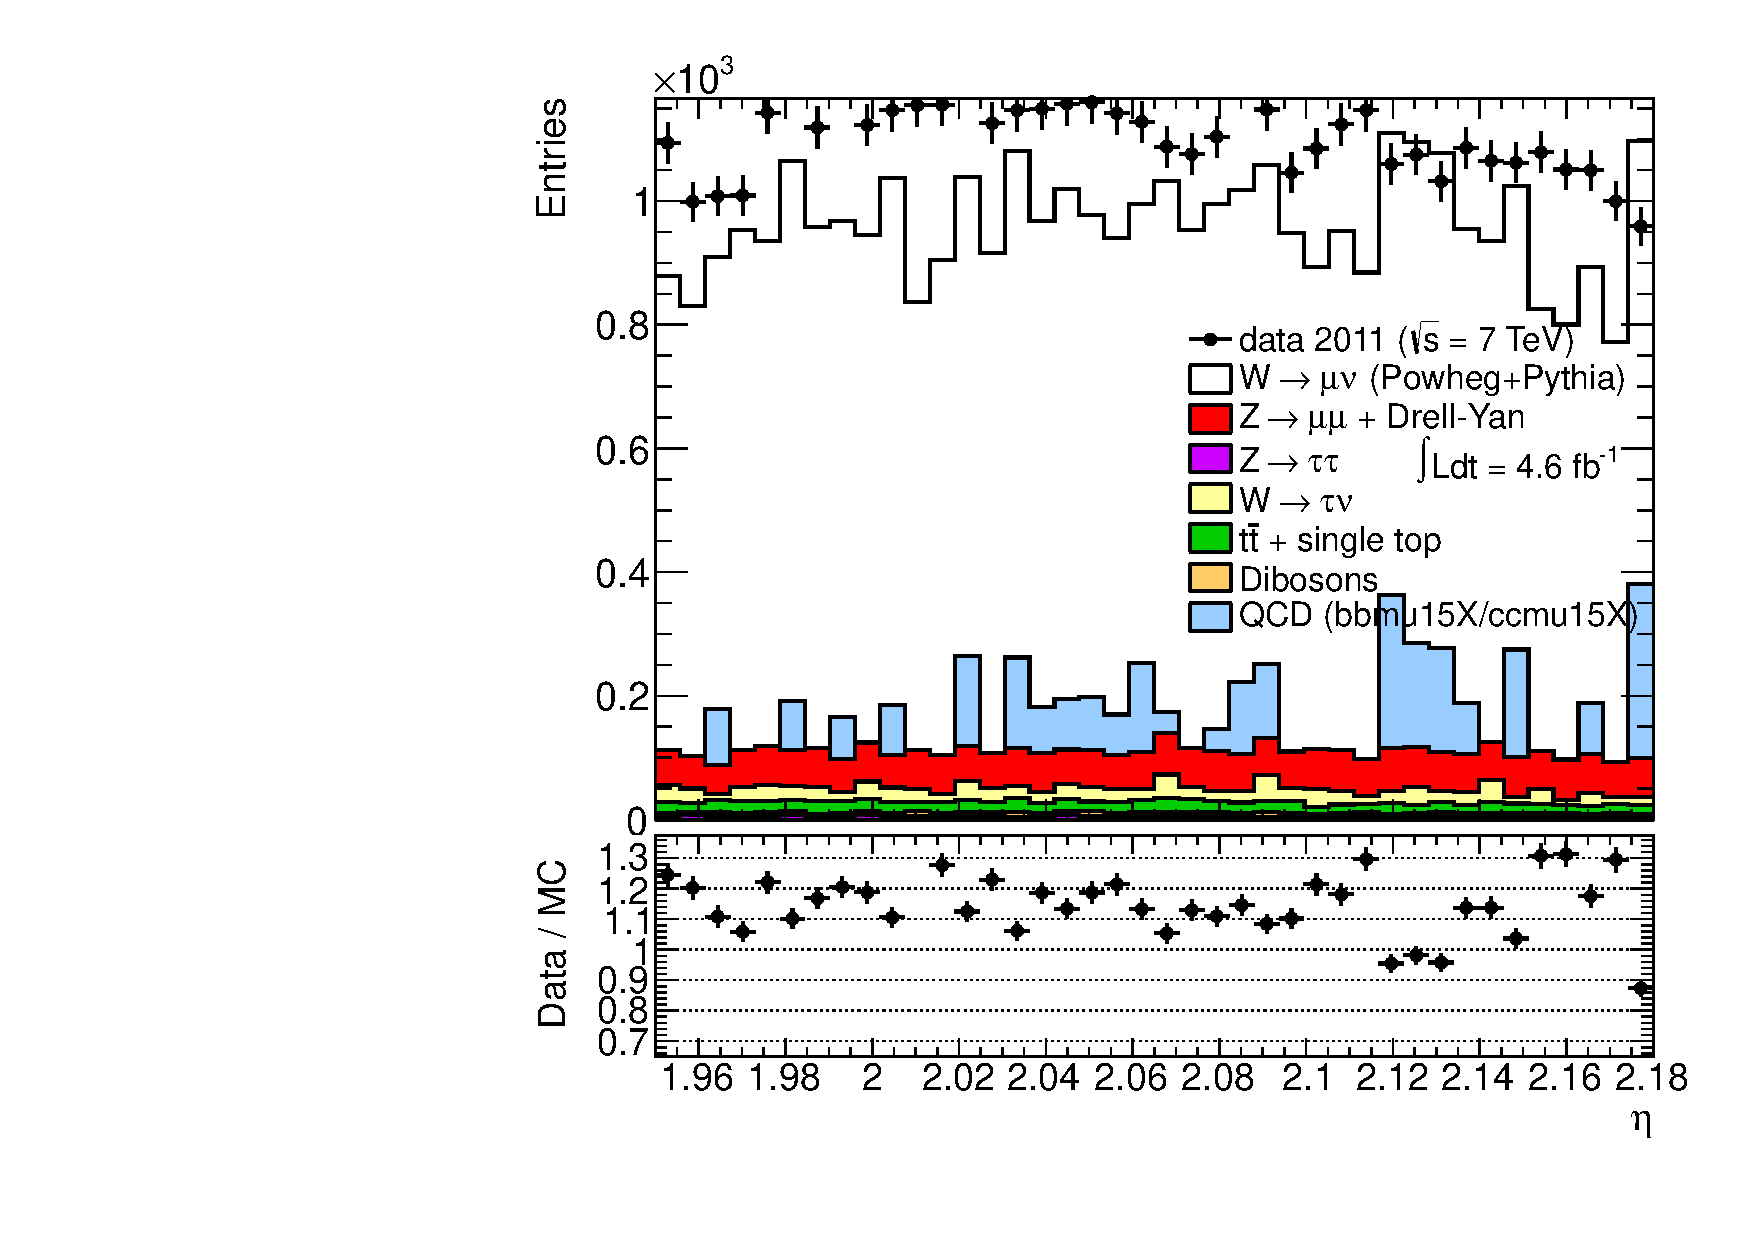
\includegraphics[width=0.66\textwidth]{dates/20130306/figures/etaphi/Wnjets_10_A_stack_l_eta_NEG} \\
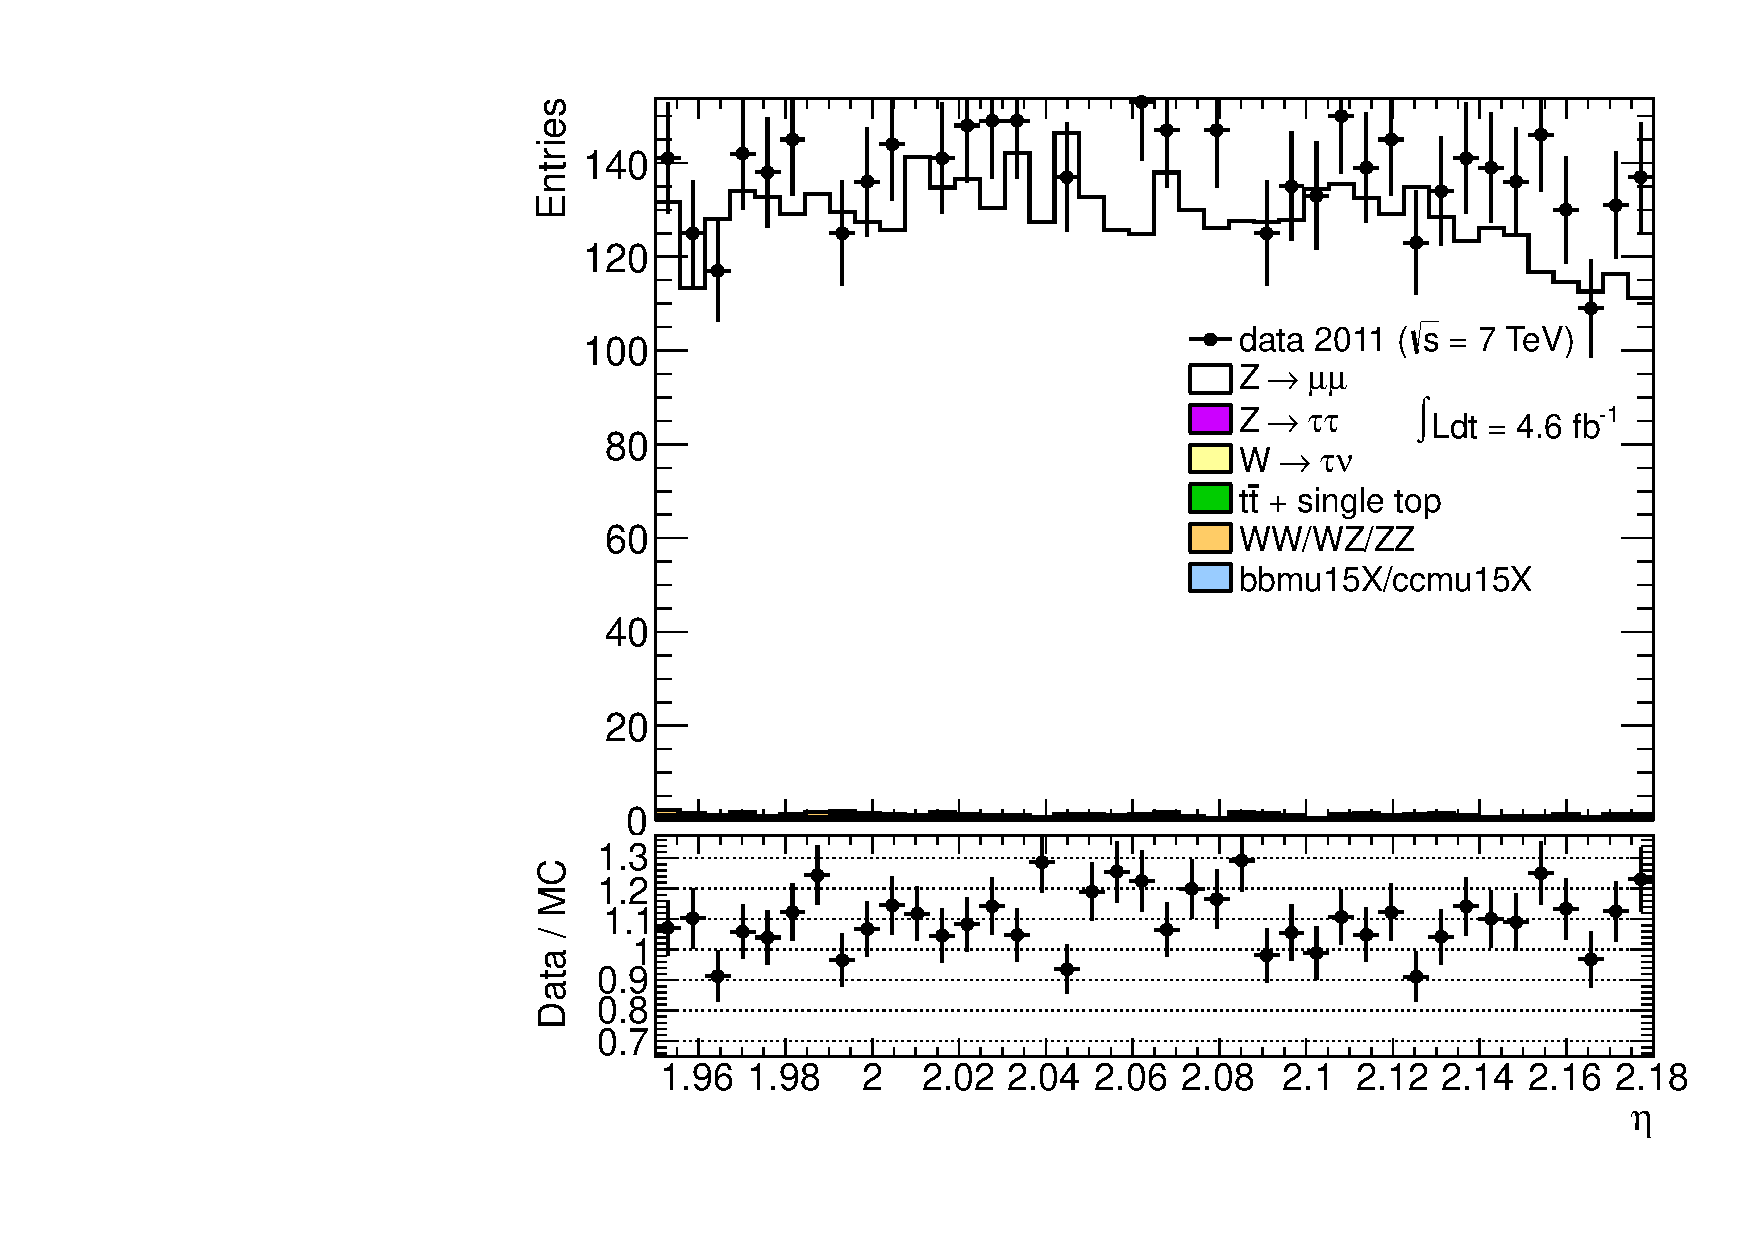
\includegraphics[width=0.66\textwidth]{dates/20130306/figures/etaphi/Znjets_10_A_stack_lN_eta_ALL.pdf} 

\cole
}


\only<13>{
Another way to break the Z muon correlations: \\
Force the other (tag) muon to be in the \red{barrel}.
}

\only<14> {
\colb[T]

\column{.5\textwidth}
C-side $\mu^{-}$ (top: W; bottom: Z)
\centering
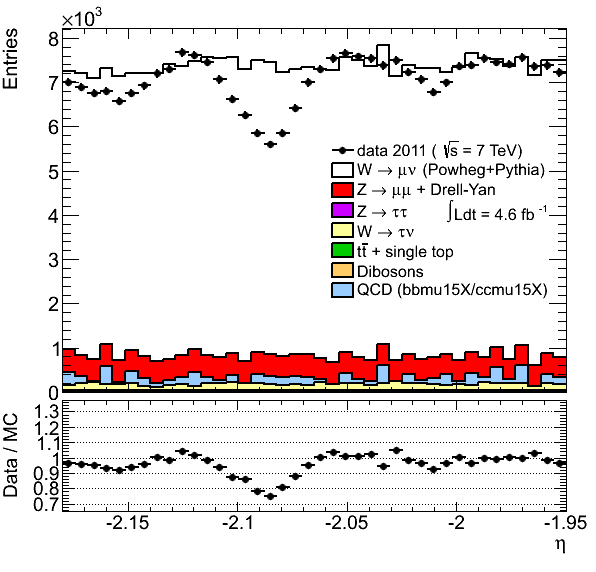
\includegraphics[width=0.66\textwidth]{dates/20130306/figures/etaphi/W_10_C_stack_l_eta_NEG} \\
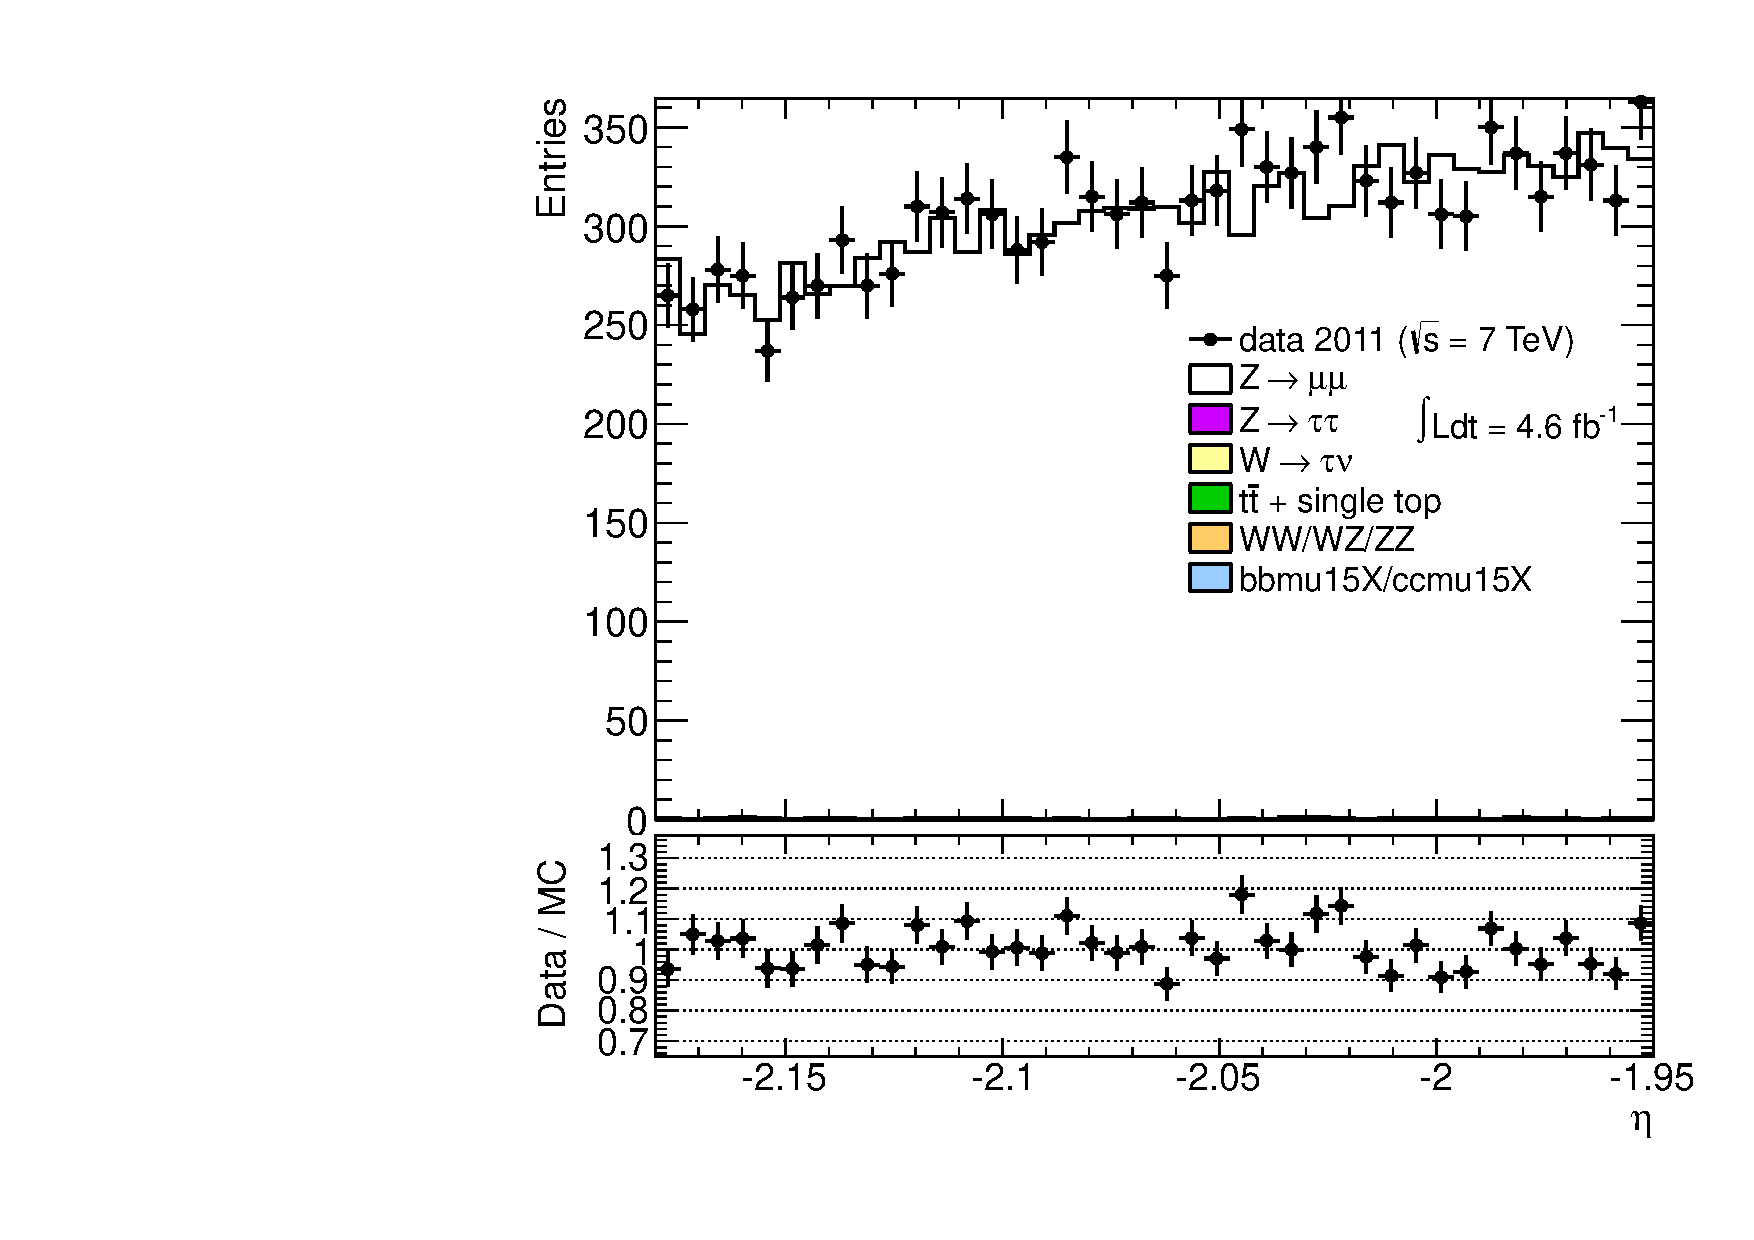
\includegraphics[width=0.66\textwidth]{dates/20130306/figures/etaphi/ZlObarrel_10_C_stack_lN_eta_ALL.pdf}

\column{.5\textwidth}
A-side $\mu^{-}$ (top: W; bottom: Z)
\centering
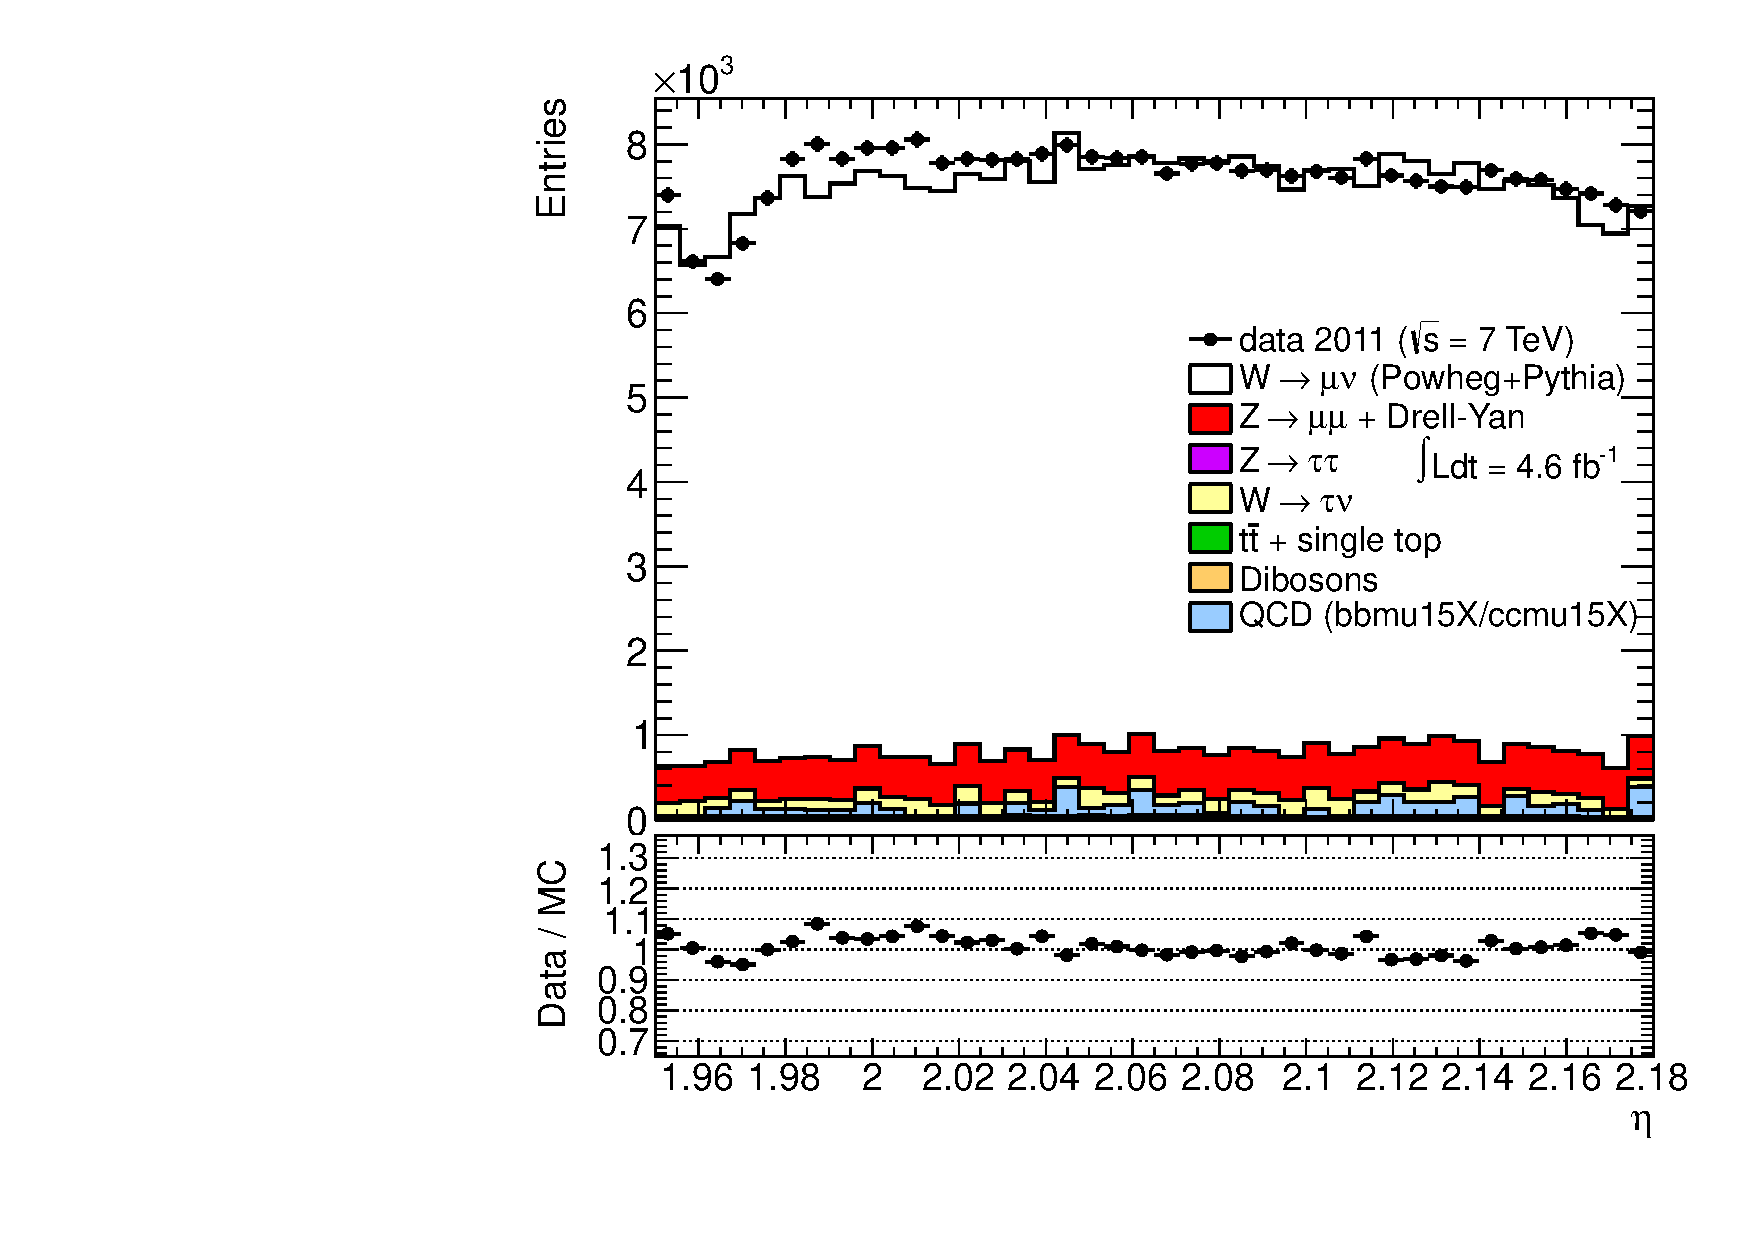
\includegraphics[width=0.66\textwidth]{dates/20130306/figures/etaphi/W_10_A_stack_l_eta_NEG} \\
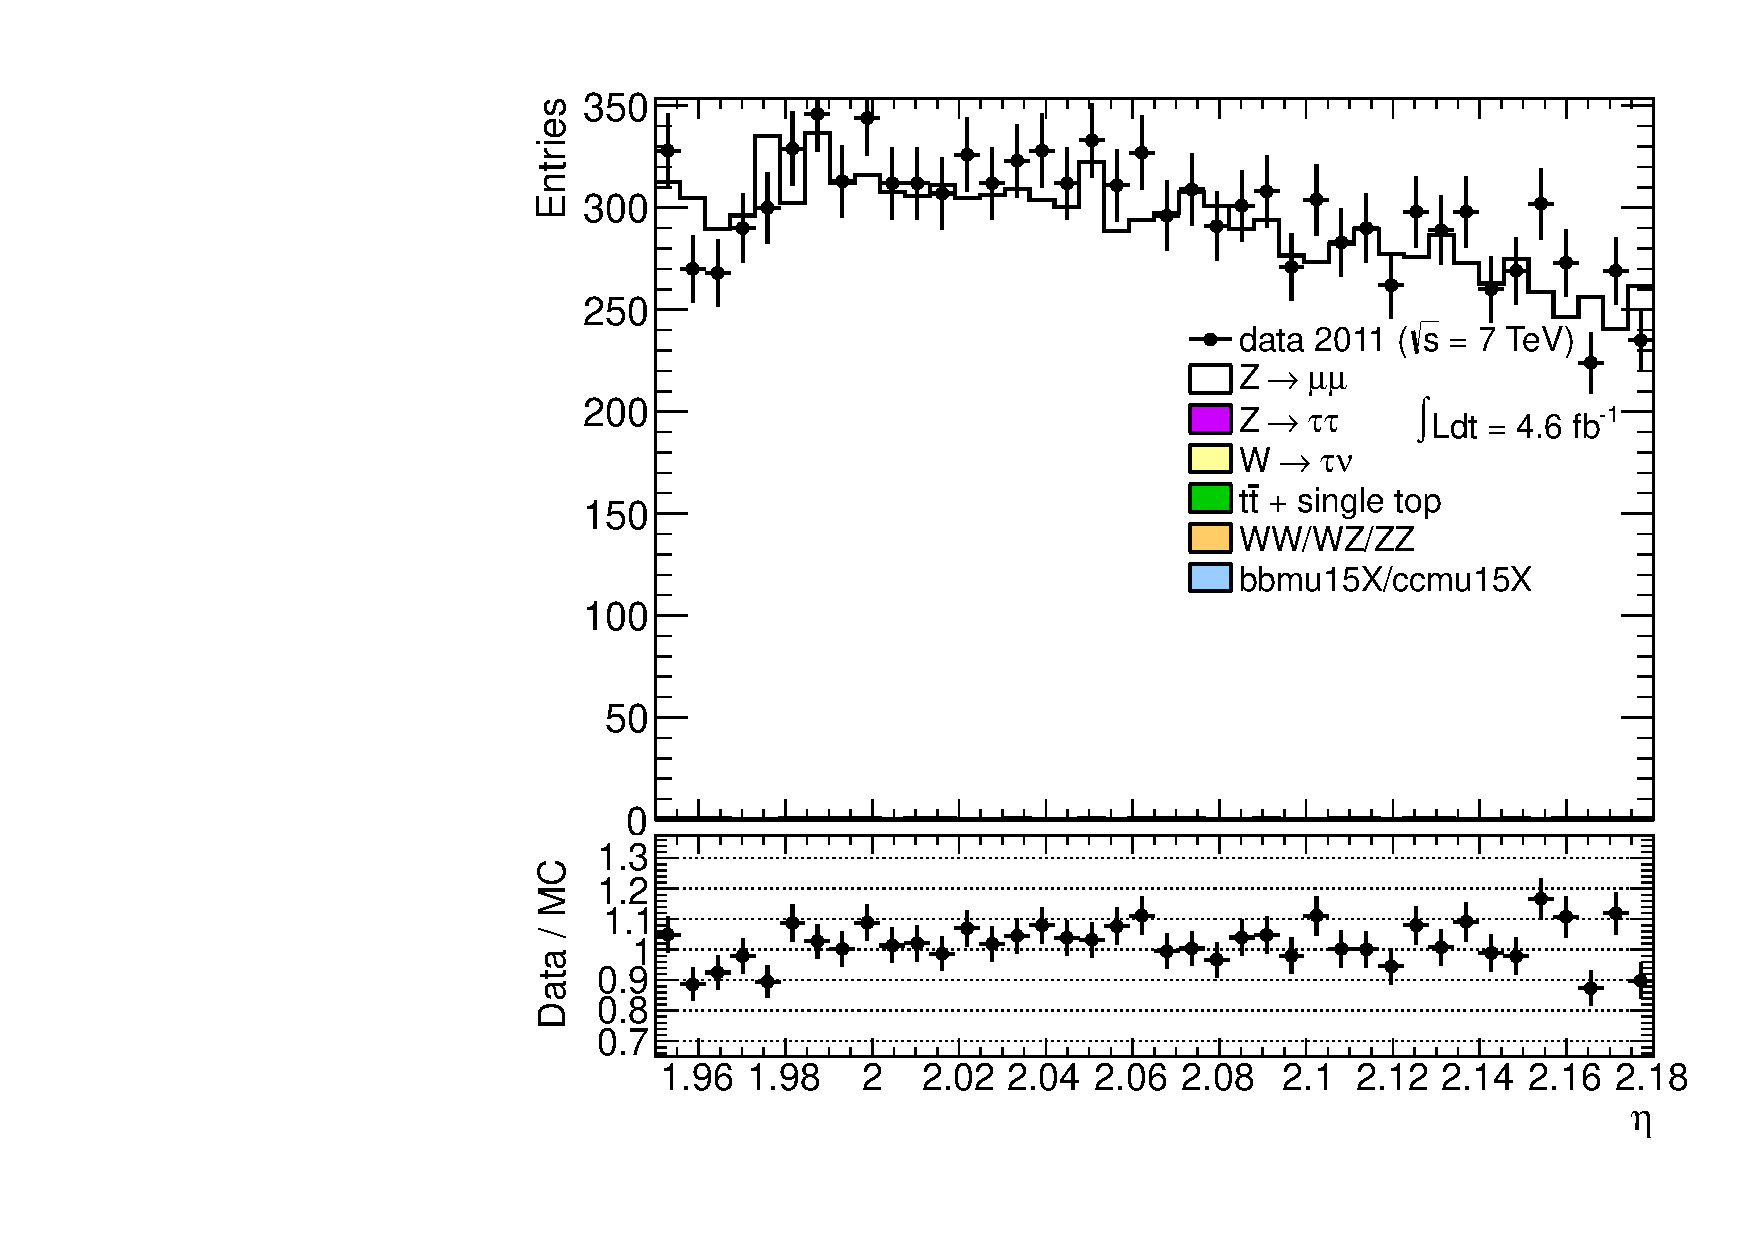
\includegraphics[width=0.66\textwidth]{dates/20130306/figures/etaphi/ZlObarrel_10_A_stack_lN_eta_ALL.pdf} 

\cole
}


\only<15>{
For completeness, let's force the other (tag) muon to be in the \red{endcap}.
}

\only<16> {
\colb[T]

\column{.5\textwidth}
C-side $\mu^{-}$ (top: W; bottom: Z)
\centering
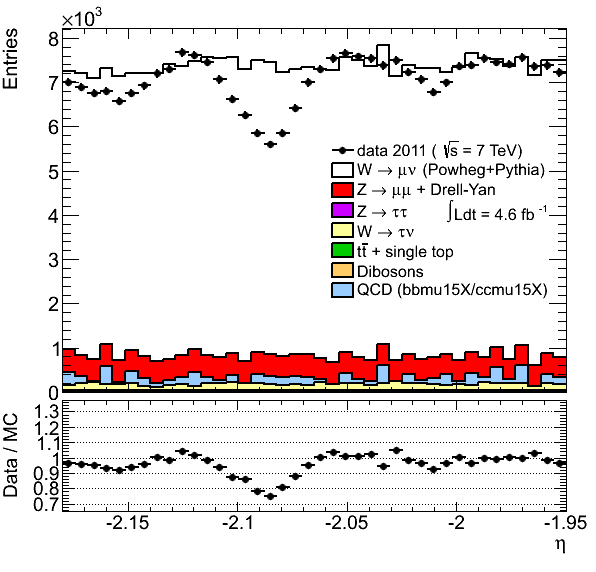
\includegraphics[width=0.66\textwidth]{dates/20130306/figures/etaphi/W_10_C_stack_l_eta_NEG} \\
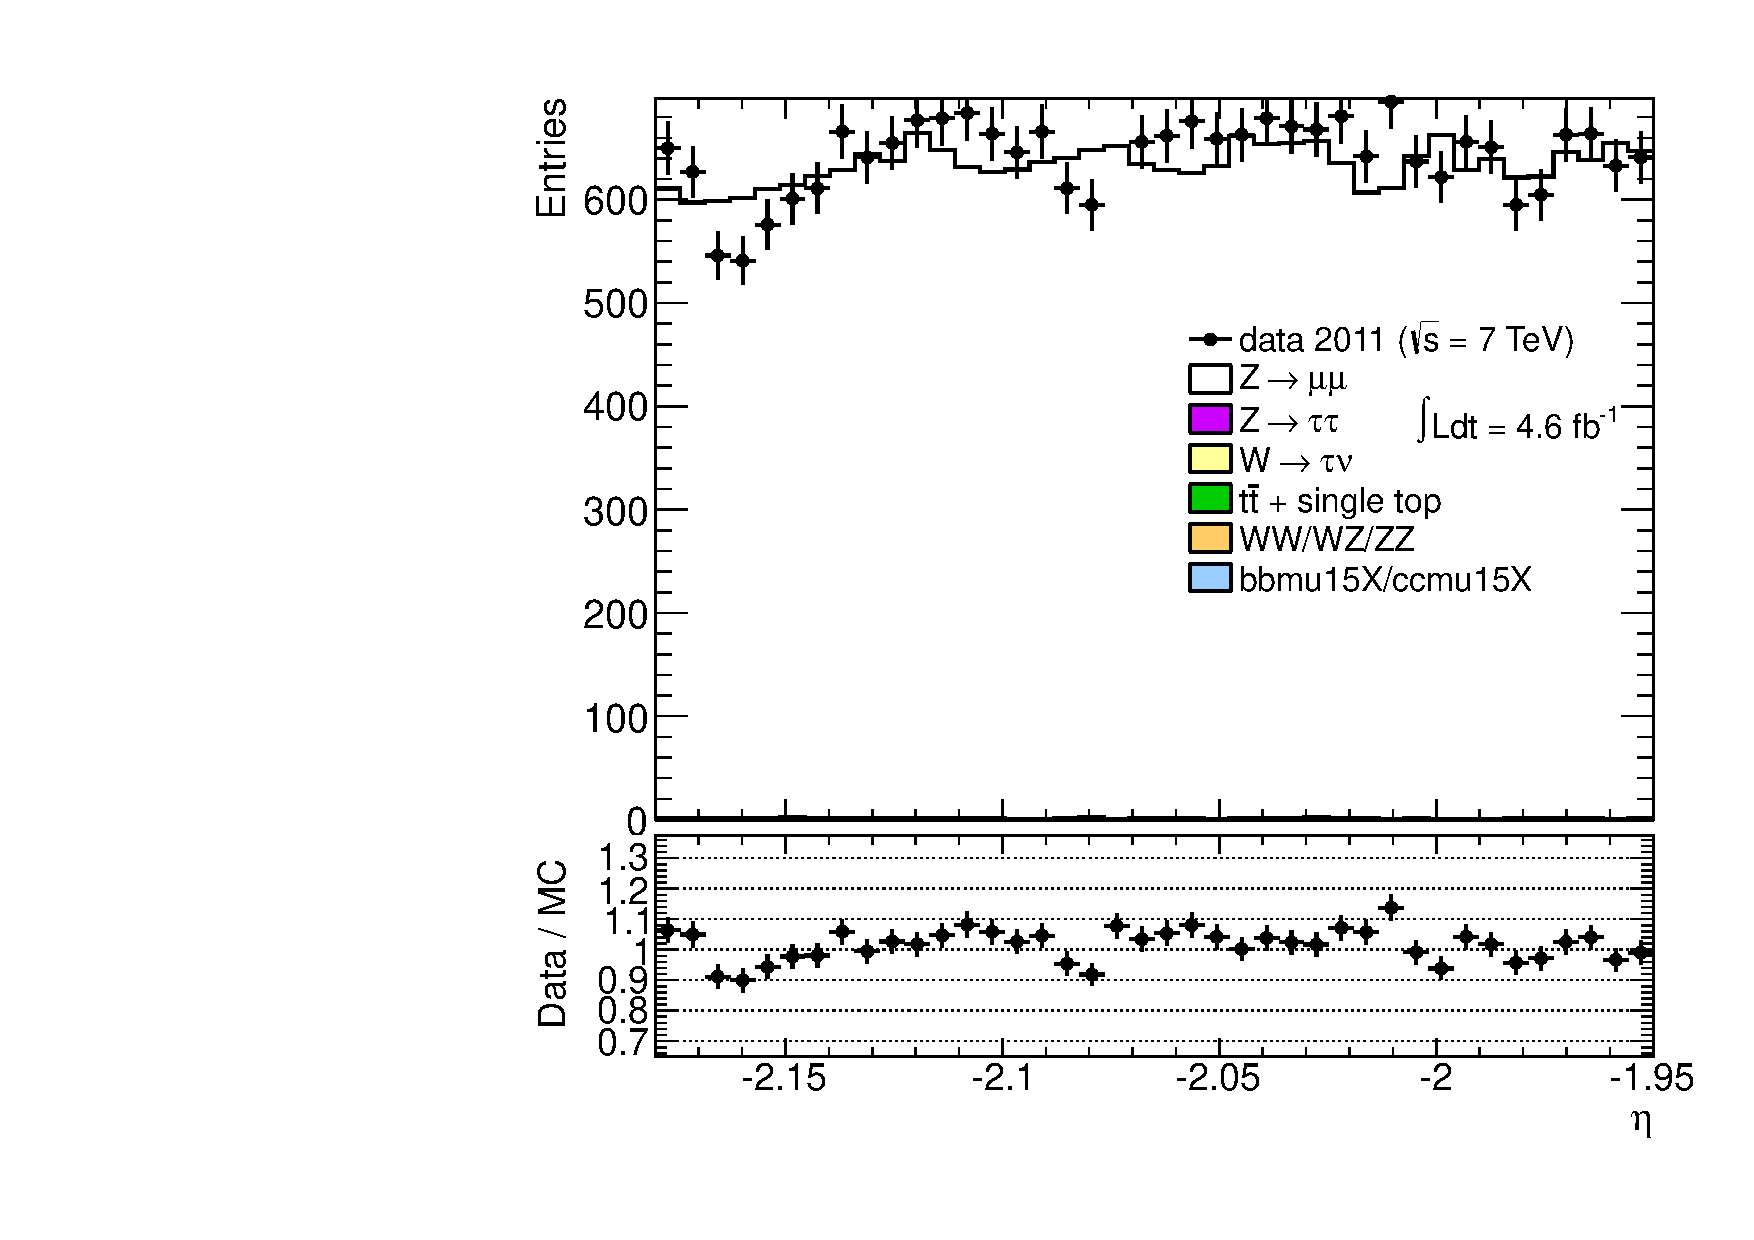
\includegraphics[width=0.66\textwidth]{dates/20130306/figures/etaphi/ZlOendcap_10_C_stack_lN_eta_ALL.pdf}

\column{.5\textwidth}
A-side $\mu^{-}$ (top: W; bottom: Z)
\centering
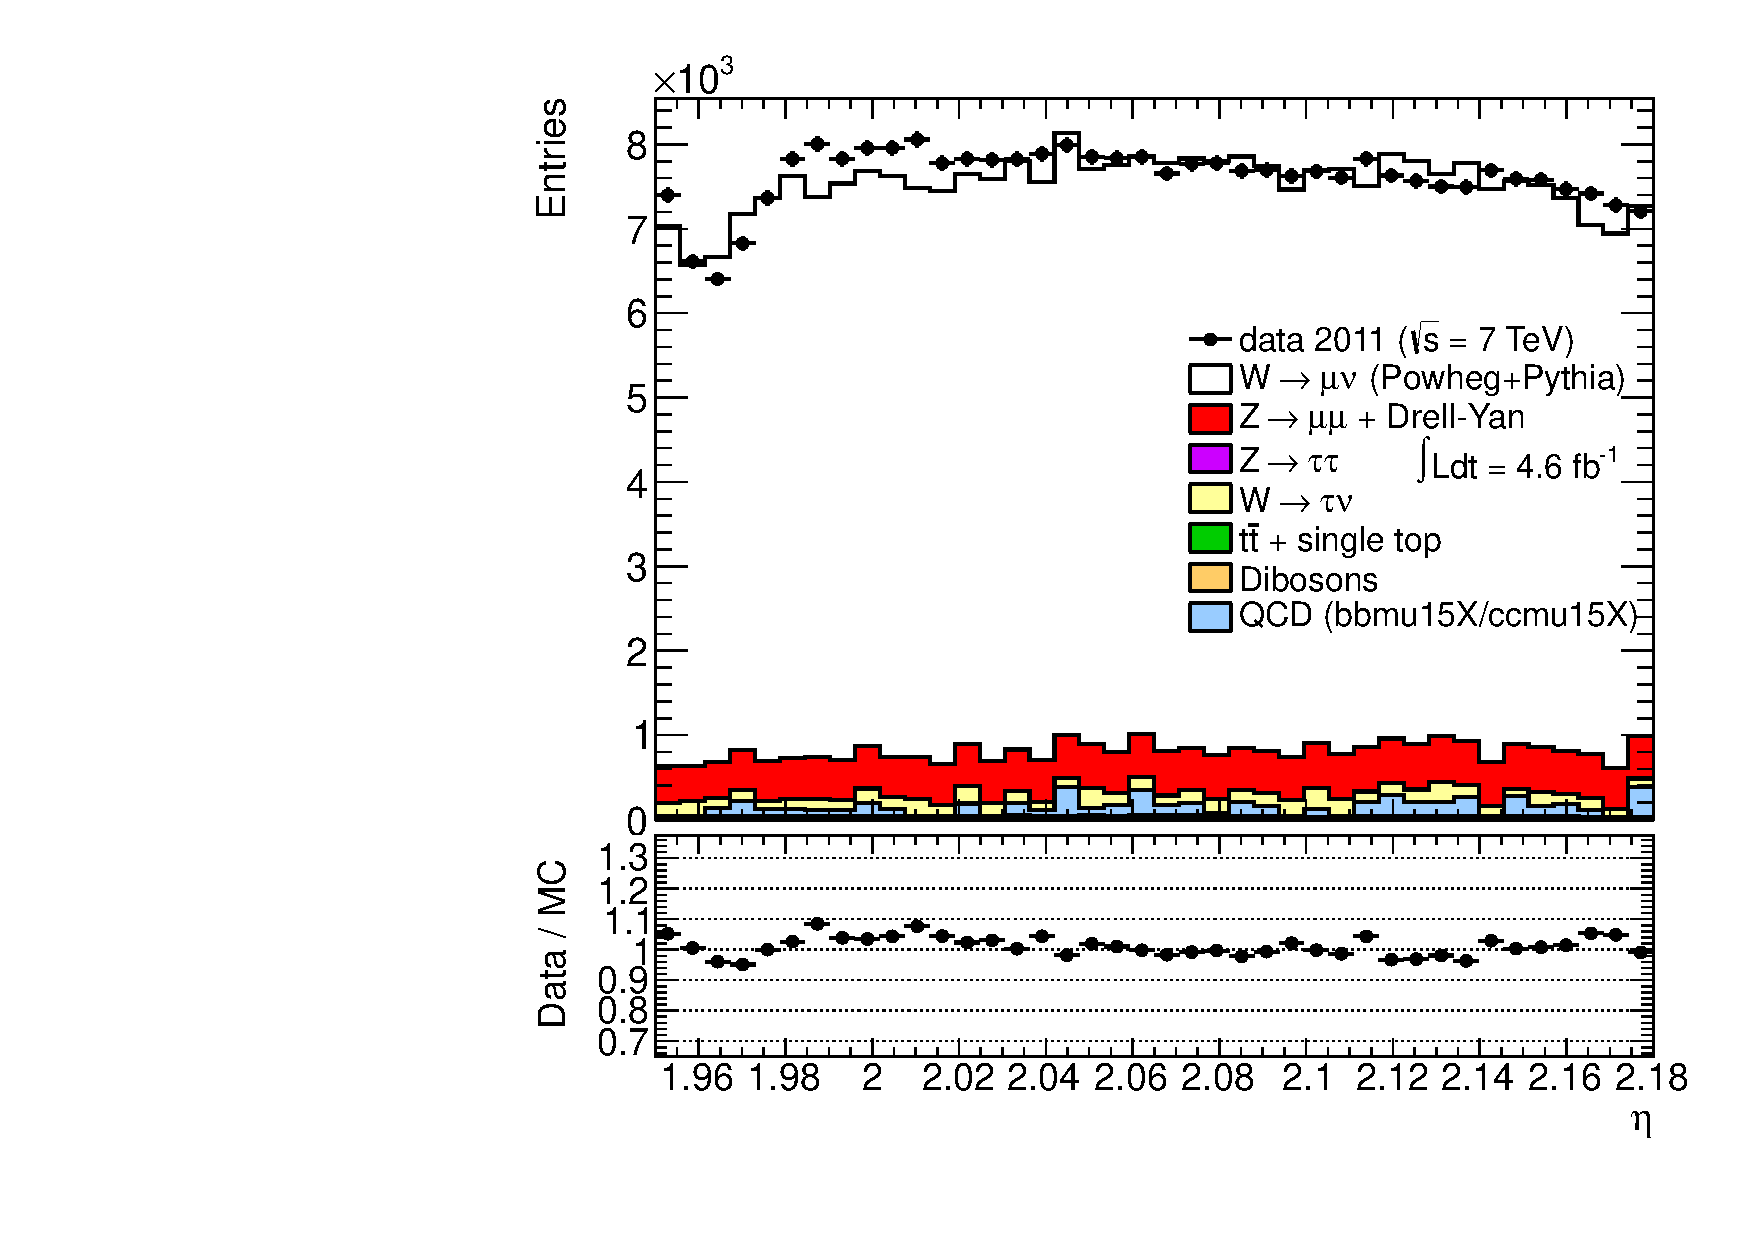
\includegraphics[width=0.66\textwidth]{dates/20130306/figures/etaphi/W_10_A_stack_l_eta_NEG} \\
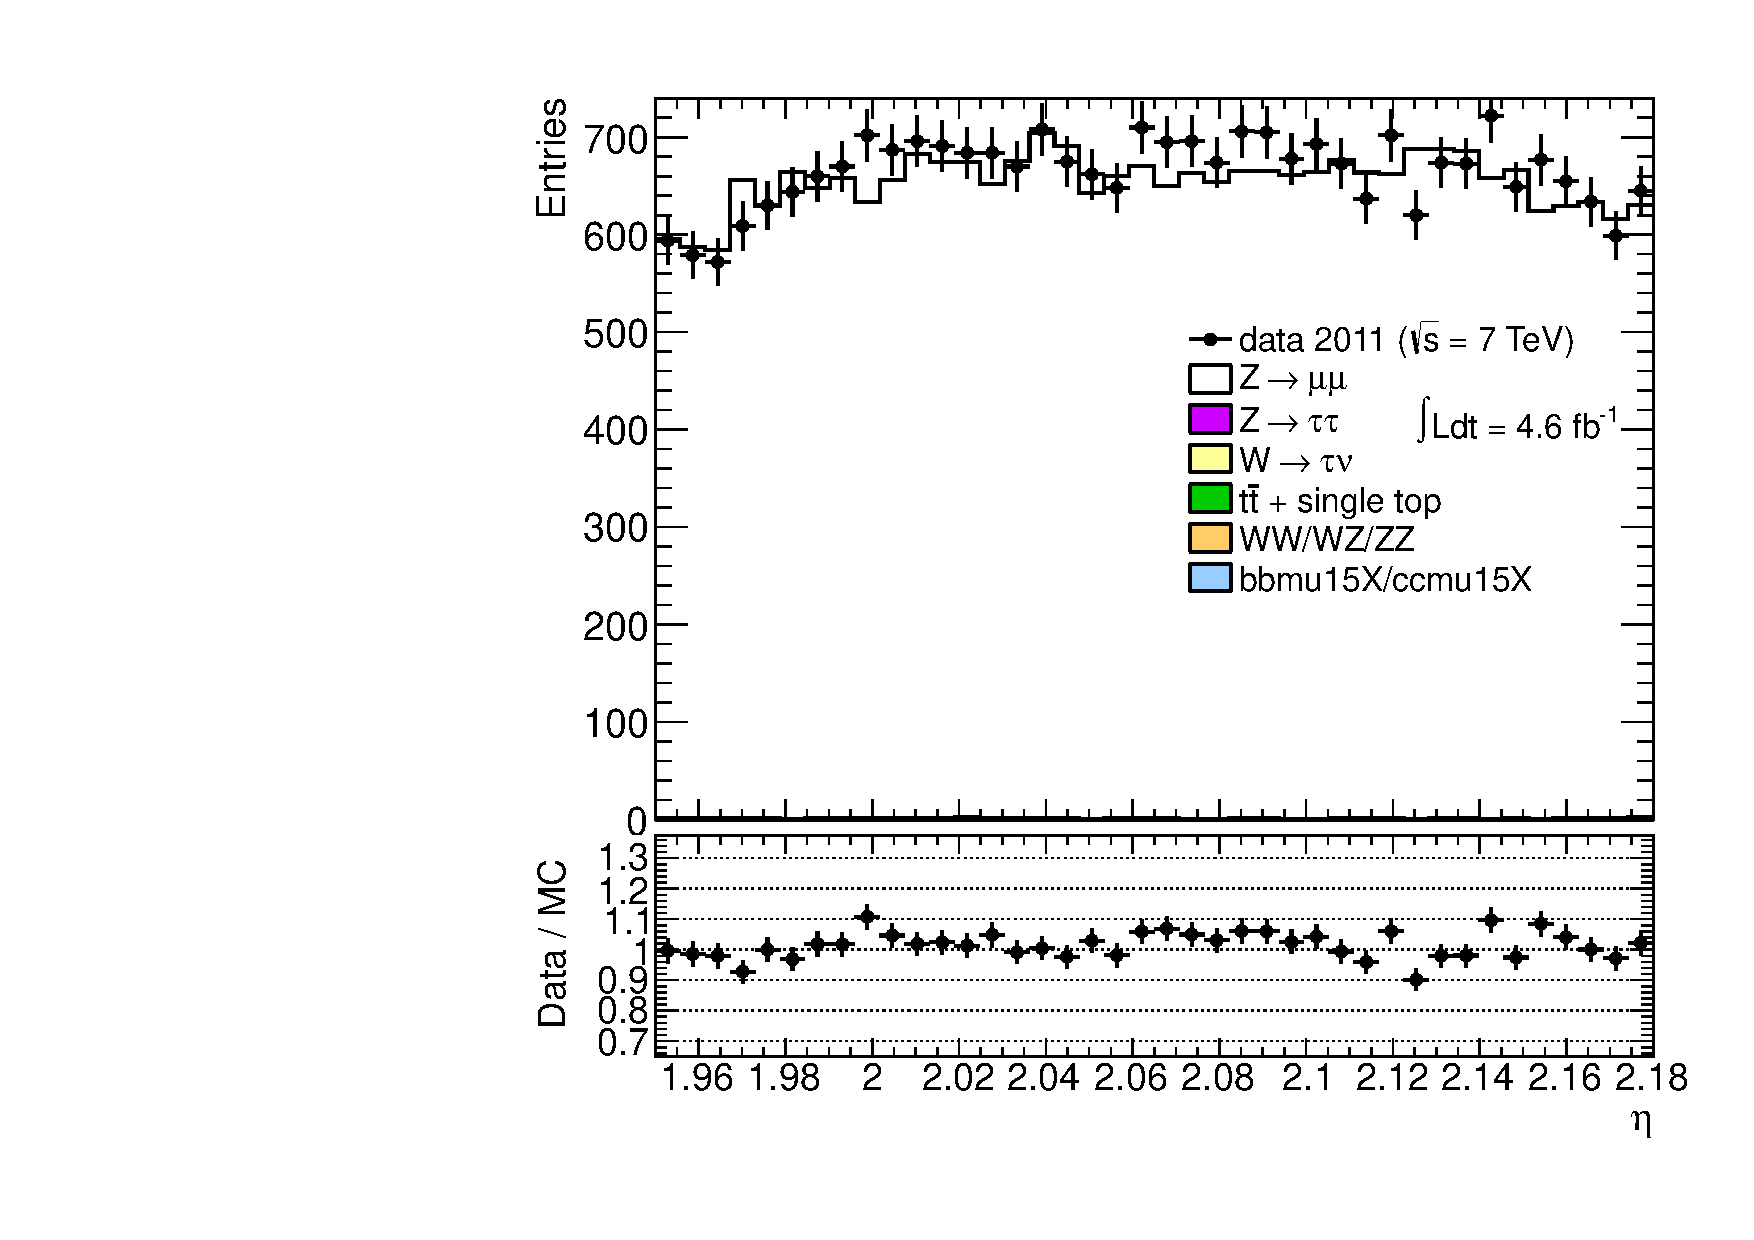
\includegraphics[width=0.66\textwidth]{dates/20130306/figures/etaphi/ZlOendcap_10_A_stack_lN_eta_ALL.pdf} 

\cole
}


\only<17>{
What if we have very poorly reconstructed muons around the dip? \\
In that case, Z tag-and-probe and control plots would not see them \\
(because of the Z mass constraint) \\
Here, we apply a muon ID-MS quality cut (ID vs MS pT within 0.5\%)
}

\only<18> {
\colb[T]

\column{.5\textwidth}
C-side $\mu^{-}$ (top: W; bottom: Z)
\centering
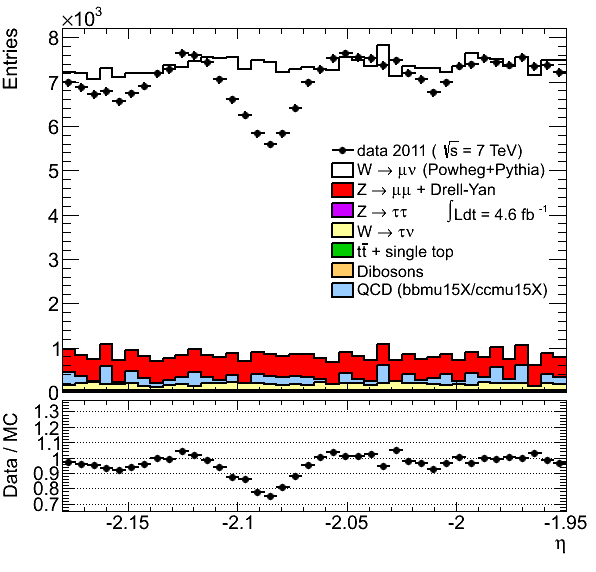
\includegraphics[width=0.66\textwidth]{dates/20130306/figures/etaphi/Widms_10_C_stack_l_eta_NEG} \\
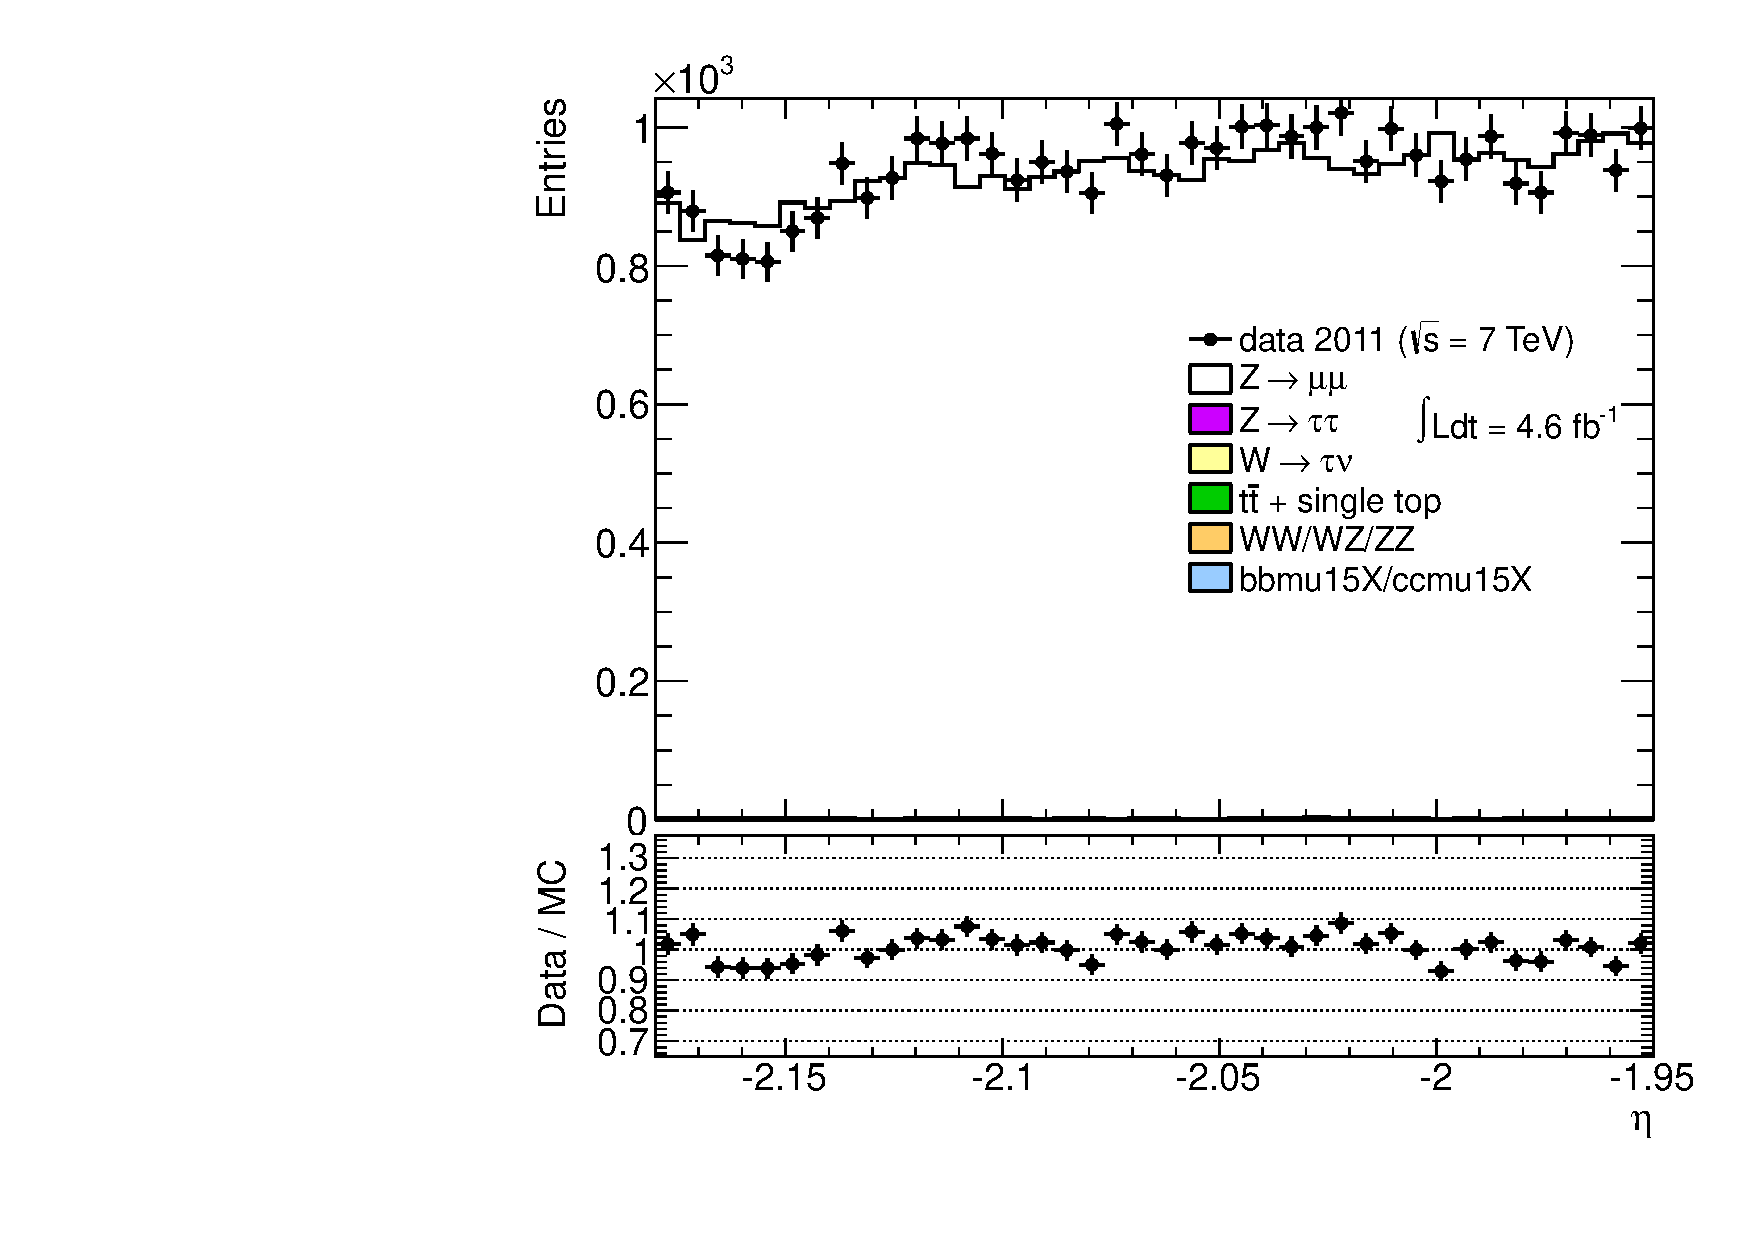
\includegraphics[width=0.66\textwidth]{dates/20130306/figures/etaphi/Zidms_10_C_stack_lN_eta_ALL.pdf}

\column{.5\textwidth}
A-side $\mu^{-}$ (top: W; bottom: Z)
\centering
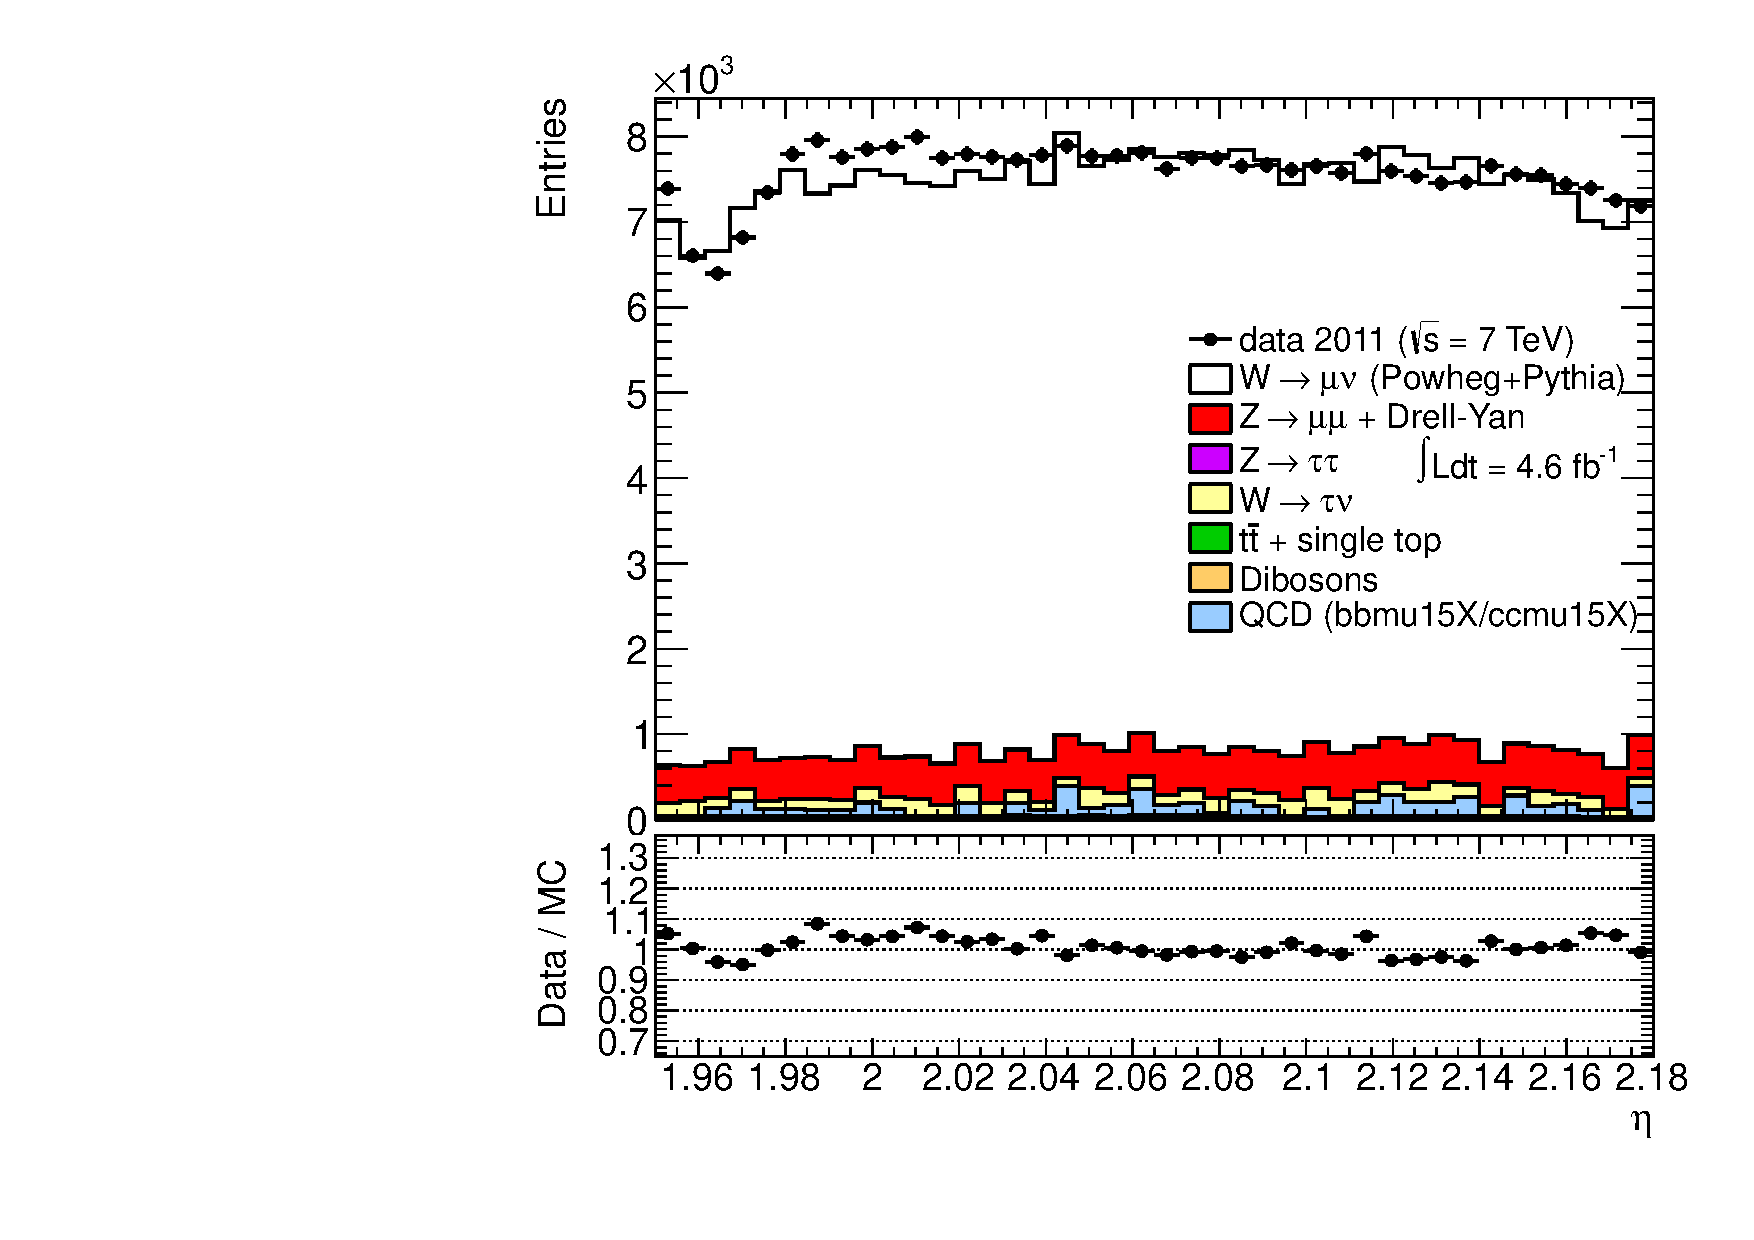
\includegraphics[width=0.66\textwidth]{dates/20130306/figures/etaphi/Widms_10_A_stack_l_eta_NEG} \\
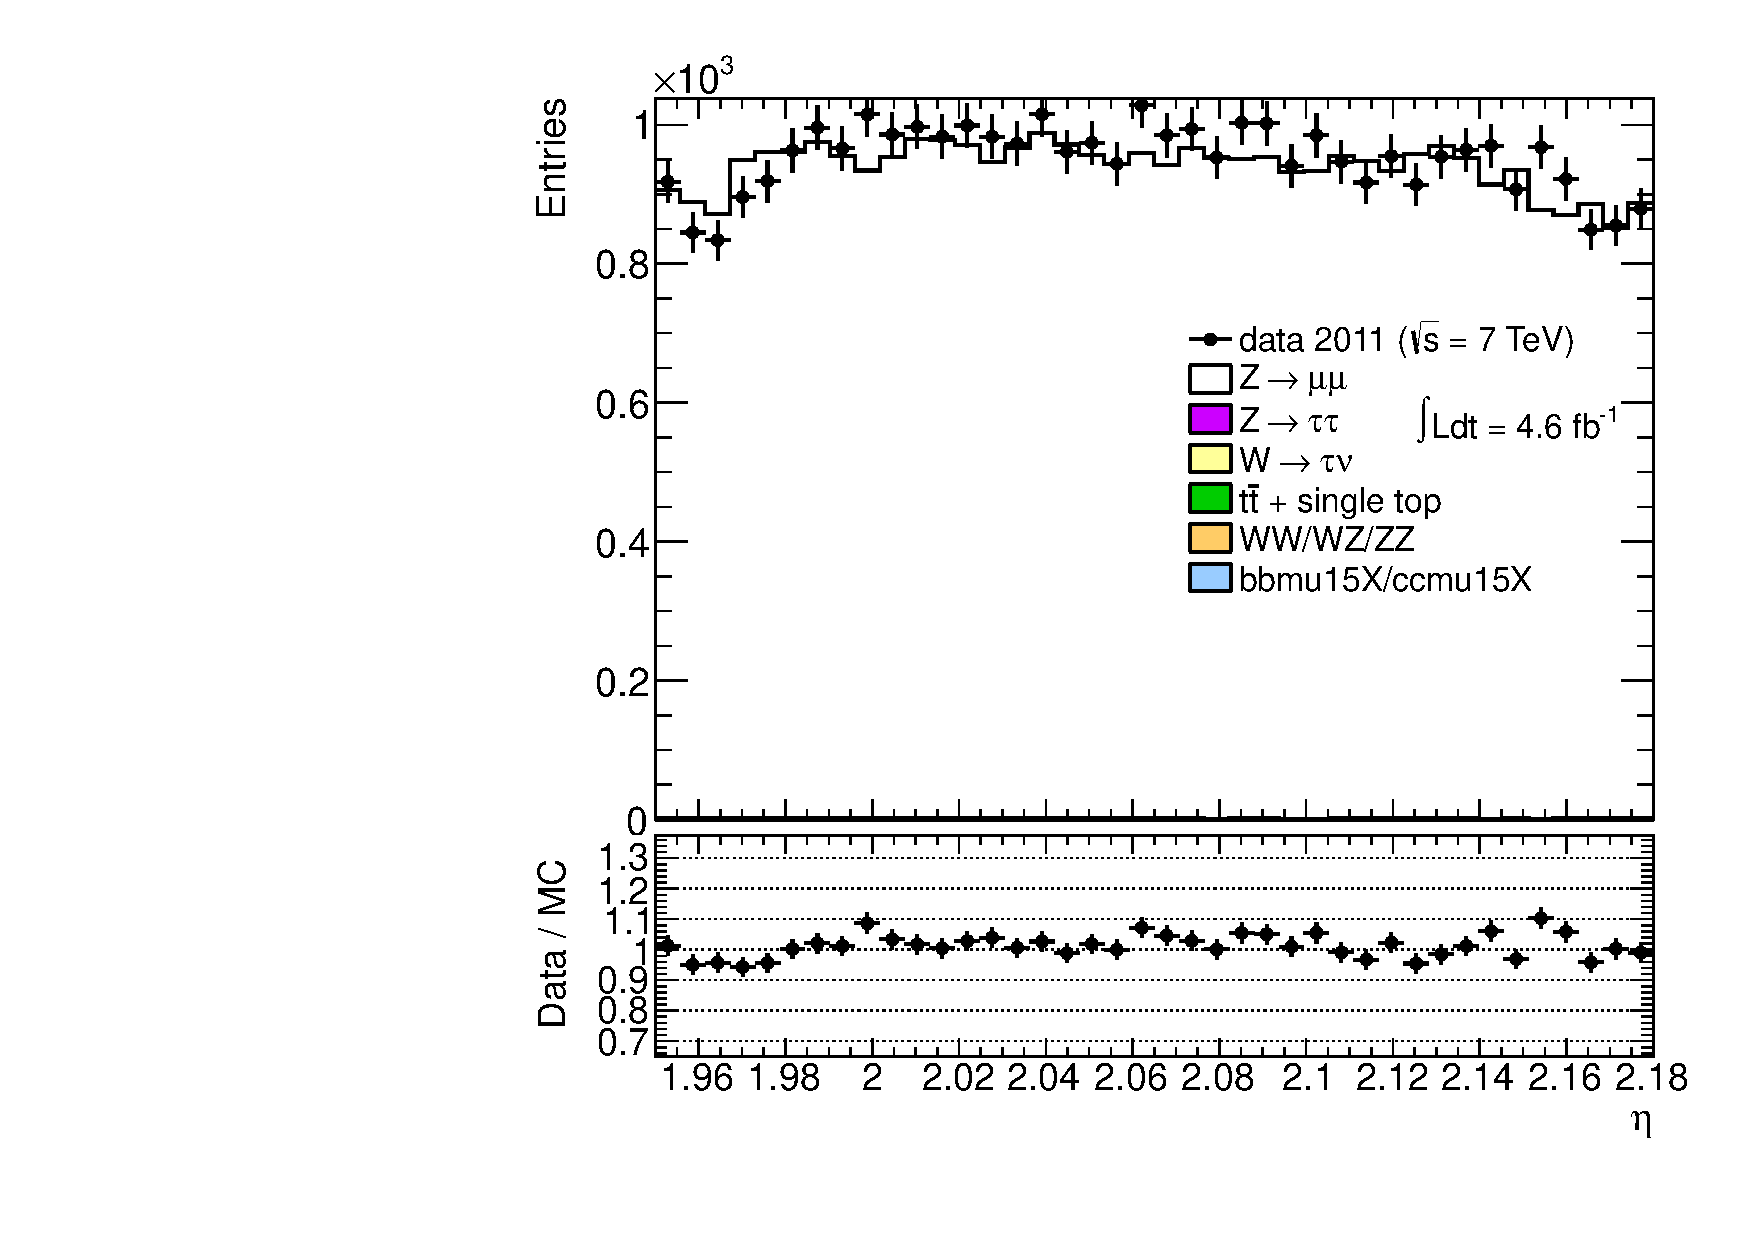
\includegraphics[width=0.66\textwidth]{dates/20130306/figures/etaphi/Zidms_10_A_stack_lN_eta_ALL.pdf} 

\cole
}


\only<19>{
What if we have very poorly reconstructed muons around the dip? \\
In that case, Z tag-and-probe and control plots would not see them \\
(because of the Z mass constraint) \\
Here, we use the muon pT measurement from ID only (in W channel), plus drop MET/WMT.
}

\only<20> {
\colb[T]

\column{.5\textwidth}
C-side $\mu^{-}$ (top: W; bottom: Z)
\centering
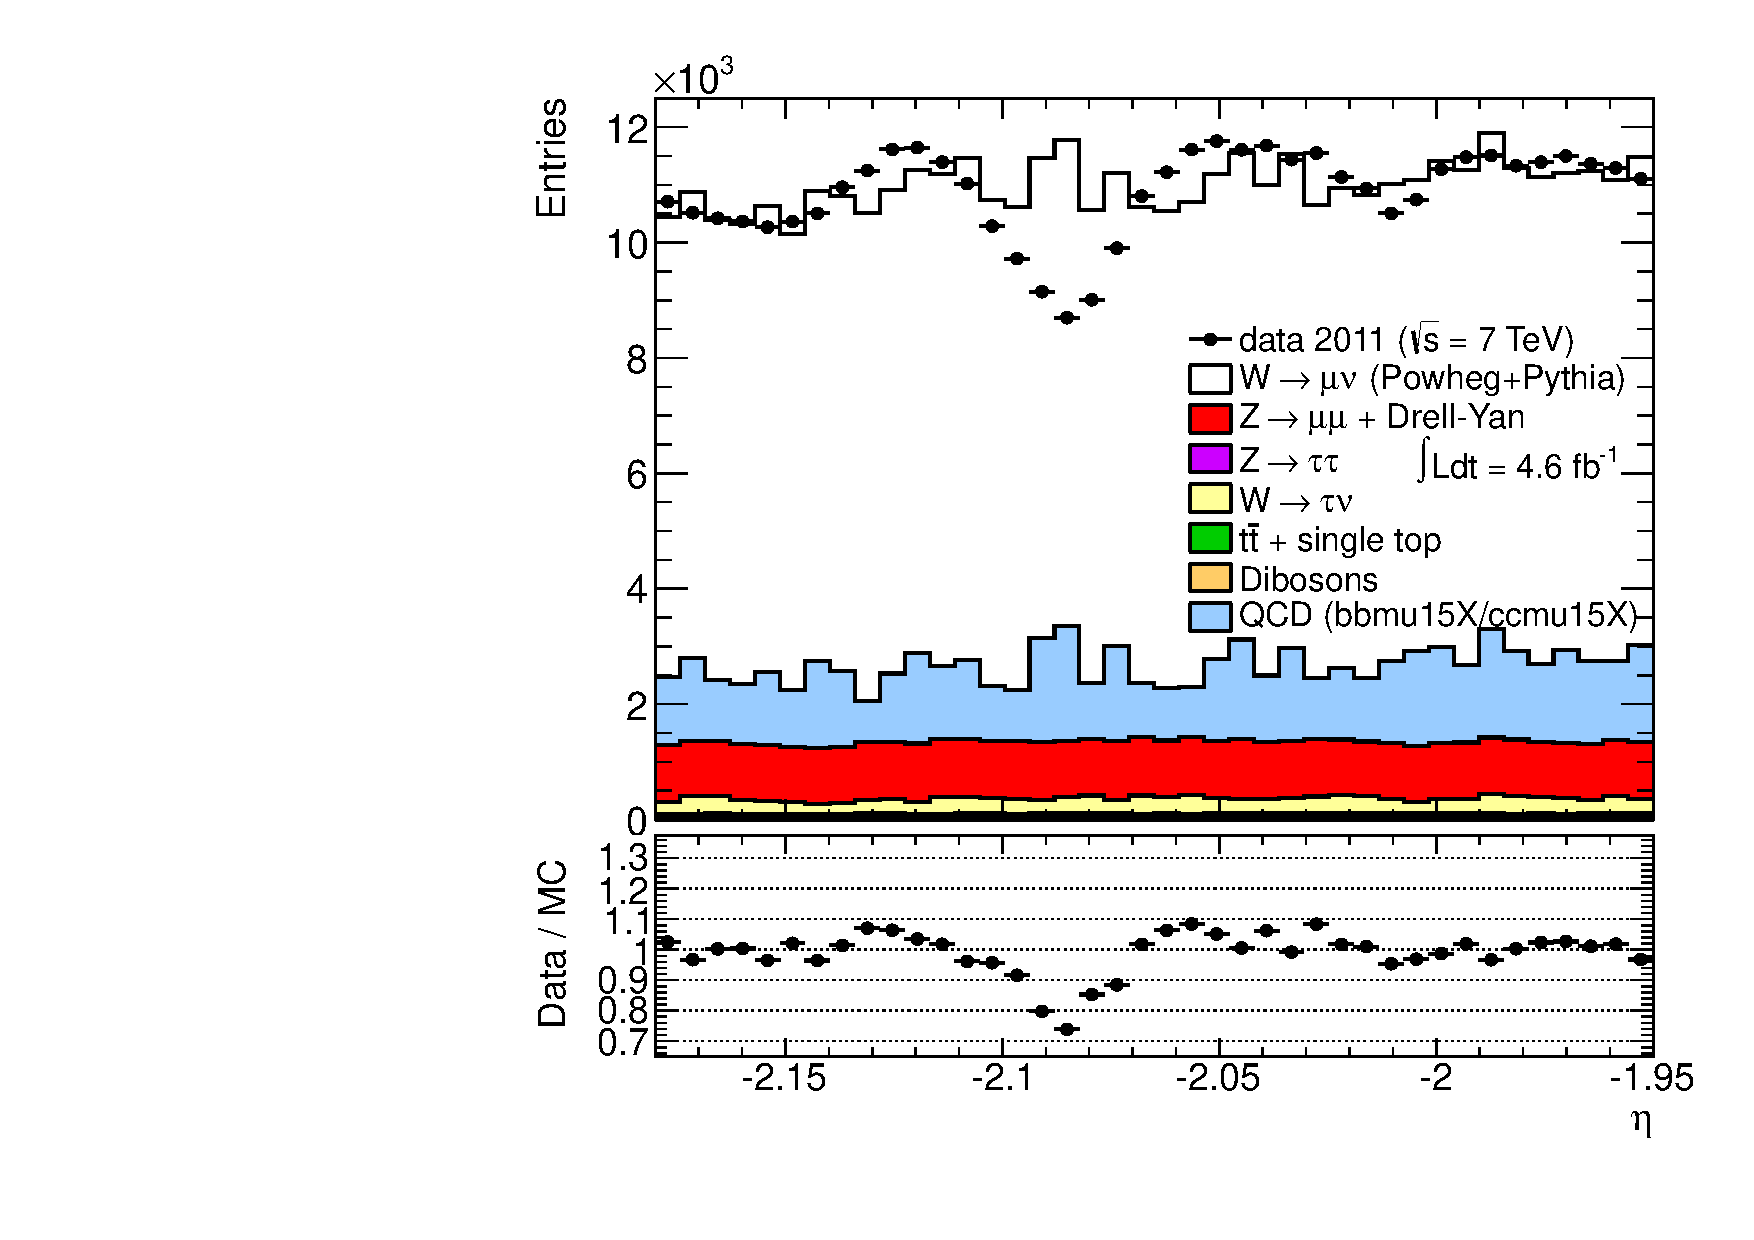
\includegraphics[width=0.66\textwidth]{dates/20130306/figures/etaphi/Wnometmtid_10_C_stack_l_eta_NEG} \\
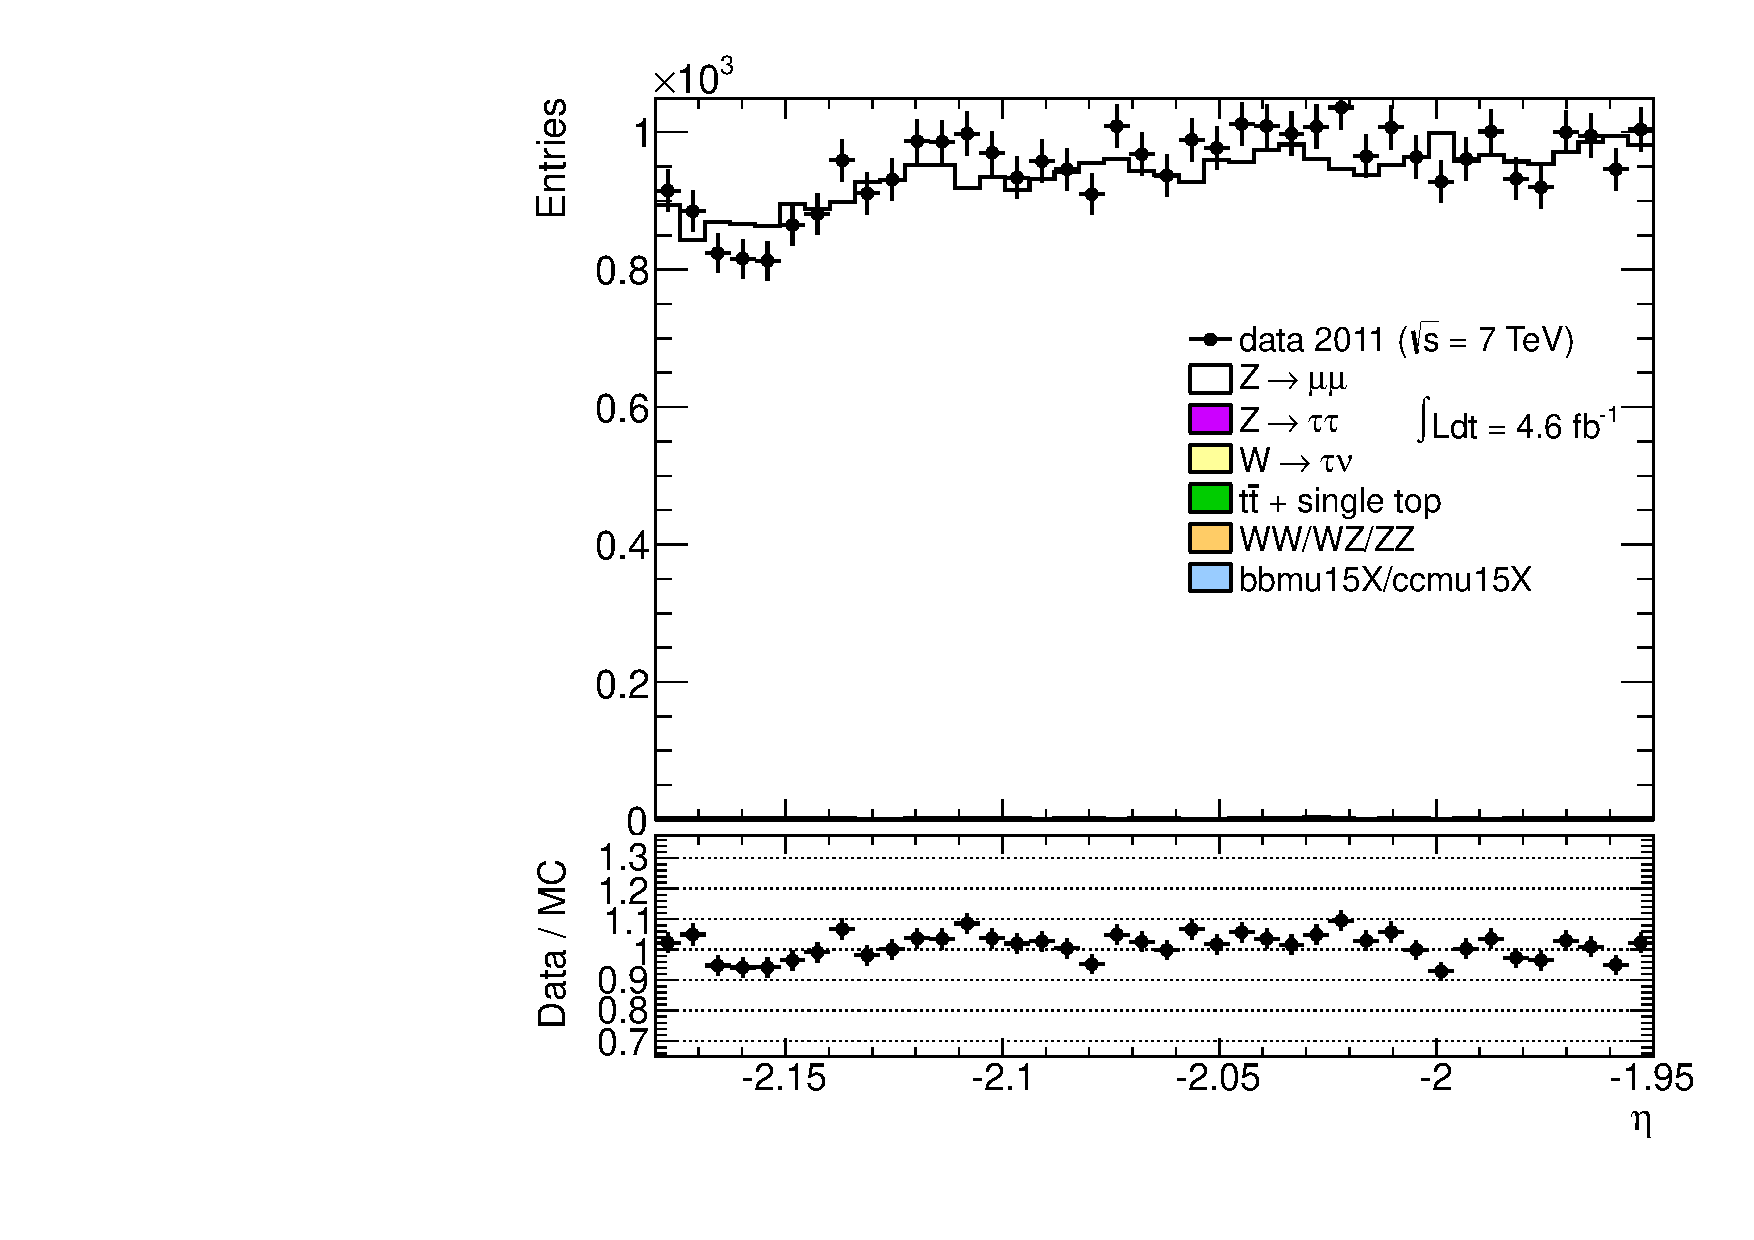
\includegraphics[width=0.66\textwidth]{dates/20130306/figures/etaphi/Z_10_C_stack_lN_eta_ALL.pdf}

\column{.5\textwidth}
A-side $\mu^{-}$ (top: W; bottom: Z)
\centering
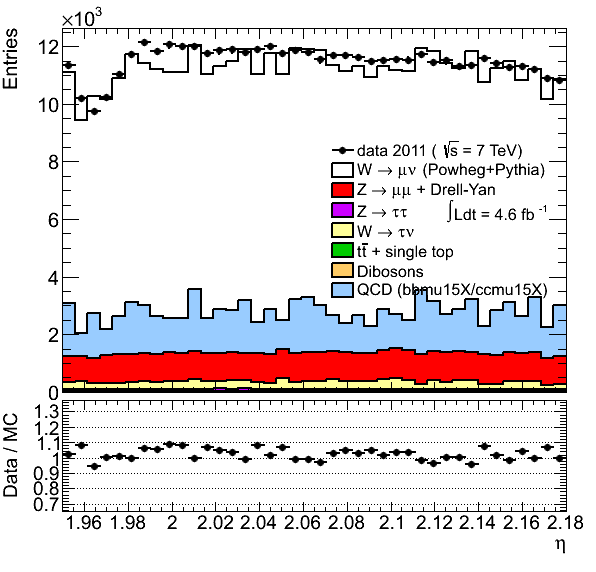
\includegraphics[width=0.66\textwidth]{dates/20130306/figures/etaphi/Wnometmtid_10_A_stack_l_eta_NEG} \\
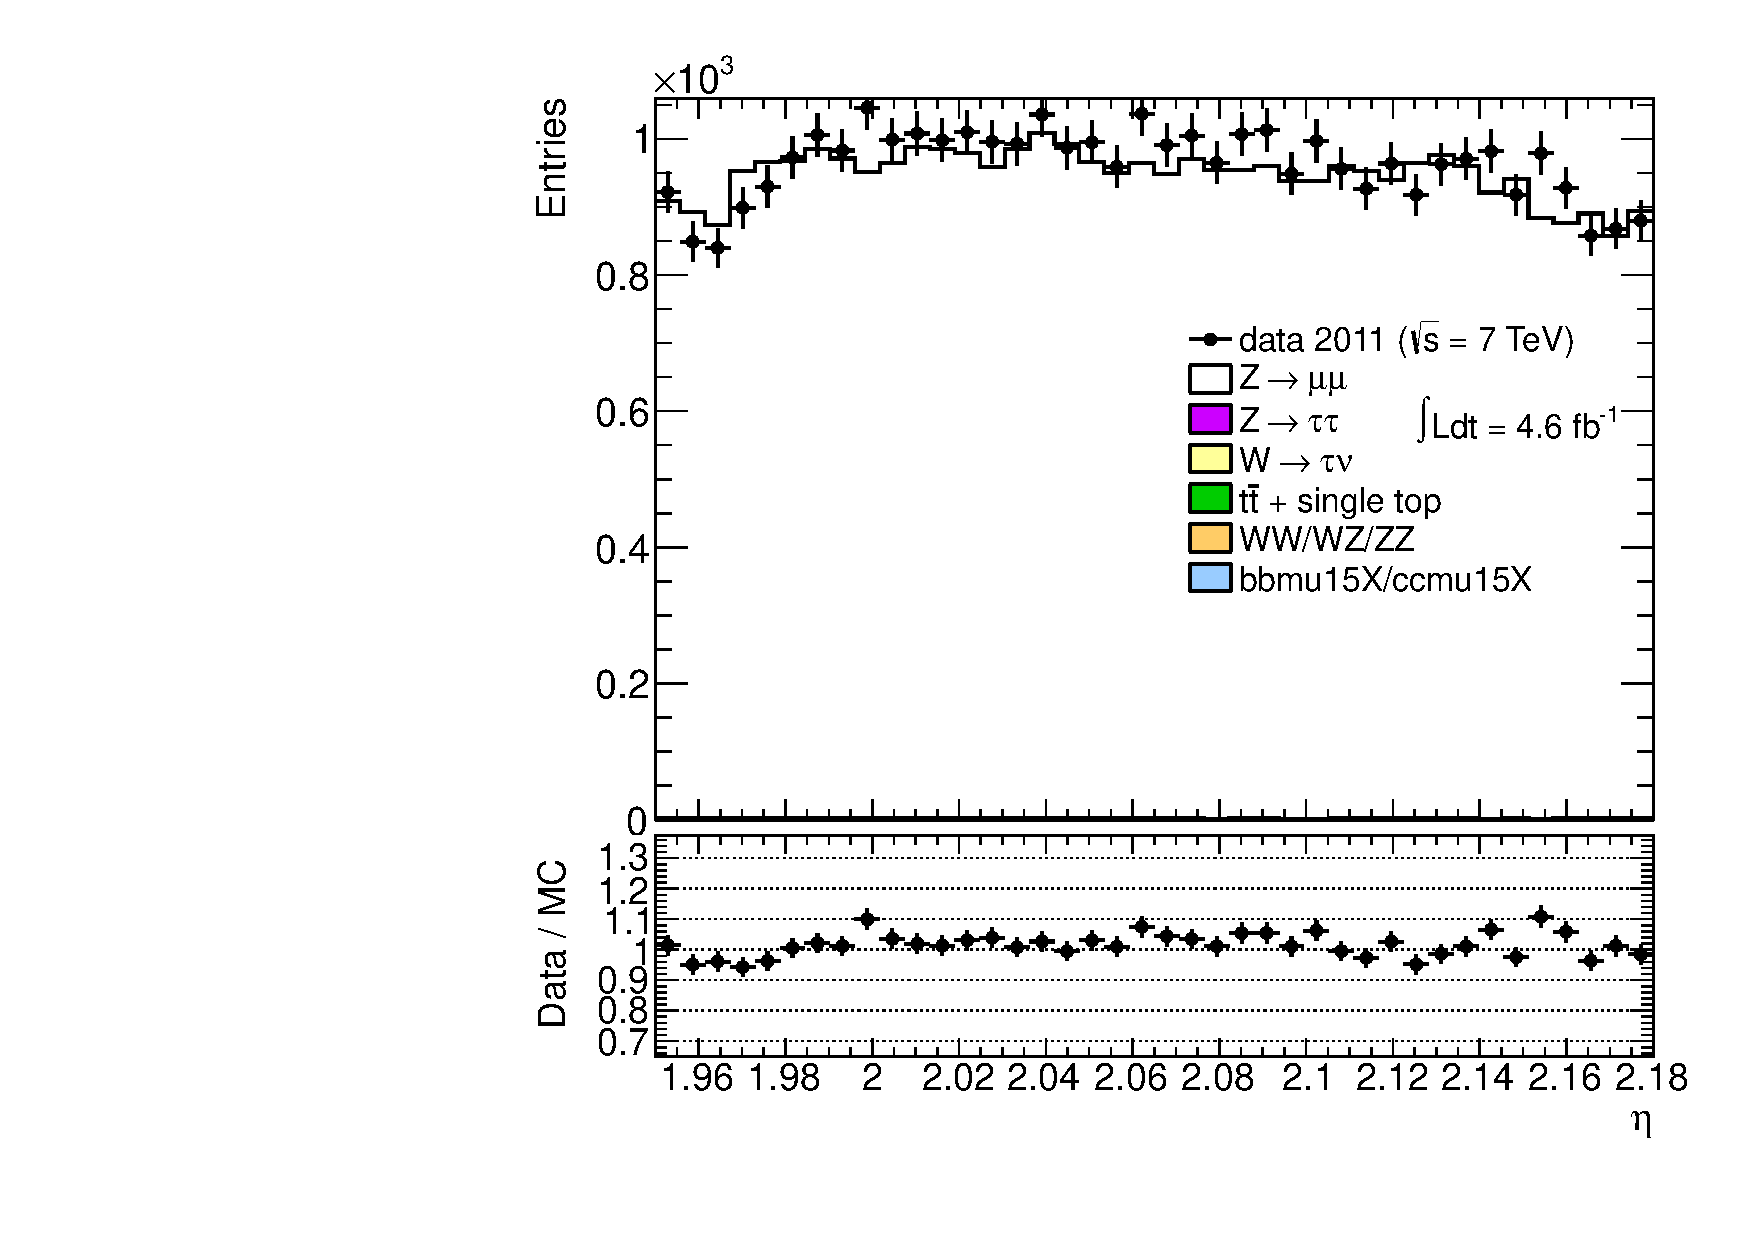
\includegraphics[width=0.66\textwidth]{dates/20130306/figures/etaphi/Z_10_A_stack_lN_eta_ALL.pdf} 

\cole
}


\only<21>{
What if we have very poorly reconstructed muons around the dip? \\
In that case, Z tag-and-probe and control plots would not see them \\
(because of the Z mass constraint) \\
Here, we completely drop the Z mass constraint
}

\only<22> {
\colb[T]

\column{.5\textwidth}
C-side $\mu^{-}$ (top: W; bottom: Z)
\centering
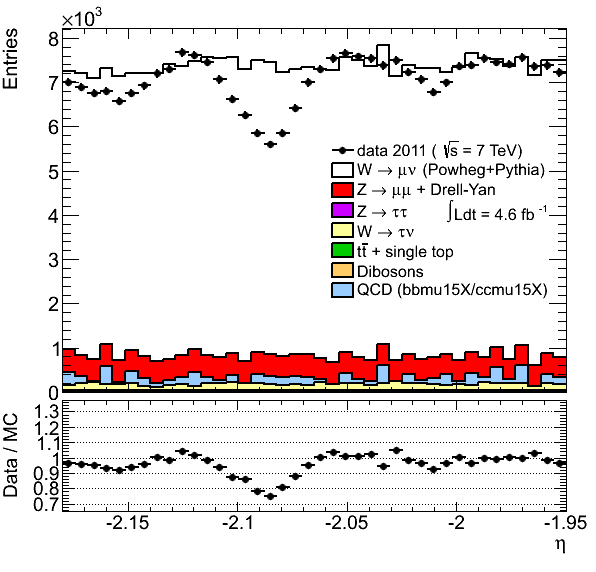
\includegraphics[width=0.66\textwidth]{dates/20130306/figures/etaphi/W_10_C_stack_l_eta_NEG} \\
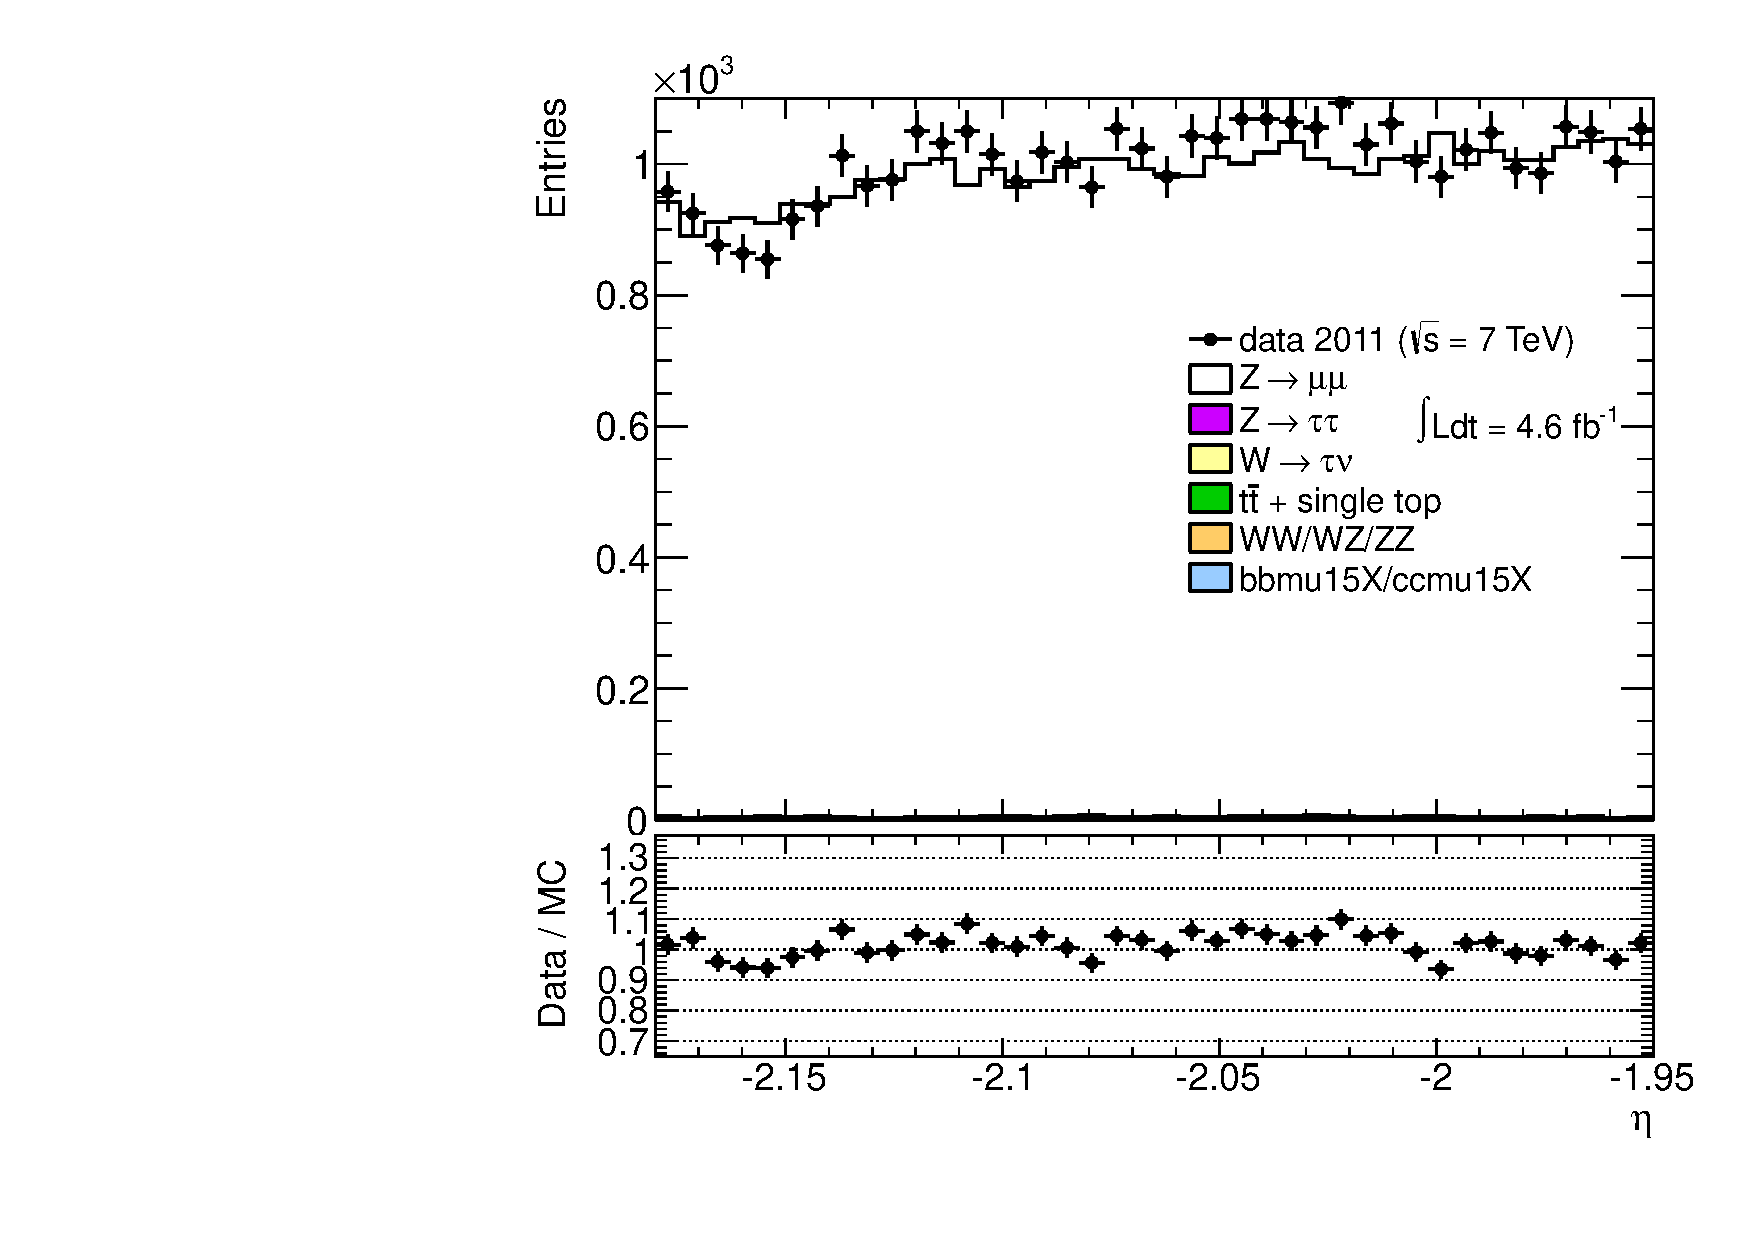
\includegraphics[width=0.66\textwidth]{dates/20130306/figures/etaphi/Znowind_10_C_stack_lN_eta_ALL.pdf}

\column{.5\textwidth}
A-side $\mu^{-}$ (top: W; bottom: Z)
\centering
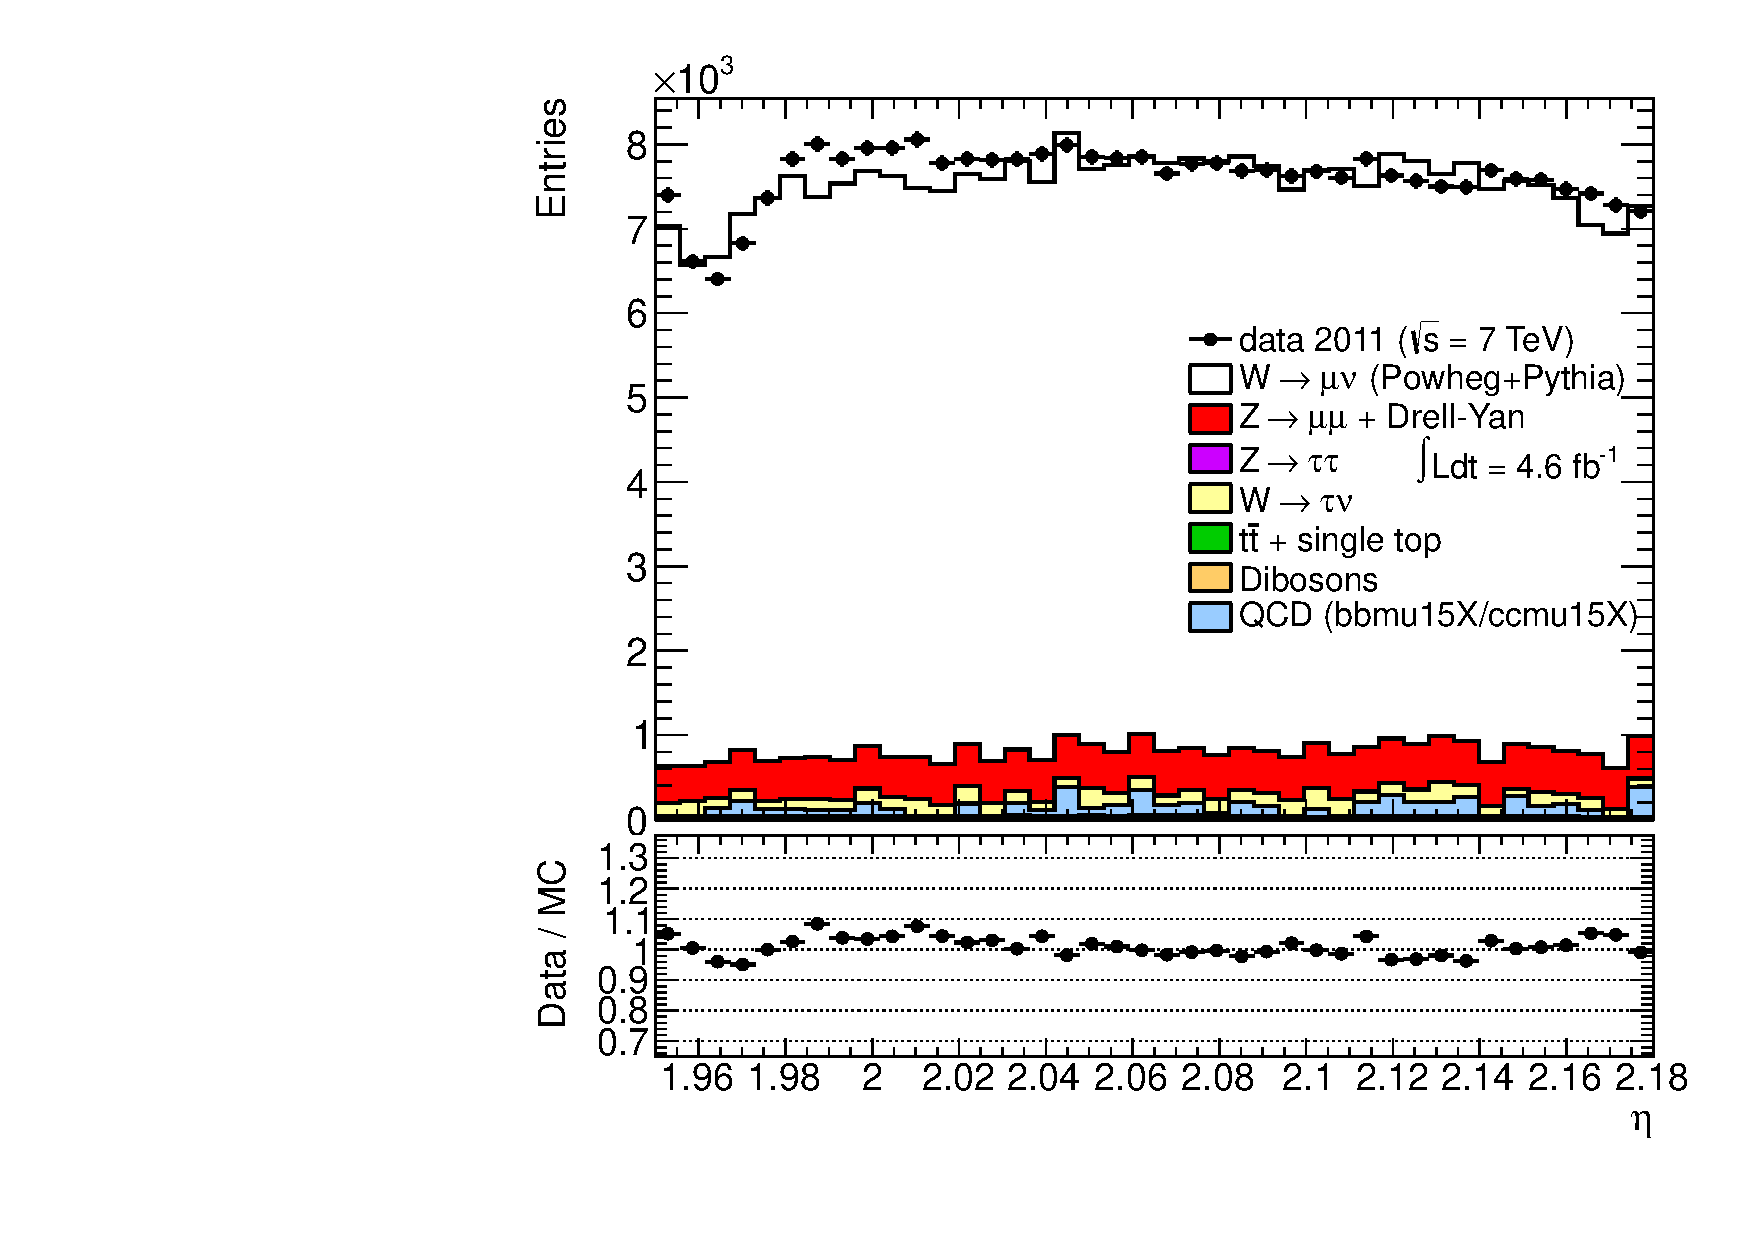
\includegraphics[width=0.66\textwidth]{dates/20130306/figures/etaphi/W_10_A_stack_l_eta_NEG} \\
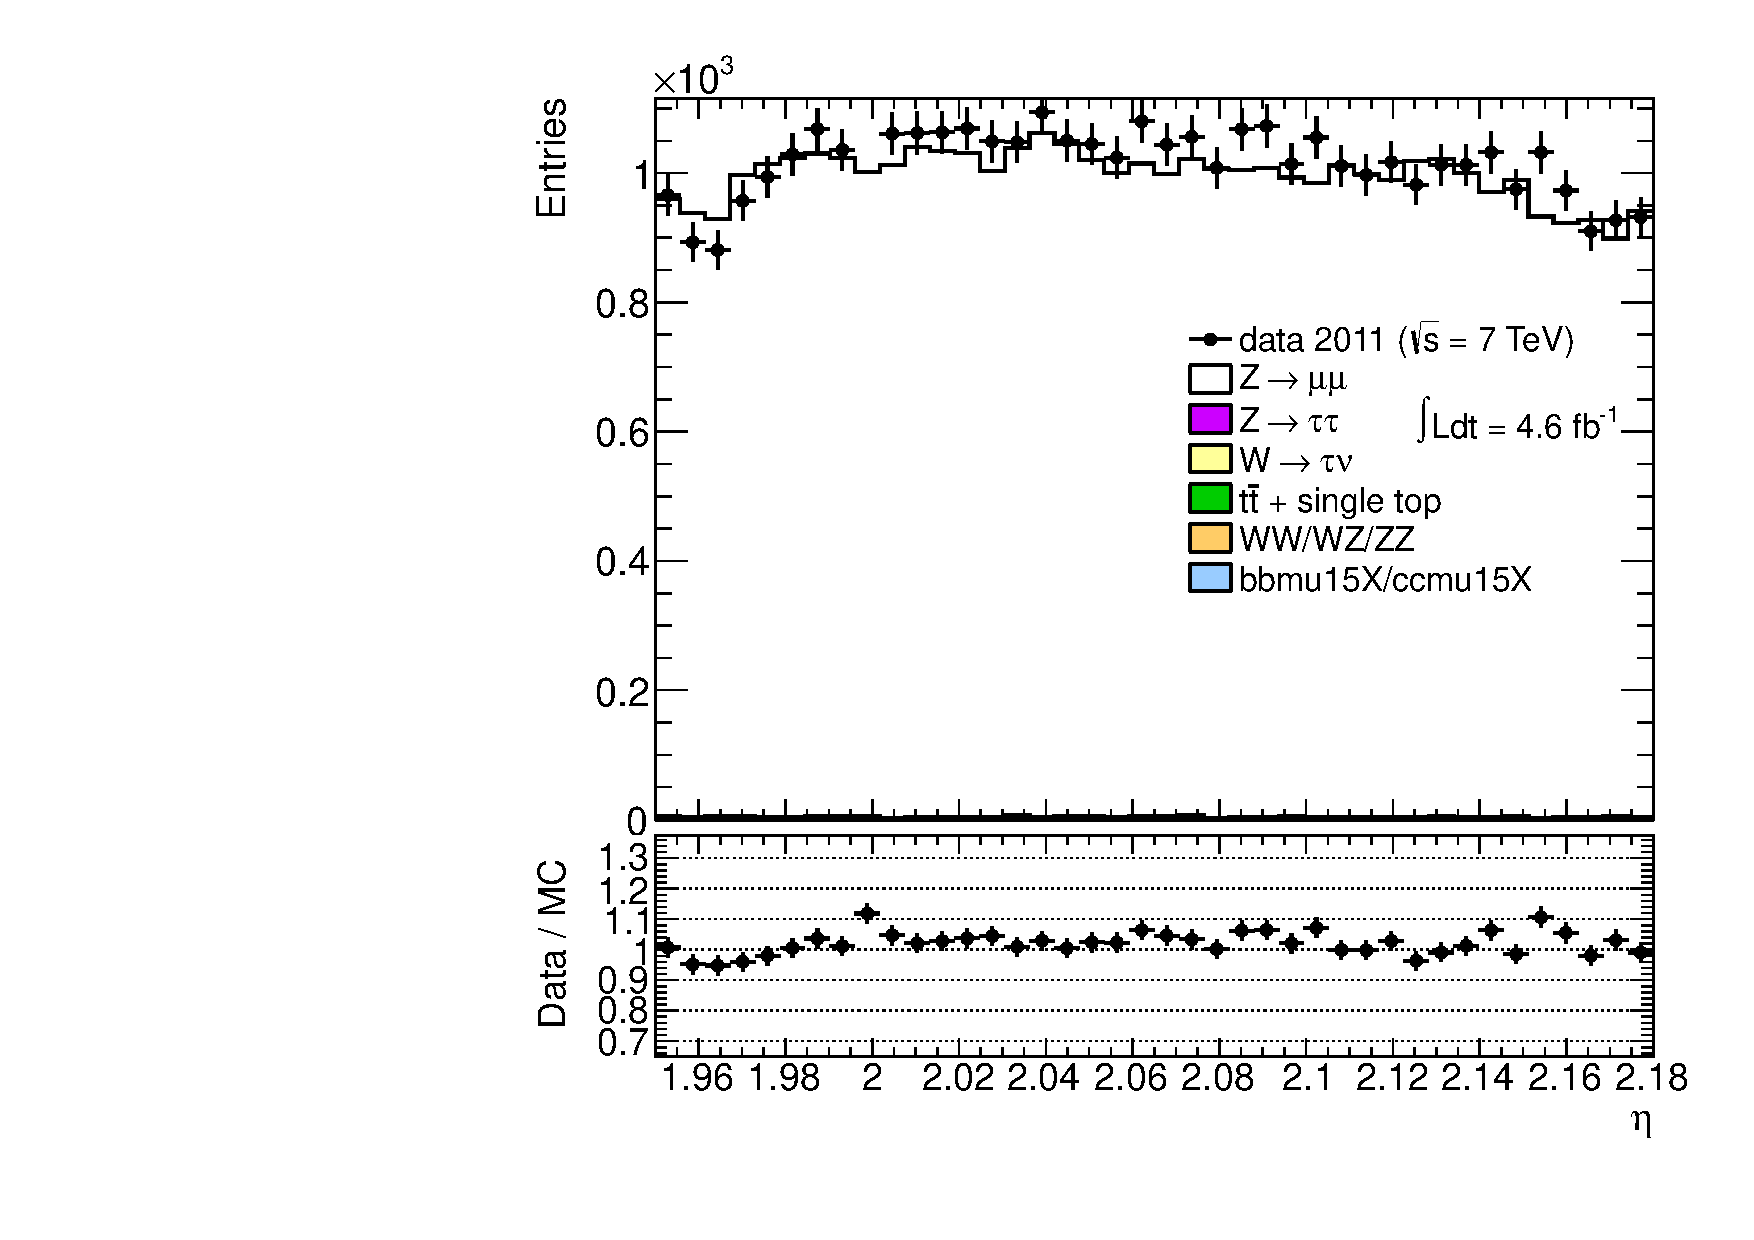
\includegraphics[width=0.66\textwidth]{dates/20130306/figures/etaphi/Znowind_10_A_stack_lN_eta_ALL.pdf} 

\cole
}


\only<23>{
What in the world could cause the dip in W selection? \\
Let's try dropping various cuts in the W selection. \\
Drop nmuons==1 cut (i.e. allow additional muons in an event).
}

\only<24> {
\colb[T]

\column{.5\textwidth}
C-side $\mu^{-}$ (top: W; bottom: Z)
\centering
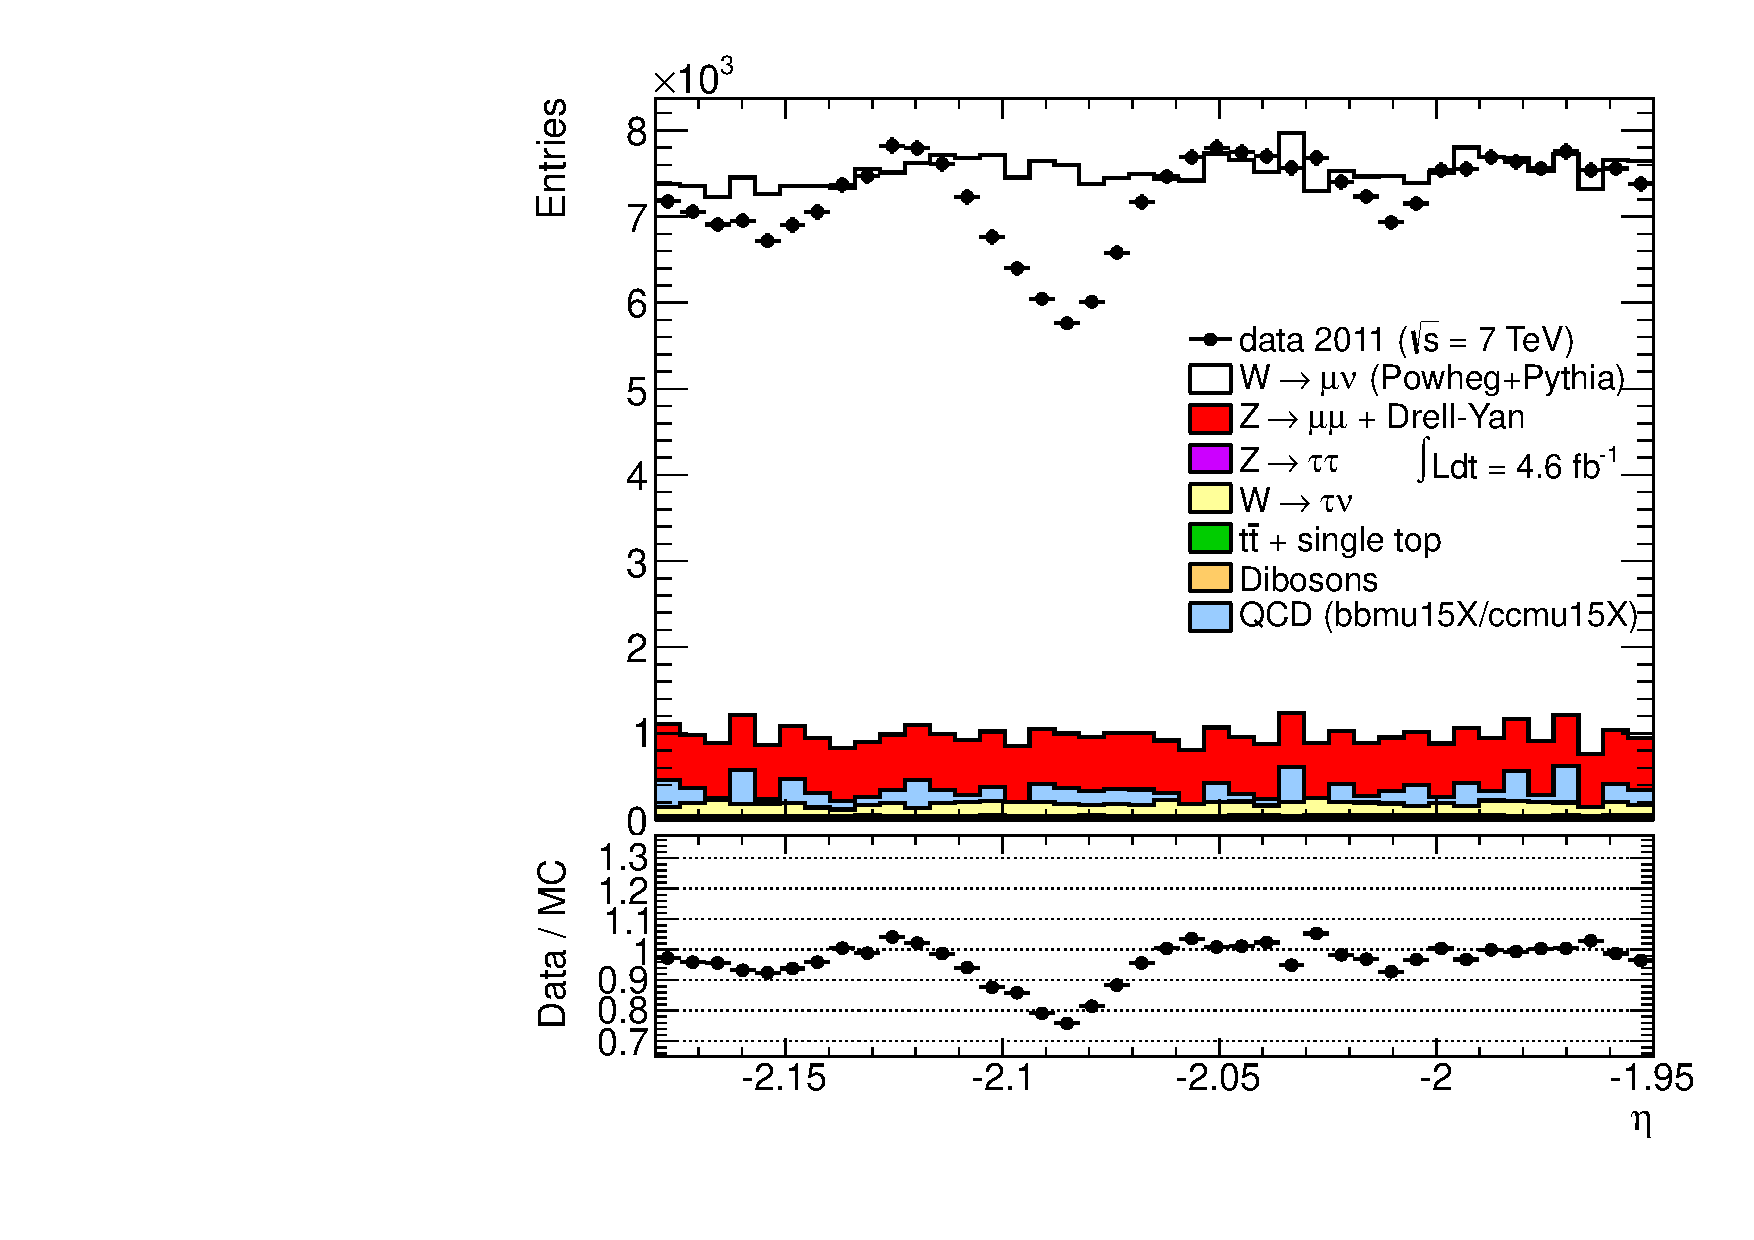
\includegraphics[width=0.66\textwidth]{dates/20130306/figures/etaphi/Wnonmu_10_C_stack_l_eta_NEG} \\
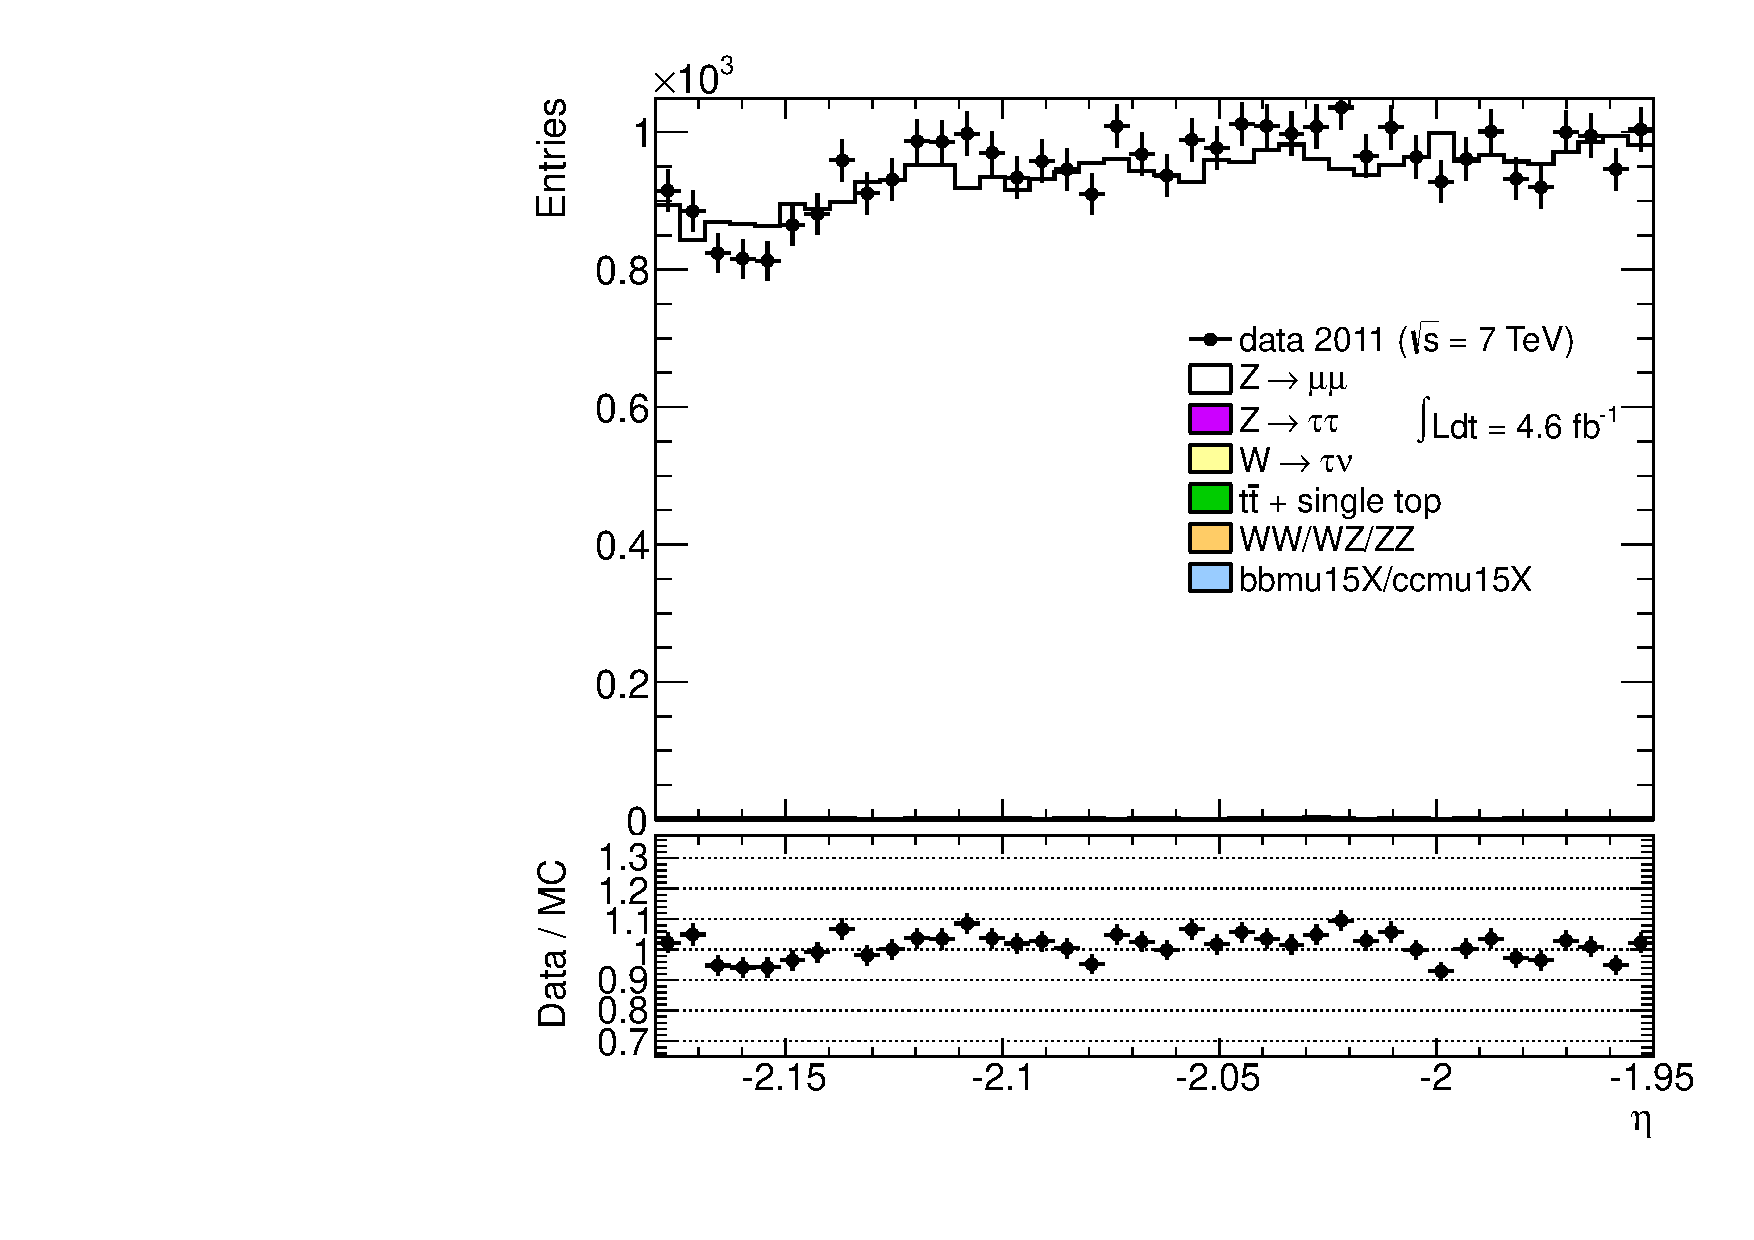
\includegraphics[width=0.66\textwidth]{dates/20130306/figures/etaphi/Z_10_C_stack_lN_eta_ALL.pdf}

\column{.5\textwidth}
A-side $\mu^{-}$ (top: W; bottom: Z)
\centering
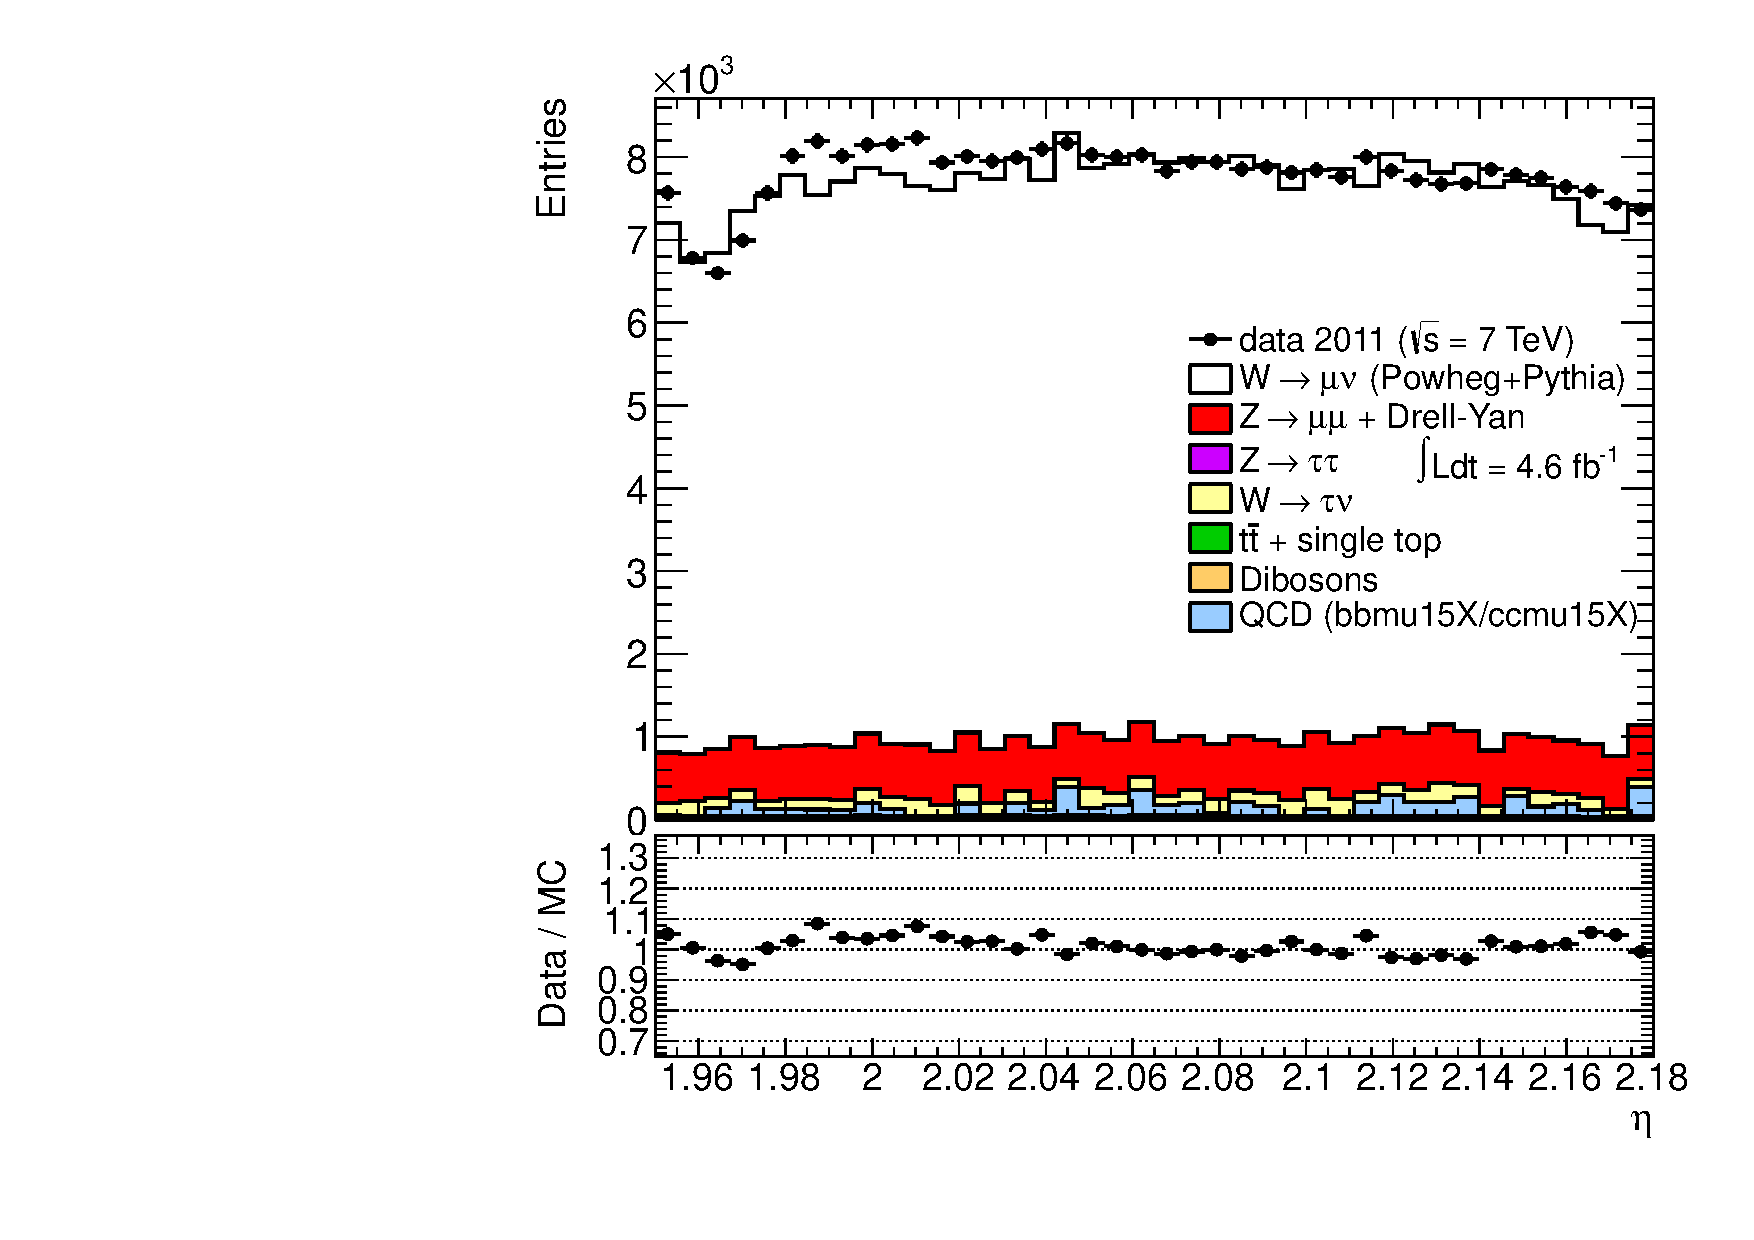
\includegraphics[width=0.66\textwidth]{dates/20130306/figures/etaphi/Wnonmu_10_A_stack_l_eta_NEG} \\
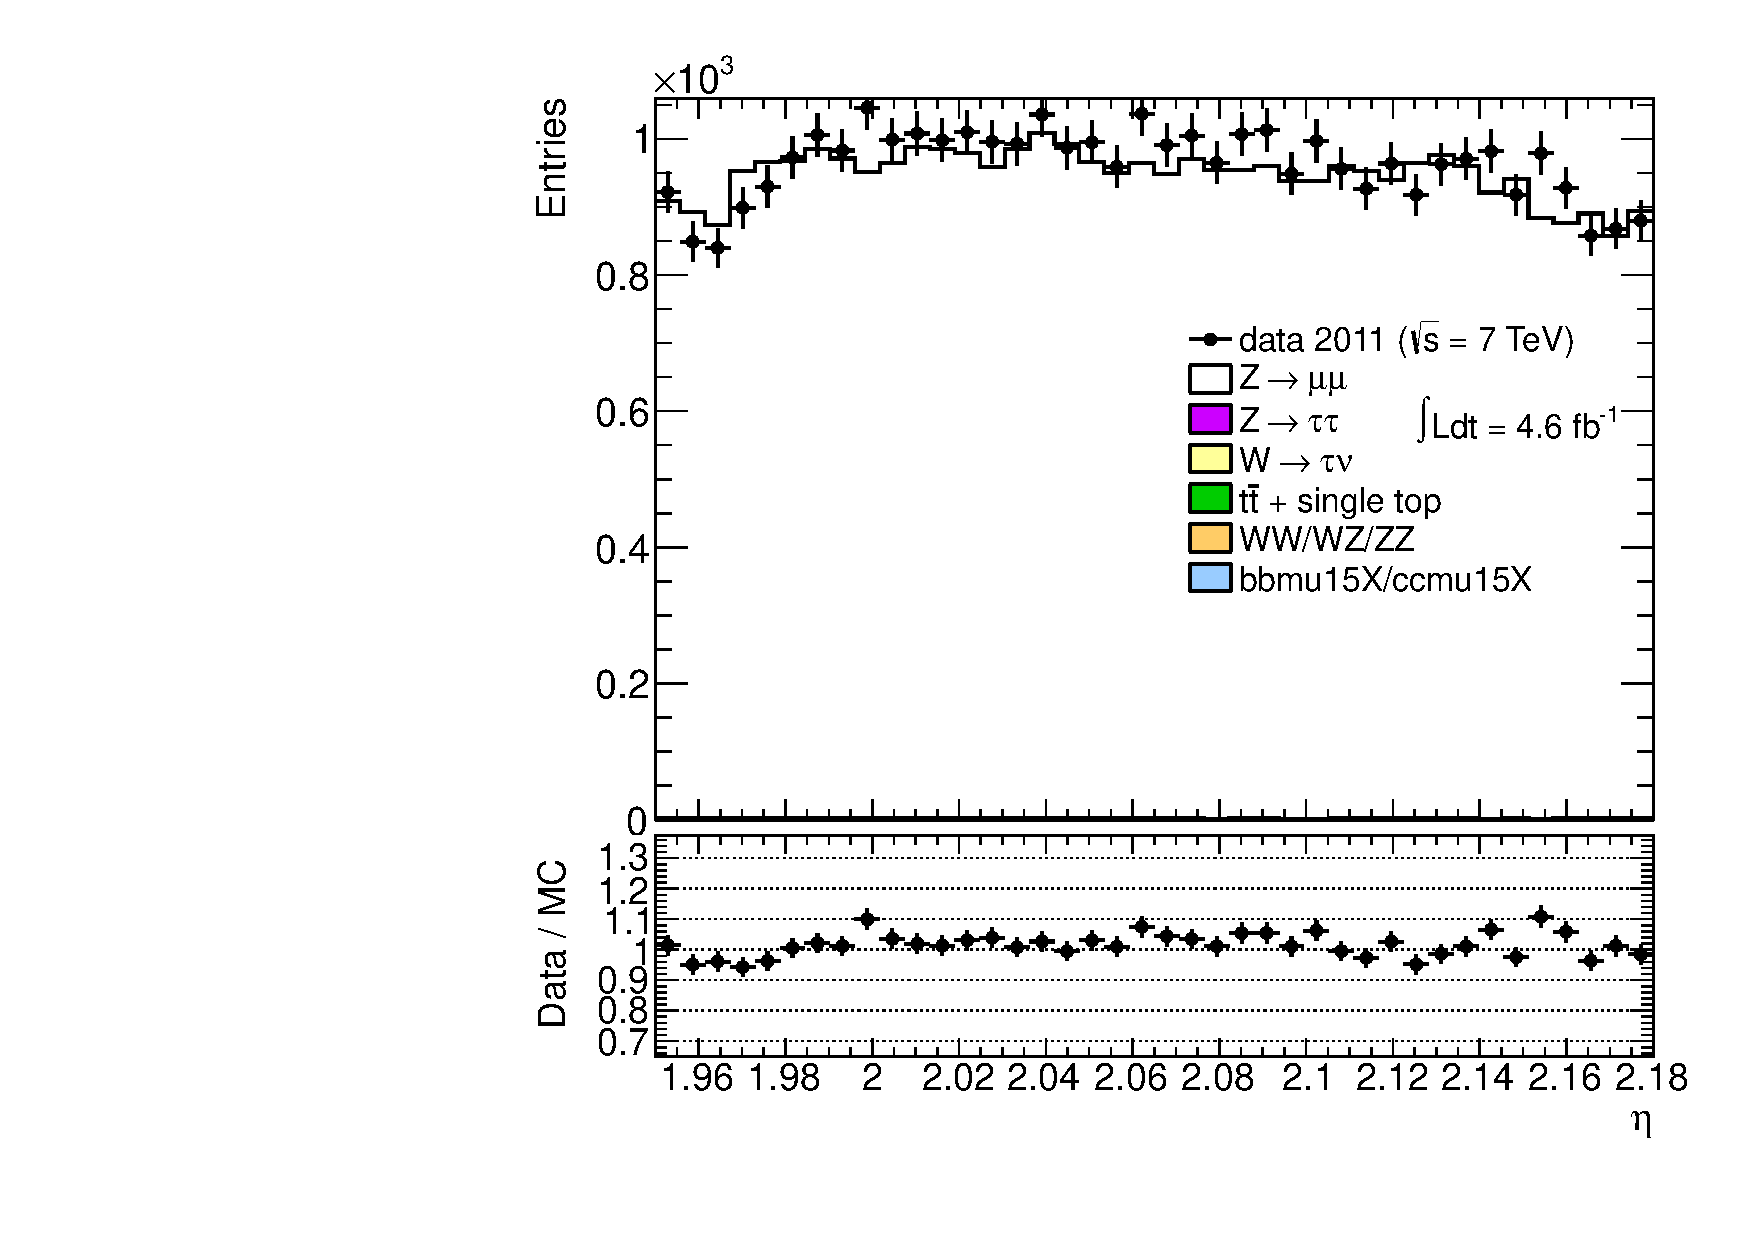
\includegraphics[width=0.66\textwidth]{dates/20130306/figures/etaphi/Z_10_A_stack_lN_eta_ALL.pdf} 

\cole
}


\only<25>{
What in the world could cause the dip in W selection? \\
Let's try dropping various cuts in the W selection. \\
Drop all cuts, except: one 15-GeV muon (MCP-quality)
}

\only<26> {
\colb[T]

\column{.5\textwidth}
C-side $\mu^{-}$ (top: W; bottom: Z)
\centering
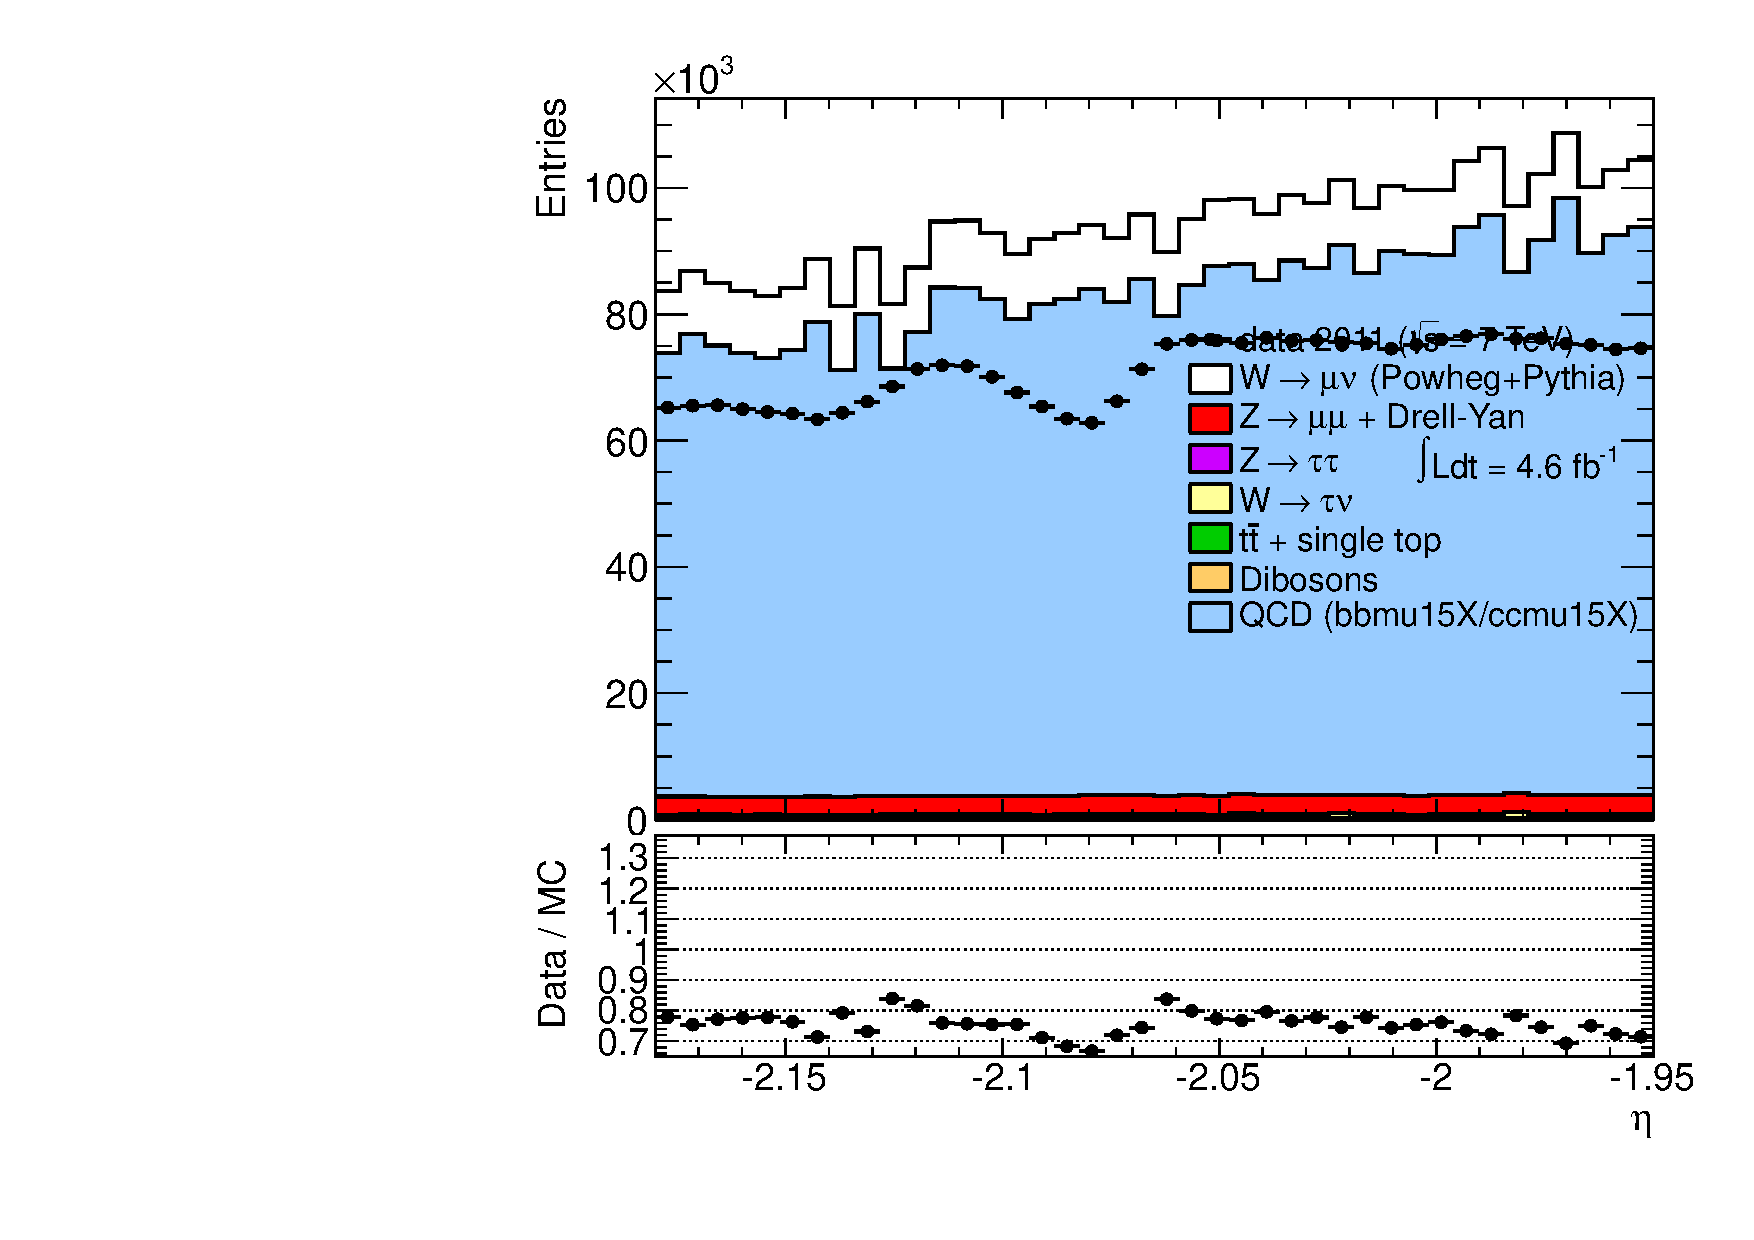
\includegraphics[width=0.66\textwidth]{dates/20130306/figures/etaphi/Wnocuts_10_C_stack_l_eta_NEG} \\
\includegraphics[width=0.66\textwidth]{dates/20130306/figures/etaphi/Z_10_C_stack_lN_eta_ALL.pdf}

\column{.5\textwidth}
A-side $\mu^{-}$ (top: W; bottom: Z)
\centering
\includegraphics[width=0.66\textwidth]{dates/20130306/figures/etaphi/Wnocuts_10_A_stack_l_eta_NEG} \\
\includegraphics[width=0.66\textwidth]{dates/20130306/figures/etaphi/Z_10_A_stack_lN_eta_ALL.pdf} 

\cole
}


\only<27>{
OK, the dip is still seen. Is there a bug in my W ntuple? \\
Let's use my W ntuple, but force nmuons==2. This should select mostly Z events. \\
(in this test, no Z mass or opposite charges constraint is applied)
}

\only<28> {
\colb[T]

\column{.5\textwidth}
C-side $\mu^{-}$ (top: W; bottom: Z)
\centering
\includegraphics[width=0.66\textwidth]{dates/20130306/figures/etaphi/Wzlike_10_C_stack_l_eta_NEG} \\
\includegraphics[width=0.66\textwidth]{dates/20130306/figures/etaphi/Z_10_C_stack_lN_eta_ALL.pdf}

\column{.5\textwidth}
A-side $\mu^{-}$ (top: W; bottom: Z)
\centering
\includegraphics[width=0.66\textwidth]{dates/20130306/figures/etaphi/Wzlike_10_A_stack_l_eta_NEG} \\
\includegraphics[width=0.66\textwidth]{dates/20130306/figures/etaphi/Z_10_A_stack_lN_eta_ALL.pdf} 

\cole
}


\only<29>{
In all Z plots, we require that the tag muon has to trigger, too. \\
(but it's allowed to be anywhere) \\
Let's drop the requirement that the tag muon triggered. \\
We expect (and see) no changes in the Z plot...

}

\only<30> {
\colb[T]

\column{.5\textwidth}
C-side $\mu^{-}$ (top: W; bottom: Z)
\centering
\includegraphics[width=0.66\textwidth]{dates/20130306/figures/etaphi/W_10_C_stack_l_eta_NEG} \\
\includegraphics[width=0.66\textwidth]{dates/20130306/figures/etaphi/Ztprobe_10_C_stack_lN_eta_ALL.pdf}

\column{.5\textwidth}
A-side $\mu^{-}$ (top: W; bottom: Z)
\centering
\includegraphics[width=0.66\textwidth]{dates/20130306/figures/etaphi/W_10_A_stack_l_eta_NEG} \\
\includegraphics[width=0.66\textwidth]{dates/20130306/figures/etaphi/Ztprobe_10_A_stack_lN_eta_ALL.pdf} 

\cole
}


\only<31>{
In all Z plots, we require that the tag muon has to trigger, too. \\
(but it's allowed to be anywhere) \\
Let's drop the requirement that the tag muon triggered. \\
Here, we also require that the Z probe muon (the one we're plotting) \\
matches the trigger in a more narrow cone of 0.05 (vs standard 0.2)

}

\only<32> {
\colb[T]

\column{.5\textwidth}
C-side $\mu^{-}$ (top: W; bottom: Z)
\centering
\includegraphics[width=0.66\textwidth]{dates/20130306/figures/etaphi/W_10_C_stack_l_eta_NEG} \\
\includegraphics[width=0.66\textwidth]{dates/20130306/figures/etaphi/Ztprobet_10_C_stack_lN_eta_ALL.pdf}

\column{.5\textwidth}
A-side $\mu^{-}$ (top: W; bottom: Z)
\centering
\includegraphics[width=0.66\textwidth]{dates/20130306/figures/etaphi/W_10_A_stack_l_eta_NEG} \\
\includegraphics[width=0.66\textwidth]{dates/20130306/figures/etaphi/Ztprobet_10_A_stack_lN_eta_ALL.pdf} 

\cole
}


\only<33>{
Let's examine period dependence of the dip in W. \\
Start with period(s) D-H.
}

\only<34> {
\colb[T]

\column{.5\textwidth}
C-side $\mu^{-}$ (top: W; bottom: Z)
\centering
\includegraphics[width=0.66\textwidth]{dates/20130306/figures/etaphi/WpDtoH_10_C_stack_l_eta_NEG} \\
\includegraphics[width=0.66\textwidth]{dates/20130306/figures/etaphi/Z_10_C_stack_lN_eta_ALL.pdf}

\column{.5\textwidth}
A-side $\mu^{-}$ (top: W; bottom: Z)
\centering
\includegraphics[width=0.66\textwidth]{dates/20130306/figures/etaphi/WpDtoH_10_A_stack_l_eta_NEG} \\
\includegraphics[width=0.66\textwidth]{dates/20130306/figures/etaphi/Z_10_A_stack_lN_eta_ALL.pdf} 

\cole
}

\only<35>{
AHA! there is no dip. Let's see when it appears \\
Let's examine period dependence of the dip in W. \\
Period(s) I only.
}

\only<36> {
\colb[T]

\column{.5\textwidth}
C-side $\mu^{-}$ (top: W; bottom: Z)
\centering
\includegraphics[width=0.66\textwidth]{dates/20130306/figures/etaphi/WpItoI_10_C_stack_l_eta_NEG} \\
\includegraphics[width=0.66\textwidth]{dates/20130306/figures/etaphi/Z_10_C_stack_lN_eta_ALL.pdf}

\column{.5\textwidth}
A-side $\mu^{-}$ (top: W; bottom: Z)
\centering
\includegraphics[width=0.66\textwidth]{dates/20130306/figures/etaphi/WpItoI_10_A_stack_l_eta_NEG} \\
\includegraphics[width=0.66\textwidth]{dates/20130306/figures/etaphi/Z_10_A_stack_lN_eta_ALL.pdf} 

\cole
}


\only<37>{
AHA! the dip is already present \red{in period I}.
Let's examine period dependence of the dip in W. \\
Period(s) I-K.
}

\only<38> {
\colb[T]

\column{.5\textwidth}
C-side $\mu^{-}$ (top: W; bottom: Z)
\centering
\includegraphics[width=0.66\textwidth]{dates/20130306/figures/etaphi/WpItoK_10_C_stack_l_eta_NEG} \\
\includegraphics[width=0.66\textwidth]{dates/20130306/figures/etaphi/Z_10_C_stack_lN_eta_ALL.pdf}

\column{.5\textwidth}
A-side $\mu^{-}$ (top: W; bottom: Z)
\centering
\includegraphics[width=0.66\textwidth]{dates/20130306/figures/etaphi/WpItoK_10_A_stack_l_eta_NEG} \\
\includegraphics[width=0.66\textwidth]{dates/20130306/figures/etaphi/Z_10_A_stack_lN_eta_ALL.pdf} 

\cole
}


\only<39>{
Let's examine period dependence of the dip in W. \\
Period(s) L.
}

\only<40> {
\colb[T]

\column{.5\textwidth}
C-side $\mu^{-}$ (top: W; bottom: Z)
\centering
\includegraphics[width=0.66\textwidth]{dates/20130306/figures/etaphi/WpLtoL_10_C_stack_l_eta_NEG} \\
\includegraphics[width=0.66\textwidth]{dates/20130306/figures/etaphi/Z_10_C_stack_lN_eta_ALL.pdf}

\column{.5\textwidth}
A-side $\mu^{-}$ (top: W; bottom: Z)
\centering
\includegraphics[width=0.66\textwidth]{dates/20130306/figures/etaphi/WpLtoL_10_A_stack_l_eta_NEG} \\
\includegraphics[width=0.66\textwidth]{dates/20130306/figures/etaphi/Z_10_A_stack_lN_eta_ALL.pdf} 

\cole
}


\only<41>{
Let's examine period dependence of the dip in W. \\
Period(s) M.
}

\only<42> {
\colb[T]

\column{.5\textwidth}
C-side $\mu^{-}$ (top: W; bottom: Z)
\centering
\includegraphics[width=0.66\textwidth]{dates/20130306/figures/etaphi/WpMtoM_10_C_stack_l_eta_NEG} \\
\includegraphics[width=0.66\textwidth]{dates/20130306/figures/etaphi/Z_10_C_stack_lN_eta_ALL.pdf}

\column{.5\textwidth}
A-side $\mu^{-}$ (top: W; bottom: Z)
\centering
\includegraphics[width=0.66\textwidth]{dates/20130306/figures/etaphi/WpMtoM_10_A_stack_l_eta_NEG} \\
\includegraphics[width=0.66\textwidth]{dates/20130306/figures/etaphi/Z_10_A_stack_lN_eta_ALL.pdf} 

\cole
}


\only<43>{
 Conclusions: \\
 \iteb
 \item Whenever we see A/C disagreements in a particular bin, we also see a funny $\eta$ dip
 \item See plots inside all other measurements $\eta$ bins are in the appendix
 \item Made attempts to introduce the dip in Z events, or remove in W events
 \iteb
 \item All kinematic and quality cuts have no effect
 \item Dip in W is absent before period I, but present thereafter
 \iteb
 \item Doesn't quite align with shift from mu18MG to mu18MGmedium, which happened \red{in the end of period I}.
 \item I will test other triggers, such as the non-MG version of EFmu18.
 \itee
 \item Dip disappears whenever there is a second tag muon (even if the probe is required to match trigger!)
 \iteb
 \item This makes me suspicious of trigger matching machinery? Maybe requiring a matching cone of 0.2 does not mean that the trigger actually fired in the DAQ?
 \itee
 \itee
 \itee
}

}



%%%%%%% Back-up slides %%%%%%%%%%
\appendix
\newcounter{finalframe}
\setcounter{finalframe}{\value{framenumber}}

\slide{}
{

\centering
\Huge Back-up slides
}

\slide{}
{
\centering
\Huge Final unfolded cross-section numbers
}

\slide{ Final numbers: A/C for $W^-$ }
{
\small{
\begin{table}[tbph]
\centering
\begin{tabular}{lccccc}
\hline
\hline
$\eta$ bin & $XSEC_{|\eta|}^{ele}$ & $XSEC_{|\eta|}^{\mu}$ & $\delta$ & $XSEC_{Aside} - XSEC_{Cside}$ & $(A-C)/\delta$ \\
\hline

$0 < |\eta| <0.21$ & 433.0 & 431.5 & 4.0 & -9.4 & -2.3 \\
$0.21 < |\eta| <0.42$ & 428.9 & 430.3 & 4.1 & -2.1 & -0.5 \\
$0.42 < |\eta| <0.63$ & 423.8 & 424.6 & 4.7 & -6.8 & -1.5 \\
$0.63 < |\eta| <0.84$ & 418.8 & 418.7 & 3.7 & 6.8 & 1.8 \\
$0.84 < |\eta| <1.05$ & 412.0 & 407.8 & 5.1 & 11.5 & 2.3 \\
$1.05 < |\eta| <1.37$ & 406.2 & 398.8 & 5.1 & 1.4 & 0.3 \\
$1.37 < |\eta| <1.52$ & XXX.X & 380.9 & 4.5 & 1.3 & 0.3 \\
$1.52 < |\eta| <1.74$ & XXX.X & 371.9 & 4.1 & 4.9 & 1.2 \\
$1.74 < |\eta| <1.95$ & 360.4 & 358.0 & 5.1 & 4.3 & 0.9 \\
$1.95 < |\eta| <2.18$ & 339.9 & 331.5 & 3.9 & 19.4 & \color{red}{5.0} \\
$2.18 < |\eta| <2.4$ & XXX.X & 316.4 & 3.6 & -0.5 & -0.1 \\

\hline
\end{tabular}
\caption{Studying A-side vs C-side differences for $W^{-} \rightarrow \mu^{-} \nu$.}
\label{tab:NEG}
\end{table}
}
}

\slide{ Final numbers: A/C for $W^+$ }
{
\small{
\begin{table}[tbph]
\centering
\begin{tabular}{lccccc}
\hline
\hline
$\eta$ bin & $XSEC_{|\eta|}^{ele}$ & $XSEC_{|\eta|}^{\mu}$ & $\delta$ & $XSEC_{Aside} - XSEC_{Cside}$ & $(A-C)/\delta$ \\
\hline

$0 < |\eta| <0.21$ & 572.5 & 570.5 & 4.6 & 1.9 & 0.4 \\
$0.21 < |\eta| <0.42$ & 571.4 & 573.9 & 4.6 & -1.7 & -0.4 \\
$0.42 < |\eta| <0.63$ & 572.5 & 572.9 & 6.9 & 0.8 & 0.1 \\
$0.63 < |\eta| <0.84$ & 579.0 & 578.0 & 4.5 & 14.3 & \color{red}{3.2} \\
$0.84 < |\eta| <1.05$ & 582.6 & 577.9 & 5.2 & 7.1 & 1.4 \\
$1.05 < |\eta| <1.37$ & 596.2 & 589.2 & 5.7 & 8.9 & 1.6 \\
$1.37 < |\eta| <1.52$ & XXX.X & 586.2 & 6.2 & 7.3 & 1.2 \\
$1.52 < |\eta| <1.74$ & XXX.X & 586.9 & 5.4 & 26.5 & \color{red}{4.9} \\
$1.74 < |\eta| <1.95$ & 596.9 & 591.2 & 4.2 & 13.3 & \color{red}{3.1} \\
$1.95 < |\eta| <2.18$ & 584.8 & 570.7 & 7.0 & 32.4 & \color{red}{4.6} \\
$2.18 < |\eta| <2.4$ & XXX.X & 558.3 & 6.4 & 10.2 & 1.6 \\

\hline
\end{tabular}
\caption{Studying A-side vs C-side differences for $W^{+} \rightarrow \mu^{+} \nu$.}
\label{tab:POS}
\end{table}
}
}


\slide{ $\eta\ plots$ }
{
\Huge ETA plots
}


\slide{ $\mu^{+}$: bin 1 ($0.00<\eta<0.21$) }
{

\colb[T]

\column{.5\textwidth}
C-side (top: W; bottom: Z)
\centering
\includegraphics[width=0.66\textwidth]{dates/20130306/figures/etaphi/W_1_C_stack_l_eta_POS} \\
\includegraphics[width=0.66\textwidth]{dates/20130306/figures/etaphi/Z_1_C_stack_lP_eta_ALL.pdf}

\column{.5\textwidth}
A-side (top: W; bottom: Z)
\centering
\includegraphics[width=0.66\textwidth]{dates/20130306/figures/etaphi/W_1_A_stack_l_eta_POS} \\
\includegraphics[width=0.66\textwidth]{dates/20130306/figures/etaphi/Z_1_A_stack_lP_eta_ALL.pdf} 

\cole
}


\slide{ $\mu^{-}$: bin 1 ($0.00<\eta<0.21$) }
{

\colb[T]

\column{.5\textwidth}
C-side (top: W; bottom: Z)
\centering
\includegraphics[width=0.66\textwidth]{dates/20130306/figures/etaphi/W_1_C_stack_l_eta_NEG} \\
\includegraphics[width=0.66\textwidth]{dates/20130306/figures/etaphi/Z_1_C_stack_lN_eta_ALL.pdf}

\column{.5\textwidth}
A-side (top: W; bottom: Z)
\centering
\includegraphics[width=0.66\textwidth]{dates/20130306/figures/etaphi/W_1_A_stack_l_eta_NEG} \\
\includegraphics[width=0.66\textwidth]{dates/20130306/figures/etaphi/Z_1_A_stack_lN_eta_ALL.pdf} 

\cole
}


\slide{ $\mu^{+}$: bin 2 ($0.21<\eta<0.42$) }
{

\colb[T]

\column{.5\textwidth}
C-side (top: W; bottom: Z)
\centering
\includegraphics[width=0.66\textwidth]{dates/20130306/figures/etaphi/W_2_C_stack_l_eta_POS} \\
\includegraphics[width=0.66\textwidth]{dates/20130306/figures/etaphi/Z_2_C_stack_lP_eta_ALL.pdf}

\column{.5\textwidth}
A-side (top: W; bottom: Z)
\centering
\includegraphics[width=0.66\textwidth]{dates/20130306/figures/etaphi/W_2_A_stack_l_eta_POS} \\
\includegraphics[width=0.66\textwidth]{dates/20130306/figures/etaphi/Z_2_A_stack_lP_eta_ALL.pdf} 

\cole
}


\slide{ $\mu^{-}$: bin 2 ($0.21<\eta<0.42$) }
{

\colb[T]

\column{.5\textwidth}
C-side (top: W; bottom: Z)
\centering
\includegraphics[width=0.66\textwidth]{dates/20130306/figures/etaphi/W_2_C_stack_l_eta_NEG} \\
\includegraphics[width=0.66\textwidth]{dates/20130306/figures/etaphi/Z_2_C_stack_lN_eta_ALL.pdf}

\column{.5\textwidth}
A-side (top: W; bottom: Z)
\centering
\includegraphics[width=0.66\textwidth]{dates/20130306/figures/etaphi/W_2_A_stack_l_eta_NEG} \\
\includegraphics[width=0.66\textwidth]{dates/20130306/figures/etaphi/Z_2_A_stack_lN_eta_ALL.pdf} 

\cole
}


\slide{ $\mu^{+}$: bin 3 ($0.42<\eta<0.63$) }
{

\colb[T]

\column{.5\textwidth}
C-side (top: W; bottom: Z)
\centering
\includegraphics[width=0.66\textwidth]{dates/20130306/figures/etaphi/W_3_C_stack_l_eta_POS} \\
\includegraphics[width=0.66\textwidth]{dates/20130306/figures/etaphi/Z_3_C_stack_lP_eta_ALL.pdf}

\column{.5\textwidth}
A-side (top: W; bottom: Z)
\centering
\includegraphics[width=0.66\textwidth]{dates/20130306/figures/etaphi/W_3_A_stack_l_eta_POS} \\
\includegraphics[width=0.66\textwidth]{dates/20130306/figures/etaphi/Z_3_A_stack_lP_eta_ALL.pdf} 

\cole
}


\slide{ $\mu^{-}$: bin 3 ($0.42<\eta<0.63$) }
{

\colb[T]

\column{.5\textwidth}
C-side (top: W; bottom: Z)
\centering
\includegraphics[width=0.66\textwidth]{dates/20130306/figures/etaphi/W_3_C_stack_l_eta_NEG} \\
\includegraphics[width=0.66\textwidth]{dates/20130306/figures/etaphi/Z_3_C_stack_lN_eta_ALL.pdf}

\column{.5\textwidth}
A-side (top: W; bottom: Z)
\centering
\includegraphics[width=0.66\textwidth]{dates/20130306/figures/etaphi/W_3_A_stack_l_eta_NEG} \\
\includegraphics[width=0.66\textwidth]{dates/20130306/figures/etaphi/Z_3_A_stack_lN_eta_ALL.pdf} 

\cole
}


\slide{ $\mu^{+}$: bin 4 ($0.63<\eta<0.84$) }
{

\colb[T]

\column{.5\textwidth}
C-side (top: W; bottom: Z)
\centering
\includegraphics[width=0.66\textwidth]{dates/20130306/figures/etaphi/W_4_C_stack_l_eta_POS} \\
\includegraphics[width=0.66\textwidth]{dates/20130306/figures/etaphi/Z_4_C_stack_lP_eta_ALL.pdf}

\column{.5\textwidth}
A-side (top: W; bottom: Z)
\centering
\includegraphics[width=0.66\textwidth]{dates/20130306/figures/etaphi/W_4_A_stack_l_eta_POS} \\
\includegraphics[width=0.66\textwidth]{dates/20130306/figures/etaphi/Z_4_A_stack_lP_eta_ALL.pdf} 

\cole
}


\slide{ $\mu^{-}$: bin 4 ($0.63<\eta<0.84$) }
{

\colb[T]

\column{.5\textwidth}
C-side (top: W; bottom: Z)
\centering
\includegraphics[width=0.66\textwidth]{dates/20130306/figures/etaphi/W_4_C_stack_l_eta_NEG} \\
\includegraphics[width=0.66\textwidth]{dates/20130306/figures/etaphi/Z_4_C_stack_lN_eta_ALL.pdf}

\column{.5\textwidth}
A-side (top: W; bottom: Z)
\centering
\includegraphics[width=0.66\textwidth]{dates/20130306/figures/etaphi/W_4_A_stack_l_eta_NEG} \\
\includegraphics[width=0.66\textwidth]{dates/20130306/figures/etaphi/Z_4_A_stack_lN_eta_ALL.pdf} 

\cole
}


\slide{ $\mu^{+}$: bin 5 ($0.84<\eta<1.05$) }
{

\colb[T]

\column{.5\textwidth}
C-side (top: W; bottom: Z)
\centering
\includegraphics[width=0.66\textwidth]{dates/20130306/figures/etaphi/W_5_C_stack_l_eta_POS} \\
\includegraphics[width=0.66\textwidth]{dates/20130306/figures/etaphi/Z_5_C_stack_lP_eta_ALL.pdf}

\column{.5\textwidth}
A-side (top: W; bottom: Z)
\centering
\includegraphics[width=0.66\textwidth]{dates/20130306/figures/etaphi/W_5_A_stack_l_eta_POS} \\
\includegraphics[width=0.66\textwidth]{dates/20130306/figures/etaphi/Z_5_A_stack_lP_eta_ALL.pdf} 

\cole
}


\slide{ $\mu^{-}$: bin 5 ($0.84<\eta<1.05$) }
{

\colb[T]

\column{.5\textwidth}
C-side (top: W; bottom: Z)
\centering
\includegraphics[width=0.66\textwidth]{dates/20130306/figures/etaphi/W_5_C_stack_l_eta_NEG} \\
\includegraphics[width=0.66\textwidth]{dates/20130306/figures/etaphi/Z_5_C_stack_lN_eta_ALL.pdf}

\column{.5\textwidth}
A-side (top: W; bottom: Z)
\centering
\includegraphics[width=0.66\textwidth]{dates/20130306/figures/etaphi/W_5_A_stack_l_eta_NEG} \\
\includegraphics[width=0.66\textwidth]{dates/20130306/figures/etaphi/Z_5_A_stack_lN_eta_ALL.pdf} 

\cole
}


\slide{ $\mu^{+}$: bin 6 ($1.05<\eta<1.37$) }
{

\colb[T]

\column{.5\textwidth}
C-side (top: W; bottom: Z)
\centering
\includegraphics[width=0.66\textwidth]{dates/20130306/figures/etaphi/W_6_C_stack_l_eta_POS} \\
\includegraphics[width=0.66\textwidth]{dates/20130306/figures/etaphi/Z_6_C_stack_lP_eta_ALL.pdf}

\column{.5\textwidth}
A-side (top: W; bottom: Z)
\centering
\includegraphics[width=0.66\textwidth]{dates/20130306/figures/etaphi/W_6_A_stack_l_eta_POS} \\
\includegraphics[width=0.66\textwidth]{dates/20130306/figures/etaphi/Z_6_A_stack_lP_eta_ALL.pdf} 

\cole
}


\slide{ $\mu^{-}$: bin 6 ($1.05<\eta<1.37$) }
{

\colb[T]

\column{.5\textwidth}
C-side (top: W; bottom: Z)
\centering
\includegraphics[width=0.66\textwidth]{dates/20130306/figures/etaphi/W_6_C_stack_l_eta_NEG} \\
\includegraphics[width=0.66\textwidth]{dates/20130306/figures/etaphi/Z_6_C_stack_lN_eta_ALL.pdf}

\column{.5\textwidth}
A-side (top: W; bottom: Z)
\centering
\includegraphics[width=0.66\textwidth]{dates/20130306/figures/etaphi/W_6_A_stack_l_eta_NEG} \\
\includegraphics[width=0.66\textwidth]{dates/20130306/figures/etaphi/Z_6_A_stack_lN_eta_ALL.pdf} 

\cole
}


\slide{ $\mu^{+}$: bin 7 ($1.37<\eta<1.52$) }
{

\colb[T]

\column{.5\textwidth}
C-side (top: W; bottom: Z)
\centering
\includegraphics[width=0.66\textwidth]{dates/20130306/figures/etaphi/W_7_C_stack_l_eta_POS} \\
\includegraphics[width=0.66\textwidth]{dates/20130306/figures/etaphi/Z_7_C_stack_lP_eta_ALL.pdf}

\column{.5\textwidth}
A-side (top: W; bottom: Z)
\centering
\includegraphics[width=0.66\textwidth]{dates/20130306/figures/etaphi/W_7_A_stack_l_eta_POS} \\
\includegraphics[width=0.66\textwidth]{dates/20130306/figures/etaphi/Z_7_A_stack_lP_eta_ALL.pdf} 

\cole
}


\slide{ $\mu^{-}$: bin 7 ($1.37<\eta<1.52$) }
{

\colb[T]

\column{.5\textwidth}
C-side (top: W; bottom: Z)
\centering
\includegraphics[width=0.66\textwidth]{dates/20130306/figures/etaphi/W_7_C_stack_l_eta_NEG} \\
\includegraphics[width=0.66\textwidth]{dates/20130306/figures/etaphi/Z_7_C_stack_lN_eta_ALL.pdf}

\column{.5\textwidth}
A-side (top: W; bottom: Z)
\centering
\includegraphics[width=0.66\textwidth]{dates/20130306/figures/etaphi/W_7_A_stack_l_eta_NEG} \\
\includegraphics[width=0.66\textwidth]{dates/20130306/figures/etaphi/Z_7_A_stack_lN_eta_ALL.pdf} 

\cole
}


\slide{ $\mu^{+}$: bin 8 ($1.52<\eta<1.74$) }
{

\colb[T]

\column{.5\textwidth}
C-side (top: W; bottom: Z)
\centering
\includegraphics[width=0.66\textwidth]{dates/20130306/figures/etaphi/W_8_C_stack_l_eta_POS} \\
\includegraphics[width=0.66\textwidth]{dates/20130306/figures/etaphi/Z_8_C_stack_lP_eta_ALL.pdf}

\column{.5\textwidth}
A-side (top: W; bottom: Z)
\centering
\includegraphics[width=0.66\textwidth]{dates/20130306/figures/etaphi/W_8_A_stack_l_eta_POS} \\
\includegraphics[width=0.66\textwidth]{dates/20130306/figures/etaphi/Z_8_A_stack_lP_eta_ALL.pdf} 

\cole
}


\slide{ $\mu^{-}$: bin 8 ($1.52<\eta<1.74$) }
{

\colb[T]

\column{.5\textwidth}
C-side (top: W; bottom: Z)
\centering
\includegraphics[width=0.66\textwidth]{dates/20130306/figures/etaphi/W_8_C_stack_l_eta_NEG} \\
\includegraphics[width=0.66\textwidth]{dates/20130306/figures/etaphi/Z_8_C_stack_lN_eta_ALL.pdf}

\column{.5\textwidth}
A-side (top: W; bottom: Z)
\centering
\includegraphics[width=0.66\textwidth]{dates/20130306/figures/etaphi/W_8_A_stack_l_eta_NEG} \\
\includegraphics[width=0.66\textwidth]{dates/20130306/figures/etaphi/Z_8_A_stack_lN_eta_ALL.pdf} 

\cole
}


\slide{ $\mu^{+}$: bin 9 ($1.74<\eta<1.95$) }
{

\colb[T]

\column{.5\textwidth}
C-side (top: W; bottom: Z)
\centering
\includegraphics[width=0.66\textwidth]{dates/20130306/figures/etaphi/W_9_C_stack_l_eta_POS} \\
\includegraphics[width=0.66\textwidth]{dates/20130306/figures/etaphi/Z_9_C_stack_lP_eta_ALL.pdf}

\column{.5\textwidth}
A-side (top: W; bottom: Z)
\centering
\includegraphics[width=0.66\textwidth]{dates/20130306/figures/etaphi/W_9_A_stack_l_eta_POS} \\
\includegraphics[width=0.66\textwidth]{dates/20130306/figures/etaphi/Z_9_A_stack_lP_eta_ALL.pdf} 

\cole
}


\slide{ $\mu^{-}$: bin 9 ($1.74<\eta<1.95$) }
{

\colb[T]

\column{.5\textwidth}
C-side (top: W; bottom: Z)
\centering
\includegraphics[width=0.66\textwidth]{dates/20130306/figures/etaphi/W_9_C_stack_l_eta_NEG} \\
\includegraphics[width=0.66\textwidth]{dates/20130306/figures/etaphi/Z_9_C_stack_lN_eta_ALL.pdf}

\column{.5\textwidth}
A-side (top: W; bottom: Z)
\centering
\includegraphics[width=0.66\textwidth]{dates/20130306/figures/etaphi/W_9_A_stack_l_eta_NEG} \\
\includegraphics[width=0.66\textwidth]{dates/20130306/figures/etaphi/Z_9_A_stack_lN_eta_ALL.pdf} 

\cole
}


\slide{ $\mu^{+}$: bin 10 ($1.95<\eta<2.18$) }
{

\colb[T]

\column{.5\textwidth}
C-side (top: W; bottom: Z)
\centering
\includegraphics[width=0.66\textwidth]{dates/20130306/figures/etaphi/W_10_C_stack_l_eta_POS} \\
\includegraphics[width=0.66\textwidth]{dates/20130306/figures/etaphi/Z_10_C_stack_lP_eta_ALL.pdf}

\column{.5\textwidth}
A-side (top: W; bottom: Z)
\centering
\includegraphics[width=0.66\textwidth]{dates/20130306/figures/etaphi/W_10_A_stack_l_eta_POS} \\
\includegraphics[width=0.66\textwidth]{dates/20130306/figures/etaphi/Z_10_A_stack_lP_eta_ALL.pdf} 

\cole
}


\slide{ $\mu^{-}$: bin 10 ($1.95<\eta<2.18$) }
{

\colb[T]

\column{.5\textwidth}
C-side (top: W; bottom: Z)
\centering
\includegraphics[width=0.66\textwidth]{dates/20130306/figures/etaphi/W_10_C_stack_l_eta_NEG} \\
\includegraphics[width=0.66\textwidth]{dates/20130306/figures/etaphi/Z_10_C_stack_lN_eta_ALL.pdf}

\column{.5\textwidth}
A-side (top: W; bottom: Z)
\centering
\includegraphics[width=0.66\textwidth]{dates/20130306/figures/etaphi/W_10_A_stack_l_eta_NEG} \\
\includegraphics[width=0.66\textwidth]{dates/20130306/figures/etaphi/Z_10_A_stack_lN_eta_ALL.pdf} 

\cole
}


\slide{ $\mu^{+}$: bin 11 ($2.18<\eta<2.40$) }
{

\colb[T]

\column{.5\textwidth}
C-side (top: W; bottom: Z)
\centering
\includegraphics[width=0.66\textwidth]{dates/20130306/figures/etaphi/W_11_C_stack_l_eta_POS} \\
\includegraphics[width=0.66\textwidth]{dates/20130306/figures/etaphi/Z_11_C_stack_lP_eta_ALL.pdf}

\column{.5\textwidth}
A-side (top: W; bottom: Z)
\centering
\includegraphics[width=0.66\textwidth]{dates/20130306/figures/etaphi/W_11_A_stack_l_eta_POS} \\
\includegraphics[width=0.66\textwidth]{dates/20130306/figures/etaphi/Z_11_A_stack_lP_eta_ALL.pdf} 

\cole
}


\slide{ $\mu^{-}$: bin 11 ($2.18<\eta<2.40$) }
{

\colb[T]

\column{.5\textwidth}
C-side (top: W; bottom: Z)
\centering
\includegraphics[width=0.66\textwidth]{dates/20130306/figures/etaphi/W_11_C_stack_l_eta_NEG} \\
\includegraphics[width=0.66\textwidth]{dates/20130306/figures/etaphi/Z_11_C_stack_lN_eta_ALL.pdf}

\column{.5\textwidth}
A-side (top: W; bottom: Z)
\centering
\includegraphics[width=0.66\textwidth]{dates/20130306/figures/etaphi/W_11_A_stack_l_eta_NEG} \\
\includegraphics[width=0.66\textwidth]{dates/20130306/figures/etaphi/Z_11_A_stack_lN_eta_ALL.pdf} 

\cole
}


\slide{ $\phi\ plots$ }
{
\Huge PHI plots
}


\slide{ $\mu^{+}$: bin 1 ($0.00<\phi<0.21$) }
{

\colb[T]

\column{.5\textwidth}
C-side (top: W; bottom: Z)
\centering
\includegraphics[width=0.66\textwidth]{dates/20130306/figures/etaphi/W_1_C_stack_l_phi_POS} \\
\includegraphics[width=0.66\textwidth]{dates/20130306/figures/etaphi/Z_1_C_stack_lP_phi_ALL.pdf}

\column{.5\textwidth}
A-side (top: W; bottom: Z)
\centering
\includegraphics[width=0.66\textwidth]{dates/20130306/figures/etaphi/W_1_A_stack_l_phi_POS} \\
\includegraphics[width=0.66\textwidth]{dates/20130306/figures/etaphi/Z_1_A_stack_lP_phi_ALL.pdf} 

\cole
}


\slide{ $\mu^{-}$: bin 1 ($0.00<\phi<0.21$) }
{

\colb[T]

\column{.5\textwidth}
C-side (top: W; bottom: Z)
\centering
\includegraphics[width=0.66\textwidth]{dates/20130306/figures/etaphi/W_1_C_stack_l_phi_NEG} \\
\includegraphics[width=0.66\textwidth]{dates/20130306/figures/etaphi/Z_1_C_stack_lN_phi_ALL.pdf}

\column{.5\textwidth}
A-side (top: W; bottom: Z)
\centering
\includegraphics[width=0.66\textwidth]{dates/20130306/figures/etaphi/W_1_A_stack_l_phi_NEG} \\
\includegraphics[width=0.66\textwidth]{dates/20130306/figures/etaphi/Z_1_A_stack_lN_phi_ALL.pdf} 

\cole
}


\slide{ $\mu^{+}$: bin 2 ($0.21<\phi<0.42$) }
{

\colb[T]

\column{.5\textwidth}
C-side (top: W; bottom: Z)
\centering
\includegraphics[width=0.66\textwidth]{dates/20130306/figures/etaphi/W_2_C_stack_l_phi_POS} \\
\includegraphics[width=0.66\textwidth]{dates/20130306/figures/etaphi/Z_2_C_stack_lP_phi_ALL.pdf}

\column{.5\textwidth}
A-side (top: W; bottom: Z)
\centering
\includegraphics[width=0.66\textwidth]{dates/20130306/figures/etaphi/W_2_A_stack_l_phi_POS} \\
\includegraphics[width=0.66\textwidth]{dates/20130306/figures/etaphi/Z_2_A_stack_lP_phi_ALL.pdf} 

\cole
}


\slide{ $\mu^{-}$: bin 2 ($0.21<\phi<0.42$) }
{

\colb[T]

\column{.5\textwidth}
C-side (top: W; bottom: Z)
\centering
\includegraphics[width=0.66\textwidth]{dates/20130306/figures/etaphi/W_2_C_stack_l_phi_NEG} \\
\includegraphics[width=0.66\textwidth]{dates/20130306/figures/etaphi/Z_2_C_stack_lN_phi_ALL.pdf}

\column{.5\textwidth}
A-side (top: W; bottom: Z)
\centering
\includegraphics[width=0.66\textwidth]{dates/20130306/figures/etaphi/W_2_A_stack_l_phi_NEG} \\
\includegraphics[width=0.66\textwidth]{dates/20130306/figures/etaphi/Z_2_A_stack_lN_phi_ALL.pdf} 

\cole
}


\slide{ $\mu^{+}$: bin 3 ($0.42<\phi<0.63$) }
{

\colb[T]

\column{.5\textwidth}
C-side (top: W; bottom: Z)
\centering
\includegraphics[width=0.66\textwidth]{dates/20130306/figures/etaphi/W_3_C_stack_l_phi_POS} \\
\includegraphics[width=0.66\textwidth]{dates/20130306/figures/etaphi/Z_3_C_stack_lP_phi_ALL.pdf}

\column{.5\textwidth}
A-side (top: W; bottom: Z)
\centering
\includegraphics[width=0.66\textwidth]{dates/20130306/figures/etaphi/W_3_A_stack_l_phi_POS} \\
\includegraphics[width=0.66\textwidth]{dates/20130306/figures/etaphi/Z_3_A_stack_lP_phi_ALL.pdf} 

\cole
}


\slide{ $\mu^{-}$: bin 3 ($0.42<\phi<0.63$) }
{

\colb[T]

\column{.5\textwidth}
C-side (top: W; bottom: Z)
\centering
\includegraphics[width=0.66\textwidth]{dates/20130306/figures/etaphi/W_3_C_stack_l_phi_NEG} \\
\includegraphics[width=0.66\textwidth]{dates/20130306/figures/etaphi/Z_3_C_stack_lN_phi_ALL.pdf}

\column{.5\textwidth}
A-side (top: W; bottom: Z)
\centering
\includegraphics[width=0.66\textwidth]{dates/20130306/figures/etaphi/W_3_A_stack_l_phi_NEG} \\
\includegraphics[width=0.66\textwidth]{dates/20130306/figures/etaphi/Z_3_A_stack_lN_phi_ALL.pdf} 

\cole
}


\slide{ $\mu^{+}$: bin 4 ($0.63<\phi<0.84$) }
{

\colb[T]

\column{.5\textwidth}
C-side (top: W; bottom: Z)
\centering
\includegraphics[width=0.66\textwidth]{dates/20130306/figures/etaphi/W_4_C_stack_l_phi_POS} \\
\includegraphics[width=0.66\textwidth]{dates/20130306/figures/etaphi/Z_4_C_stack_lP_phi_ALL.pdf}

\column{.5\textwidth}
A-side (top: W; bottom: Z)
\centering
\includegraphics[width=0.66\textwidth]{dates/20130306/figures/etaphi/W_4_A_stack_l_phi_POS} \\
\includegraphics[width=0.66\textwidth]{dates/20130306/figures/etaphi/Z_4_A_stack_lP_phi_ALL.pdf} 

\cole
}


\slide{ $\mu^{-}$: bin 4 ($0.63<\phi<0.84$) }
{

\colb[T]

\column{.5\textwidth}
C-side (top: W; bottom: Z)
\centering
\includegraphics[width=0.66\textwidth]{dates/20130306/figures/etaphi/W_4_C_stack_l_phi_NEG} \\
\includegraphics[width=0.66\textwidth]{dates/20130306/figures/etaphi/Z_4_C_stack_lN_phi_ALL.pdf}

\column{.5\textwidth}
A-side (top: W; bottom: Z)
\centering
\includegraphics[width=0.66\textwidth]{dates/20130306/figures/etaphi/W_4_A_stack_l_phi_NEG} \\
\includegraphics[width=0.66\textwidth]{dates/20130306/figures/etaphi/Z_4_A_stack_lN_phi_ALL.pdf} 

\cole
}


\slide{ $\mu^{+}$: bin 5 ($0.84<\phi<1.05$) }
{

\colb[T]

\column{.5\textwidth}
C-side (top: W; bottom: Z)
\centering
\includegraphics[width=0.66\textwidth]{dates/20130306/figures/etaphi/W_5_C_stack_l_phi_POS} \\
\includegraphics[width=0.66\textwidth]{dates/20130306/figures/etaphi/Z_5_C_stack_lP_phi_ALL.pdf}

\column{.5\textwidth}
A-side (top: W; bottom: Z)
\centering
\includegraphics[width=0.66\textwidth]{dates/20130306/figures/etaphi/W_5_A_stack_l_phi_POS} \\
\includegraphics[width=0.66\textwidth]{dates/20130306/figures/etaphi/Z_5_A_stack_lP_phi_ALL.pdf} 

\cole
}


\slide{ $\mu^{-}$: bin 5 ($0.84<\phi<1.05$) }
{

\colb[T]

\column{.5\textwidth}
C-side (top: W; bottom: Z)
\centering
\includegraphics[width=0.66\textwidth]{dates/20130306/figures/etaphi/W_5_C_stack_l_phi_NEG} \\
\includegraphics[width=0.66\textwidth]{dates/20130306/figures/etaphi/Z_5_C_stack_lN_phi_ALL.pdf}

\column{.5\textwidth}
A-side (top: W; bottom: Z)
\centering
\includegraphics[width=0.66\textwidth]{dates/20130306/figures/etaphi/W_5_A_stack_l_phi_NEG} \\
\includegraphics[width=0.66\textwidth]{dates/20130306/figures/etaphi/Z_5_A_stack_lN_phi_ALL.pdf} 

\cole
}


\slide{ $\mu^{+}$: bin 6 ($1.05<\phi<1.37$) }
{

\colb[T]

\column{.5\textwidth}
C-side (top: W; bottom: Z)
\centering
\includegraphics[width=0.66\textwidth]{dates/20130306/figures/etaphi/W_6_C_stack_l_phi_POS} \\
\includegraphics[width=0.66\textwidth]{dates/20130306/figures/etaphi/Z_6_C_stack_lP_phi_ALL.pdf}

\column{.5\textwidth}
A-side (top: W; bottom: Z)
\centering
\includegraphics[width=0.66\textwidth]{dates/20130306/figures/etaphi/W_6_A_stack_l_phi_POS} \\
\includegraphics[width=0.66\textwidth]{dates/20130306/figures/etaphi/Z_6_A_stack_lP_phi_ALL.pdf} 

\cole
}


\slide{ $\mu^{-}$: bin 6 ($1.05<\phi<1.37$) }
{

\colb[T]

\column{.5\textwidth}
C-side (top: W; bottom: Z)
\centering
\includegraphics[width=0.66\textwidth]{dates/20130306/figures/etaphi/W_6_C_stack_l_phi_NEG} \\
\includegraphics[width=0.66\textwidth]{dates/20130306/figures/etaphi/Z_6_C_stack_lN_phi_ALL.pdf}

\column{.5\textwidth}
A-side (top: W; bottom: Z)
\centering
\includegraphics[width=0.66\textwidth]{dates/20130306/figures/etaphi/W_6_A_stack_l_phi_NEG} \\
\includegraphics[width=0.66\textwidth]{dates/20130306/figures/etaphi/Z_6_A_stack_lN_phi_ALL.pdf} 

\cole
}


\slide{ $\mu^{+}$: bin 7 ($1.37<\phi<1.52$) }
{

\colb[T]

\column{.5\textwidth}
C-side (top: W; bottom: Z)
\centering
\includegraphics[width=0.66\textwidth]{dates/20130306/figures/etaphi/W_7_C_stack_l_phi_POS} \\
\includegraphics[width=0.66\textwidth]{dates/20130306/figures/etaphi/Z_7_C_stack_lP_phi_ALL.pdf}

\column{.5\textwidth}
A-side (top: W; bottom: Z)
\centering
\includegraphics[width=0.66\textwidth]{dates/20130306/figures/etaphi/W_7_A_stack_l_phi_POS} \\
\includegraphics[width=0.66\textwidth]{dates/20130306/figures/etaphi/Z_7_A_stack_lP_phi_ALL.pdf} 

\cole
}


\slide{ $\mu^{-}$: bin 7 ($1.37<\phi<1.52$) }
{

\colb[T]

\column{.5\textwidth}
C-side (top: W; bottom: Z)
\centering
\includegraphics[width=0.66\textwidth]{dates/20130306/figures/etaphi/W_7_C_stack_l_phi_NEG} \\
\includegraphics[width=0.66\textwidth]{dates/20130306/figures/etaphi/Z_7_C_stack_lN_phi_ALL.pdf}

\column{.5\textwidth}
A-side (top: W; bottom: Z)
\centering
\includegraphics[width=0.66\textwidth]{dates/20130306/figures/etaphi/W_7_A_stack_l_phi_NEG} \\
\includegraphics[width=0.66\textwidth]{dates/20130306/figures/etaphi/Z_7_A_stack_lN_phi_ALL.pdf} 

\cole
}


\slide{ $\mu^{+}$: bin 8 ($1.52<\phi<1.74$) }
{

\colb[T]

\column{.5\textwidth}
C-side (top: W; bottom: Z)
\centering
\includegraphics[width=0.66\textwidth]{dates/20130306/figures/etaphi/W_8_C_stack_l_phi_POS} \\
\includegraphics[width=0.66\textwidth]{dates/20130306/figures/etaphi/Z_8_C_stack_lP_phi_ALL.pdf}

\column{.5\textwidth}
A-side (top: W; bottom: Z)
\centering
\includegraphics[width=0.66\textwidth]{dates/20130306/figures/etaphi/W_8_A_stack_l_phi_POS} \\
\includegraphics[width=0.66\textwidth]{dates/20130306/figures/etaphi/Z_8_A_stack_lP_phi_ALL.pdf} 

\cole
}


\slide{ $\mu^{-}$: bin 8 ($1.52<\phi<1.74$) }
{

\colb[T]

\column{.5\textwidth}
C-side (top: W; bottom: Z)
\centering
\includegraphics[width=0.66\textwidth]{dates/20130306/figures/etaphi/W_8_C_stack_l_phi_NEG} \\
\includegraphics[width=0.66\textwidth]{dates/20130306/figures/etaphi/Z_8_C_stack_lN_phi_ALL.pdf}

\column{.5\textwidth}
A-side (top: W; bottom: Z)
\centering
\includegraphics[width=0.66\textwidth]{dates/20130306/figures/etaphi/W_8_A_stack_l_phi_NEG} \\
\includegraphics[width=0.66\textwidth]{dates/20130306/figures/etaphi/Z_8_A_stack_lN_phi_ALL.pdf} 

\cole
}


\slide{ $\mu^{+}$: bin 9 ($1.74<\phi<1.95$) }
{

\colb[T]

\column{.5\textwidth}
C-side (top: W; bottom: Z)
\centering
\includegraphics[width=0.66\textwidth]{dates/20130306/figures/etaphi/W_9_C_stack_l_phi_POS} \\
\includegraphics[width=0.66\textwidth]{dates/20130306/figures/etaphi/Z_9_C_stack_lP_phi_ALL.pdf}

\column{.5\textwidth}
A-side (top: W; bottom: Z)
\centering
\includegraphics[width=0.66\textwidth]{dates/20130306/figures/etaphi/W_9_A_stack_l_phi_POS} \\
\includegraphics[width=0.66\textwidth]{dates/20130306/figures/etaphi/Z_9_A_stack_lP_phi_ALL.pdf} 

\cole
}


\slide{ $\mu^{-}$: bin 9 ($1.74<\phi<1.95$) }
{

\colb[T]

\column{.5\textwidth}
C-side (top: W; bottom: Z)
\centering
\includegraphics[width=0.66\textwidth]{dates/20130306/figures/etaphi/W_9_C_stack_l_phi_NEG} \\
\includegraphics[width=0.66\textwidth]{dates/20130306/figures/etaphi/Z_9_C_stack_lN_phi_ALL.pdf}

\column{.5\textwidth}
A-side (top: W; bottom: Z)
\centering
\includegraphics[width=0.66\textwidth]{dates/20130306/figures/etaphi/W_9_A_stack_l_phi_NEG} \\
\includegraphics[width=0.66\textwidth]{dates/20130306/figures/etaphi/Z_9_A_stack_lN_phi_ALL.pdf} 

\cole
}


\slide{ $\mu^{+}$: bin 10 ($1.95<\phi<2.18$) }
{

\colb[T]

\column{.5\textwidth}
C-side (top: W; bottom: Z)
\centering
\includegraphics[width=0.66\textwidth]{dates/20130306/figures/etaphi/W_10_C_stack_l_phi_POS} \\
\includegraphics[width=0.66\textwidth]{dates/20130306/figures/etaphi/Z_10_C_stack_lP_phi_ALL.pdf}

\column{.5\textwidth}
A-side (top: W; bottom: Z)
\centering
\includegraphics[width=0.66\textwidth]{dates/20130306/figures/etaphi/W_10_A_stack_l_phi_POS} \\
\includegraphics[width=0.66\textwidth]{dates/20130306/figures/etaphi/Z_10_A_stack_lP_phi_ALL.pdf} 

\cole
}


\slide{ $\mu^{-}$: bin 10 ($1.95<\phi<2.18$) }
{

\colb[T]

\column{.5\textwidth}
C-side (top: W; bottom: Z)
\centering
\includegraphics[width=0.66\textwidth]{dates/20130306/figures/etaphi/W_10_C_stack_l_phi_NEG} \\
\includegraphics[width=0.66\textwidth]{dates/20130306/figures/etaphi/Z_10_C_stack_lN_phi_ALL.pdf}

\column{.5\textwidth}
A-side (top: W; bottom: Z)
\centering
\includegraphics[width=0.66\textwidth]{dates/20130306/figures/etaphi/W_10_A_stack_l_phi_NEG} \\
\includegraphics[width=0.66\textwidth]{dates/20130306/figures/etaphi/Z_10_A_stack_lN_phi_ALL.pdf} 

\cole
}


\slide{ $\mu^{+}$: bin 11 ($2.18<\phi<2.40$) }
{

\colb[T]

\column{.5\textwidth}
C-side (top: W; bottom: Z)
\centering
\includegraphics[width=0.66\textwidth]{dates/20130306/figures/etaphi/W_11_C_stack_l_phi_POS} \\
\includegraphics[width=0.66\textwidth]{dates/20130306/figures/etaphi/Z_11_C_stack_lP_phi_ALL.pdf}

\column{.5\textwidth}
A-side (top: W; bottom: Z)
\centering
\includegraphics[width=0.66\textwidth]{dates/20130306/figures/etaphi/W_11_A_stack_l_phi_POS} \\
\includegraphics[width=0.66\textwidth]{dates/20130306/figures/etaphi/Z_11_A_stack_lP_phi_ALL.pdf} 

\cole
}


\slide{ $\mu^{-}$: bin 11 ($2.18<\phi<2.40$) }
{

\colb[T]

\column{.5\textwidth}
C-side (top: W; bottom: Z)
\centering
\includegraphics[width=0.66\textwidth]{dates/20130306/figures/etaphi/W_11_C_stack_l_phi_NEG} \\
\includegraphics[width=0.66\textwidth]{dates/20130306/figures/etaphi/Z_11_C_stack_lN_phi_ALL.pdf}

\column{.5\textwidth}
A-side (top: W; bottom: Z)
\centering
\includegraphics[width=0.66\textwidth]{dates/20130306/figures/etaphi/W_11_A_stack_l_phi_NEG} \\
\includegraphics[width=0.66\textwidth]{dates/20130306/figures/etaphi/Z_11_A_stack_lN_phi_ALL.pdf} 

\cole
}


